% !TeX root = ../main.tex
% Add the above to each chapter to make compiling the PDF easier in some editors.

\chapter{Case Studies}\label{chapter:case_studies}

This chapter examines the performance of the previously described models and algorithms using real server traces. Thereby we focus on two aspects: First, we are interested in how well the discussed algorithms compare in absolute terms and relative to each other. Second, we are interested in the general promise of dynamically right-sizing data centers, which we study by conservatively estimating cost savings and relating them to previous research.

\section{Method}

First, we describe our experimental setup. We begin with a detailed discussion of the characteristics of the server traces, which we use as a basis for our analysis. Then, we examine the underlying assumptions of our analysis. This is followed by a discussion of alternative approaches to right-sizing data centers, which we use as a foundation for estimating the cost savings resulting from dynamic right-sizing of data centers. Next, we describe the general model parameters we use in our analysis and relate them to previous research. Lastly, we introduce the precise performance metrics used in the subsequent sections.

Throughout our experiments, we seek to determine conservative approximations for the resulting performance and cost savings. Our experimental results were obtained on a machine with 16 GB memory and an Intel Core i7-8550U CPU with a base clock rate of 1.80GHz.

\subsection{Traces}\label{section:case_studies:method:traces}

We use several traces with varying characteristics for our experiments. Some traces are from clusters rather than individual data centers. However, to simplify our analysis, we assume traces apply to a single data center without restricting the considered server architectures.

\citeauthor*{Amvrosiadis2018}~\cite{Amvrosiadis2018} showed that the characteristics of traces vary drastically even within a single trace when different subsets are considered individually. Their observation shows that it is crucial to examine long server traces and various server traces from different sources to gain a proper perspective of real-world performance.

\subsubsection{Characteristics}

To understand the varying effectiveness of dynamic right-sizing for the considered traces, we first analyze the properties of the given traces.

The most immediate and fundamental properties of a trace are its duration, the number of appearing jobs, the number of job types, and the underlying server infrastructure -- especially whether this infrastructure is homogeneous or heterogeneous.

Then, we also consider several more specific characteristics. The \emph{interarrival time}\index{interarrival time} (or submission rate) of jobs is the distribution of times between job arrivals. This distribution indicates the average system load as well as load uniformity. The \emph{peak-to-mean ratio (PMR)}\index{peak-to-mean ratio} is defined as the ratio of the maximum load and the mean load. It is a good indicator of the uniformity of loads. We refer to time slots as \emph{peaks}\index{peak load} when their load is greater than the 0.9-quantile of loads. We call the ratio of the 0.9-quantile of loads and the mean load \emph{true peak-to-mean-ratio (TPMR)}\index{true peak-to-mean ratio} as it is less sensitive to outliers than the PMR. We refer to periods between peaks as \emph{valleys}\index{valley}. More concretely, we refer to the time distance between two consecutive peaks as \emph{peak distance}\index{peak distance} and the number of consecutive time slots up to a time slot with a smaller load as \emph{valley length}\index{valley length}. Further, we say that a trace follows a \emph{diurnal pattern}\index{diurnal pattern} if during every 24 hours, excluding the final day, there is at least one valley spanning 12 hours or more. We exclude the final day as the final valley might be shortened by the end of the trace.

We also consider some additional information included in some traces, such as the measured scheduling rate (or queuing delay), an indicator for utilization.
% and, if provided, the distribution of the measured utilization of servers which may be an indicator for resource over-commitment.

\subsubsection{Overview}

We now give an overview of all used traces. For our initial analysis, we use a time slot length of 10 minutes.

\paragraph{MapReduce\footnote{MapReduce is a programming model for processing and generating large data sets in a functional style~\cite{Dean2004}} Workload from a Hadoop\footnote{Apache Hadoop is an open-source software for managing clusters} Cluster at Facebook~\cite{SWIM2013}} This trace encompasses three day-long traces from 2009 and 2010, extracted from a 6-month and a 1.5-month-long trace containing 1 million homogeneous jobs each. The traces are visualized in \cref{fig:facebook:histogram} and summarized in \cref{tab:facebook}. The cluster consists of 600 machines which we assume to be homogeneous. For the trace from 2010, we adjust the maximum number of servers to 1000 as otherwise the trace is infeasible under our models. \Cref{fig:facebook:schedule} visualizes the corresponding dynamic and static offline optimal schedules under our second model (which is described in \cref{section:case_studies:traces:model-parameters}). The trace was published by \citeauthor*{SWIM2013}~\cite{SWIM2013} as part of the SWIM project at UC Berkeley.

\begin{figure}
    \begin{subfigure}[b]{.3425\linewidth}
    \resizebox{\textwidth}{!}{% This file was created by tikzplotlib v0.9.9.
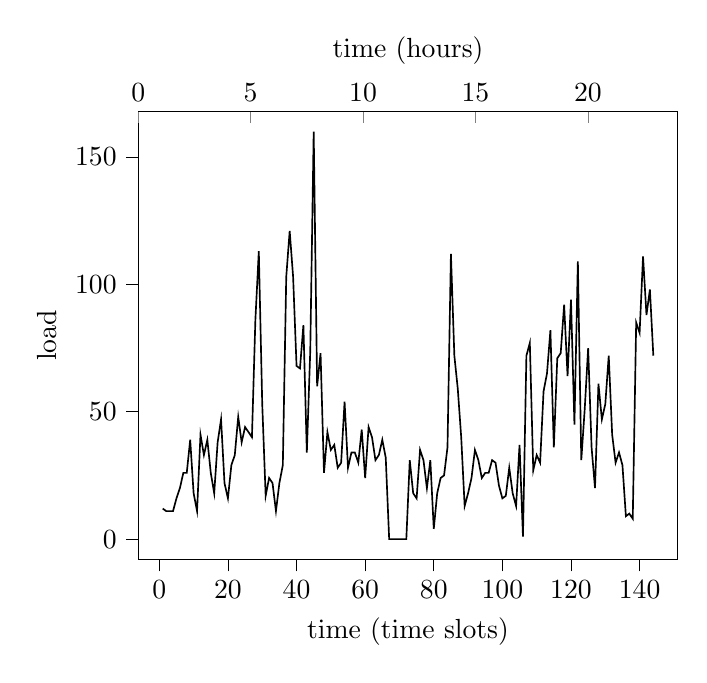
\begin{tikzpicture}

\begin{axis}[
tick align=outside,
tick pos=left,
x grid style={white!69.0196078431373!black},
xlabel={time (time slots)},
xmin=-6.15, xmax=151.15,
xtick style={color=black},
y grid style={white!69.0196078431373!black},
ylabel={load},
ymin=-8, ymax=168,
ytick style={color=black}
]
\addplot [semithick]
table {%
1 12
2 11
3 11
4 11
5 16
6 20
7 26
8 26
9 39
10 18
11 11
12 41
13 33
14 39
15 26
16 18
17 38
18 47
19 22
20 16
21 29
22 33
23 48
24 38
25 44
26 42
27 40
28 86
29 113
30 53
31 17
32 24
33 22
34 11
35 22
36 29
37 103
38 121
39 103
40 68
41 67
42 84
43 34
44 74
45 160
46 60
47 73
48 26
49 42
50 35
51 37
52 28
53 30
54 54
55 28
56 34
57 34
58 30
59 43
60 24
61 44
62 40
63 31
64 33
65 39
66 32
67 0
68 0
69 0
70 0
71 0
72 0
73 31
74 18
75 16
76 35
77 31
78 20
79 31
80 4
81 18
82 24
83 25
84 36
85 112
86 72
87 59
88 40
89 13
90 18
91 24
92 35
93 31
94 24
95 26
96 26
97 31
98 30
99 21
100 16
101 17
102 28
103 18
104 13
105 37
106 1
107 72
108 77
109 27
110 33
111 30
112 58
113 65
114 82
115 36
116 71
117 73
118 92
119 64
120 94
121 45
122 109
123 31
124 51
125 75
126 36
127 20
128 61
129 47
130 53
131 72
132 41
133 30
134 34
135 29
136 9
137 10
138 8
139 85
140 81
141 111
142 88
143 98
144 72
};
\end{axis}
\begin{axis}[
xmin=0,xmax=24,
axis y line=none,
axis x line*=top,
xlabel=time (hours)]
\addplot [draw=none,forget plot] {x};
\end{axis}

\end{tikzpicture}
}
    \caption{2009-0}
    \end{subfigure}
    \begin{subfigure}[b]{.32\linewidth}
    \resizebox{\textwidth}{!}{% This file was created by tikzplotlib v0.9.9.
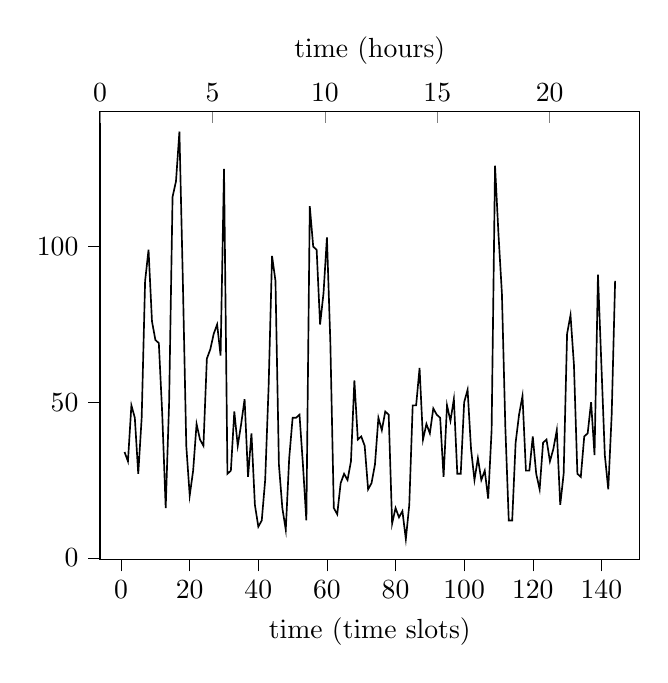
\begin{tikzpicture}

\begin{axis}[
tick align=outside,
tick pos=left,
x grid style={white!69.0196078431373!black},
xlabel={time (time slots)},
xmin=-6.15, xmax=151.15,
xtick style={color=black},
y grid style={white!69.0196078431373!black},
% ylabel={load},
ymin=-0.550000000000001, ymax=143.55,
ytick style={color=black}
]
\addplot [semithick]
table {%
1 34
2 31
3 49
4 45
5 27
6 45
7 89
8 99
9 76
10 70
11 69
12 46
13 16
14 50
15 116
16 121
17 137
18 89
19 36
20 20
21 28
22 43
23 38
24 36
25 64
26 67
27 72
28 75
29 65
30 125
31 27
32 28
33 47
34 36
35 43
36 51
37 26
38 40
39 17
40 10
41 12
42 25
43 55
44 97
45 89
46 30
47 16
48 9
49 32
50 45
51 45
52 46
53 30
54 12
55 113
56 100
57 99
58 75
59 85
60 103
61 69
62 16
63 14
64 24
65 27
66 25
67 31
68 57
69 38
70 39
71 36
72 22
73 24
74 30
75 45
76 41
77 47
78 46
79 11
80 16
81 13
82 15
83 6
84 17
85 49
86 49
87 61
88 38
89 43
90 40
91 48
92 46
93 45
94 26
95 49
96 44
97 51
98 27
99 27
100 50
101 54
102 35
103 25
104 32
105 25
106 28
107 19
108 41
109 126
110 104
111 85
112 42
113 12
114 12
115 37
116 46
117 52
118 28
119 28
120 39
121 27
122 22
123 37
124 38
125 31
126 35
127 41
128 17
129 27
130 72
131 78
132 62
133 27
134 26
135 39
136 40
137 50
138 33
139 91
140 62
141 33
142 22
143 46
144 89
};
\end{axis}
\begin{axis}[
xmin=0,xmax=24,
axis y line=none,
axis x line*=top,
xlabel=time (hours)]
\addplot [draw=none,forget plot] {x};
\end{axis}

\end{tikzpicture}
}
    \caption{2009-1}
    \end{subfigure}
    \begin{subfigure}[b]{.32\linewidth}
    \resizebox{\textwidth}{!}{% This file was created by tikzplotlib v0.9.9.
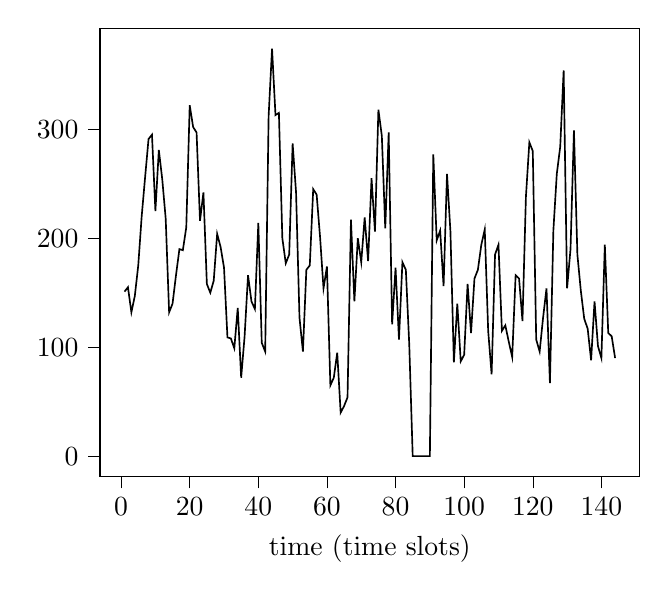
\begin{tikzpicture}

\begin{axis}[
tick align=outside,
tick pos=left,
x grid style={white!69.0196078431373!black},
xlabel={time (time slots)},
xmin=-6.15, xmax=151.15,
xtick style={color=black},
y grid style={white!69.0196078431373!black},
% ylabel={load},
ymin=-18.7, ymax=392.7,
ytick style={color=black}
]
\addplot [semithick]
table {%
1 151
2 155
3 132
4 147
5 175
6 220
7 256
8 291
9 295
10 225
11 281
12 254
13 218
14 132
15 140
16 166
17 190
18 189
19 210
20 322
21 302
22 297
23 216
24 242
25 158
26 150
27 161
28 204
29 192
30 173
31 109
32 108
33 99
34 136
35 72
36 110
37 166
38 142
39 135
40 214
41 104
42 96
43 312
44 374
45 313
46 315
47 200
48 177
49 185
50 287
51 242
52 127
53 96
54 171
55 175
56 245
57 240
58 201
59 154
60 174
61 65
62 72
63 95
64 40
65 46
66 54
67 217
68 142
69 200
70 178
71 219
72 179
73 255
74 206
75 318
76 294
77 209
78 297
79 121
80 173
81 107
82 178
83 171
84 102
85 0
86 0
87 0
88 0
89 0
90 0
91 277
92 198
93 207
94 156
95 259
96 206
97 86
98 140
99 87
100 93
101 158
102 113
103 163
104 171
105 194
106 208
107 115
108 75
109 185
110 194
111 115
112 120
113 105
114 91
115 166
116 163
117 124
118 238
119 288
120 280
121 107
122 96
123 127
124 154
125 67
126 207
127 259
128 284
129 354
130 154
131 190
132 299
133 185
134 152
135 126
136 117
137 88
138 142
139 101
140 90
141 194
142 113
143 110
144 90
};
\end{axis}

\end{tikzpicture}
}
    \caption{2010}
    \end{subfigure}
    \caption{Facebook MapReduce workloads.}
    \label{fig:facebook:histogram}
\end{figure}

\begin{figure}
    \begin{subfigure}[b]{.33\linewidth}
    \resizebox{\textwidth}{!}{% This file was created by tikzplotlib v0.9.9.
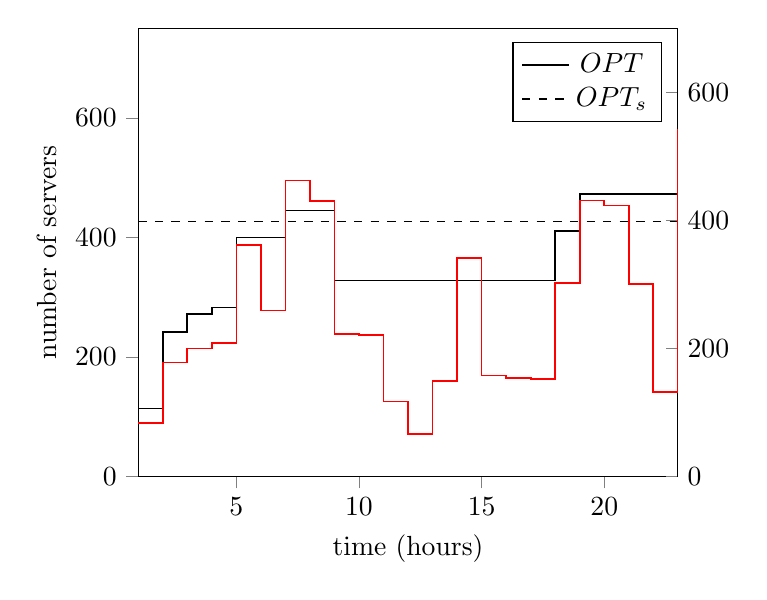
\begin{tikzpicture}

\begin{axis}[
legend pos=north east,
tick align=outside,
tick pos=left,
% x grid style={white!69.0196078431373!black},
xlabel={time (hours)},
xmin=1, xmax=23,
% xtick style={color=black},
% y grid style={white!69.0196078431373!black},
ylabel={number of servers},
ymin=0, ymax=750,
% ytick style={color=black}
]
\addplot [semithick, black, const plot mark left]
table {%
1 114
2 242
3 272
4 283
5 400
6 400
7 445
8 445
9 328
10 328
11 328
12 328
13 328
14 328
15 328
16 328
17 328
18 411
19 473
20 473
21 473
22 473
23 479
};
\addlegendentry{$OPT$}

\draw[dashed, color=black] (axis cs:\pgfkeysvalueof{/pgfplots/xmin},426) -- (axis cs:\pgfkeysvalueof{/pgfplots/xmax},426);
\addlegendimage{dashed, color=black}
\addlegendentry{$OPT_s$}
\end{axis}

\begin{axis}[
axis y line*=right,
axis x line=none,
xmin=1, xmax=23,
ymin=0, ymax=700,
% ylabel=load
]
\addplot [semithick, red, const plot mark left]
table {%
1 84
2 178
3 200
4 208
5 361
6 259
7 462
8 430
9 223
10 221
11 117
12 66
13 149
14 341
15 158
16 154
17 152
18 302
19 431
20 423
21 301
22 132
23 542
};
\end{axis}

\end{tikzpicture}
}
    \caption{2009-0}
    \end{subfigure}
    \begin{subfigure}[b]{.3075\linewidth}
    \resizebox{\textwidth}{!}{% This file was created by tikzplotlib v0.9.9.
\begin{tikzpicture}

\begin{axis}[
legend pos=north east,
axis y line*=right,
axis x line=none,
xmin=1, xmax=23,
ymin=0, ymax=750,
% ylabel=load
]
\addplot [semithick, red, const plot mark left, name path=A]
table {%
1 246
2 441
3 552
4 235
5 437
6 241
7 216
8 246
9 378
10 425
11 202
12 203
13 178
14 217
15 258
16 252
17 198
18 418
19 210
20 212
21 283
22 241
23 349
};
\addlegendentry{load}

\addplot+[draw=none,domain=0:24,name path=B] {-10000};
\addplot+[red!5] fill between[of=A and B];
\end{axis}

\begin{axis}[
legend pos=north west,
tick align=outside,
tick pos=left,
% x grid style={white!69.0196078431373!black},
xlabel={time (hours)},
xmin=1, xmax=23,
% xtick style={color=black},
% y grid style={white!69.0196078431373!black},
% ylabel={number of servers},
ymin=0, ymax=800,
% ytick style={color=black}
]
\addplot [semithick, black, const plot mark left]
table {%
1 334
2 506
3 506
4 484
5 484
6 422
7 422
8 422
9 422
10 422
11 328
12 328
13 328
14 328
15 328
16 328
17 328
18 370
19 352
20 352
21 352
22 352
23 352
};
\addlegendentry{$OPT$}

\draw[dashed, color=black] (axis cs:\pgfkeysvalueof{/pgfplots/xmin},424) -- (axis cs:\pgfkeysvalueof{/pgfplots/xmax},424);
\addlegendimage{dashed, color=black}
\addlegendentry{$OPT_s$}
\end{axis}

\end{tikzpicture}
}
    \caption{2009-1}
    \end{subfigure}
    \begin{subfigure}[b]{.3475\linewidth}
    \resizebox{\textwidth}{!}{% This file was created by tikzplotlib v0.9.9.
\begin{tikzpicture}

\begin{axis}[
legend pos=north east,
axis y line*=right,
axis x line=none,
xmin=1, xmax=23,
ymin=0, ymax=2500,
ylabel=load
]
\addplot [semithick, red, const plot mark left, name path=A]
table {%
1 1043
2 1646
3 1118
4 1564
5 1010
6 741
7 1259
8 1551
9 1096
10 911
11 687
12 1432
13 1223
14 380
15 818
16 903
17 1051
18 822
19 1089
20 892
21 1490
22 977
23 739
};
\addlegendentry{load}

\addplot+[draw=none,domain=0:24,name path=B] {-10000};
\addplot+[red!5] fill between[of=A and B];
\end{axis}

\begin{axis}[
legend pos=north west,
tick align=outside,
tick pos=left,
% x grid style={white!69.0196078431373!black},
xlabel={time (hours)},
xmin=1, xmax=23,
% xtick style={color=black},
% y grid style={white!69.0196078431373!black},
% ylabel={number of servers},
ymin=0, ymax=3000,
% ytick style={color=black}
]
\addplot [semithick, black, const plot mark left]
table {%
1 1000
2 1000
3 1000
4 1000
5 1000
6 1000
7 1000
8 1000
9 1000
10 1000
11 1000
12 1000
13 1000
14 1000
15 1000
16 1000
17 1000
18 1000
19 1000
20 1000
21 1000
22 1000
23 1000
};
\addlegendentry{$OPT$}

\draw[dashed, color=black] (axis cs:\pgfkeysvalueof{/pgfplots/xmin},1000) -- (axis cs:\pgfkeysvalueof{/pgfplots/xmax},1000);
\addlegendimage{dashed, color=black}
\addlegendentry{$OPT_s$}
\end{axis}

\end{tikzpicture}
}
    \caption{2010}
    \end{subfigure}
    \caption{Optimal dynamic and static offline schedules for the last day of the Facebook workloads. The left y axis shows the number of servers of the static and dynamic offline optima at a given time (black). The right y axis shows the number of jobs (i.e., the load) at a given time (red).}
    \label{fig:facebook:schedule}
\end{figure}

\begin{table}
    \centering
    \begin{tabularx}{\textwidth}{>{\bfseries}l|X|X|X}
        characteristic & 2009-0 & 2009-1 & 2010 \\\hline
        duration & 1 day & 1 day & 1 day \\
        number of jobs & 6 thousand & 7 thousand & 24 thousand \\
        median interarrival time & 7 seconds & 7 seconds & 2 seconds \\
        PMR & 3.91 & 2.97 & 2.2 \\
        TPMR & 2.04 & 1.93 & 1.69 \\
        mean peak distance & 95 minutes & 106 minutes & 87 minutes \\
        mean valley length & 44 minutes & 36 minutes & 35 minutes \\
        % diurnal pattern & \emph{trace too short} & \emph{trace too short} & \emph{trace too short} \\
    \caption{Characteristics of Facebook's MapReduce workloads.}
    \end{tabularx}
    \label{tab:facebook}
\end{table}

\paragraph{Los Alamos National Lab HPC Traces~\cite{Amvrosiadis2018_3, Amvrosiadis2018, Amvrosiadis2018_2}} This trace comprises two separate traces from high-performance computing clusters from Los Alamos National Lab (LANL). The traces were published by \citeauthor*{Amvrosiadis2018}~\cite{Amvrosiadis2018} as part of the Atlas project at Carnegie Mellon University.

The first trace is from the Mustang cluster, a general-purpose cluster consisting of 1600 homogeneous servers. Jobs were assigned to entire servers. The dataset covers 61 months from October 2011 to November 2016 and is shown in \cref{fig:los_alamos:histogram}. Note that the PMR is large at $622$ due to some outliers in the data. The median job duration is roughly 7 minutes, although the trace includes some extremely long-running outliers, resulting in a mean job duration of over 2.5 hours. In the trace, jobs were assigned to one or multiple servers. To normalize the trace, we consider each job once for each server it was processed on. \Cref{fig:los_alamos:schedule} shows the dynamic and static offline optimal schedules under our second model.

The second trace is from the Trinity supercomputer. This trace is very similar to the Mustang trace but includes an even more significant number of long-running jobs. We, therefore, do not consider this trace in our analysis.

\paragraph{Microsoft Fiddle Trace~\cite{Jeon2019}} This trace consists of deep neural network training workloads on internal servers from Microsoft. The trace was published as part of the Fiddle project from Microsoft Research. The jobs are run on a heterogeneous set of servers which we group based on the number of GPUs of each server. There are 321 servers with two GPUs and 231 servers with eight GPUs. The median job duration is just below 15 minutes. The load profiles are visualized in \cref{fig:microsoft:histogram}.

The CPU utilization of the trace is extremely low, with more than 80\% of servers running with utilization 30\% or less~\cite{Santhanam2019}. However, memory utilization is high, with an average of more than 80\% indicating that overall server utilization is already very high~\cite{Santhanam2019}. Again, the PMR is rather large at 89.43 due to outliers.

In our model, we adjust the runtime of jobs relative to the number of available GPUs in the respective server, i.e., the average runtime of jobs on a 2-GPU-server is four times as long as the average runtime of jobs on an 8-GPU-server. We adjust for the increased energy consumption of a server with eight GPUs by increasing the energy consumption of servers with two GPUs by a factor of 4.2. We also associate a fifteen times higher switching cost with servers with eight GPUs.

The dynamic and static offline optimal schedules under our second model are shown in \cref{fig:microsoft:schedule}. Note that under the given load servers with two GPUs are preferred to servers with eight GPUs when they are only needed for a short period due to their lower switching costs. This might seem counterintuitive at first, as 2-GPU-servers seem to be strictly better than 8-GPU-servers as the operating and switching cost of 8-GPU-servers is worse by a factor greater than four than the respective cost of 2-GPU-servers. However, we assume an average job runtime of 7.5 minutes on 8-GPU-servers as opposed to an average job runtime of 30 minutes on 2-GPU-servers (a factor of four), implying that 8-GPU-servers can process more than four jobs in an hour without a significant increase in delay, whereas 2-GPU-servers are limited to one job per time slot.

\paragraph{Alibaba Trace~\cite{Alibaba2018}} This trace consists of a mixture of long-running applications and batch jobs. We are using their trace from 2018, covering eight days. The trace is visualized in \cref{fig:alibaba:histogram}, the dynamic and static offline optimal schedules under our second model are shown in \cref{fig:alibaba:schedule}. The jobs are processed on 4000 homogeneous servers. In our models, we assume a total of 10,000 servers to ensure that the number of servers is not a bottleneck. Jobs themselves are grouped into 11 types which we further simplify to 4 types based on their average runtime. We consider \emph{short}, \emph{medium}, \emph{long}, and \emph{very long} jobs. Their average runtime in the trace is shown in \cref{tab:alibaba:job_types}. The mean job duration is just below 15 minutes. The median job duration is 8 seconds, and the mean job duration is just over 1.5 minutes.

\begin{table}
    \centering
    \begin{tabularx}{\textwidth}{>{\bfseries}l|c}
        job type & mean runtime \\\hline
        short & 68 seconds \\
        medium & 196 seconds \\
        long & 534 seconds \\
        very long & 1180 seconds \\
    \caption{Characterization of the job types of the Alibaba trace.}
    \end{tabularx}
    \label{tab:alibaba:job_types}
\end{table}

Data from a previous trace indicates that mean CPU utilization varies between 10\% and 40\% while mean memory utilization varies between 40\% and 65\%~\cite{Lu2017}. This indicates that the overall server utilization is not optimal.

In our model, we scale job runtimes by a factor of 2.5 from short to very long jobs, roughly matching the runtimes of jobs from the trace.

\begin{figure}
    \begin{subfigure}[b]{.3425\linewidth}
    \resizebox{\textwidth}{!}{% This file was created by tikzplotlib v0.9.9.
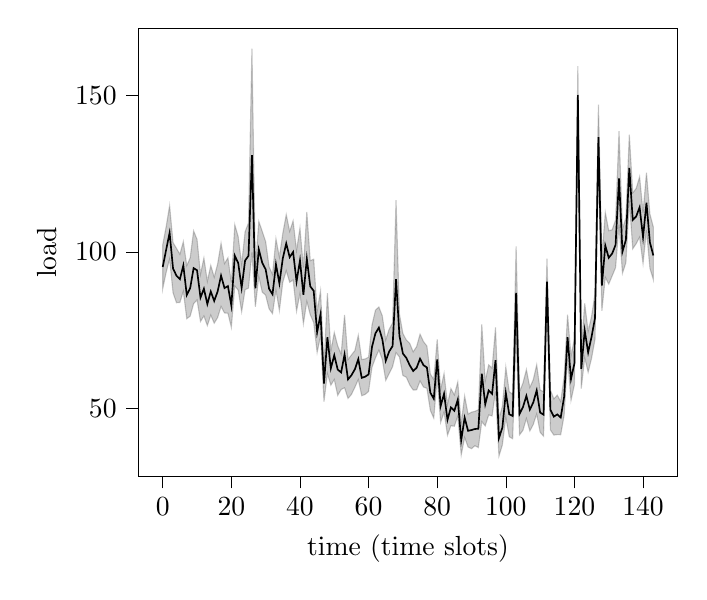
\begin{tikzpicture}

\begin{axis}[
tick align=outside,
tick pos=left,
x grid style={white!69.0196078431373!black},
xlabel={time (time slots)},
xmin=-7.15, xmax=150.15,
xtick style={color=black},
y grid style={white!69.0196078431373!black},
ylabel={load},
ymin=28.2849782490484, ymax=171.400720500272,
ytick style={color=black}
]
\path [draw=black, fill=black, opacity=0.2]
(axis cs:0,102.293909733551)
--(axis cs:0,88.2570690592713)
--(axis cs:1,93.4765497553018)
--(axis cs:2,97.7530587275693)
--(axis cs:3,86.9439233278956)
--(axis cs:4,83.7712751495378)
--(axis cs:5,83.8595704187058)
--(axis cs:6,87.4492930940729)
--(axis cs:7,78.6575584556824)
--(axis cs:8,79.5031266992931)
--(axis cs:9,83.4768896139206)
--(axis cs:10,84.6759787928222)
--(axis cs:11,77.7783442088091)
--(axis cs:12,79.5494834148994)
--(axis cs:13,76.4580614464383)
--(axis cs:14,79.8323137574769)
--(axis cs:15,77.238240891789)
--(axis cs:16,79.0176046764546)
--(axis cs:17,82.5918977705275)
--(axis cs:18,80.5129825992387)
--(axis cs:19,80.4093257205003)
--(axis cs:20,75.8719412724307)
--(axis cs:21,89.1316612289288)
--(axis cs:22,87.7784801522567)
--(axis cs:23,80.8613376835237)
--(axis cs:24,87.9407286568787)
--(axis cs:25,88.4441952147907)
--(axis cs:26,99.8377514953779)
--(axis cs:27,82.4729472539424)
--(axis cs:28,92.1181348559)
--(axis cs:29,87.1662588363241)
--(axis cs:30,86.1648994018488)
--(axis cs:31,81.8153208265362)
--(axis cs:32,80.2848015225666)
--(axis cs:33,87.7914627514954)
--(axis cs:34,81.2480288200109)
--(axis cs:35,90.3231375747689)
--(axis cs:36,94.0078167482327)
--(axis cs:37,90.301318651441)
--(axis cs:38,91.0621941272431)
--(axis cs:39,81.0538336052202)
--(axis cs:40,86.7768488308864)
--(axis cs:41,77.0454051114736)
--(axis cs:42,84.2014002175095)
--(axis cs:43,79.943243610658)
--(axis cs:44,77.4161228928766)
--(axis cs:45,67.8759516041327)
--(axis cs:46,73.1824361065797)
--(axis cs:47,52.213023382273)
--(axis cs:48,61.1465470364328)
--(axis cs:49,57.443515497553)
--(axis cs:50,59.2738580750408)
--(axis cs:51,54.2004486133768)
--(axis cs:52,56.0547852093529)
--(axis cs:53,56.6154159869494)
--(axis cs:54,53.2134991843393)
--(axis cs:55,54.4917754214247)
--(axis cs:56,56.7627786840674)
--(axis cs:57,59.2508156606852)
--(axis cs:58,54.09230560087)
--(axis cs:59,54.4956498096792)
--(axis cs:60,55.4433795541055)
--(axis cs:61,63.2101005981512)
--(axis cs:62,66.1526644915715)
--(axis cs:63,68.6571506253399)
--(axis cs:64,65.653955954323)
--(axis cs:65,58.9832789559543)
--(axis cs:66,61.1518488308864)
--(axis cs:67,63.384448069603)
--(axis cs:68,67.8308863512779)
--(axis cs:69,66.4802882001088)
--(axis cs:70,60.5184203371398)
--(axis cs:71,59.9963974986406)
--(axis cs:72,57.5238580750408)
--(axis cs:73,55.9103452963567)
--(axis cs:74,55.9381457313757)
--(axis cs:75,58.8077759651985)
--(axis cs:76,56.8678629690049)
--(axis cs:77,56.4520799347471)
--(axis cs:78,49.4161228928766)
--(axis cs:79,46.9261827079935)
--(axis cs:80,59.7202963567156)
--(axis cs:81,45.5475122349103)
--(axis cs:82,48.8830886351278)
--(axis cs:83,41.4662180532898)
--(axis cs:84,44.4964654703643)
--(axis cs:85,44.3459081022295)
--(axis cs:86,47.5729336595976)
--(axis cs:87,35.130165851006)
--(axis cs:88,40.7707313757477)
--(axis cs:89,37.7206362153344)
--(axis cs:90,37.1803969548668)
--(axis cs:91,38.1146003262643)
--(axis cs:92,37.5334420880914)
--(axis cs:93,45.8475394235998)
--(axis cs:94,44.4517400761283)
--(axis cs:95,47.9382816748233)
--(axis cs:96,47.6332245785753)
--(axis cs:97,55.4692088091354)
--(axis cs:98,34.7902392604676)
--(axis cs:99,38.3958673191952)
--(axis cs:100,47.2095568243611)
--(axis cs:101,41.001155519304)
--(axis cs:102,40.3446846112017)
--(axis cs:103,73.1284665579119)
--(axis cs:104,41.5866639477977)
--(axis cs:105,43.04588091354)
--(axis cs:106,46.820826536161)
--(axis cs:107,42.8232735182164)
--(axis cs:108,44.8975666122893)
--(axis cs:109,48.2442903752039)
--(axis cs:110,42.4265905383361)
--(axis cs:111,41.1706769983687)
--(axis cs:112,82.2564573137575)
--(axis cs:113,43.1617247007617)
--(axis cs:114,41.5231229597388)
--(axis cs:115,41.6744423286181)
--(axis cs:116,41.6337731229597)
--(axis cs:117,47.8305903155604)
--(axis cs:118,66.0195865070729)
--(axis cs:119,52.5657644178455)
--(axis cs:120,57.6513873775843)
--(axis cs:121,140.992519042437)
--(axis cs:122,56.3764961915125)
--(axis cs:123,66.2161316648531)
--(axis cs:124,61.5605277475517)
--(axis cs:125,66.0799782372144)
--(axis cs:126,72.1264961915125)
--(axis cs:127,127.082018498368)
--(axis cs:128,81.149415125136)
--(axis cs:129,91.9145130576714)
--(axis cs:130,89.7028019586507)
--(axis cs:131,92.3431719260065)
--(axis cs:132,94.978577257889)
--(axis cs:133,108.670361806311)
--(axis cs:134,93.1548558215452)
--(axis cs:135,96.5391050054407)
--(axis cs:136,116.370851468988)
--(axis cs:137,100.963547334059)
--(axis cs:138,102.624455930359)
--(axis cs:139,104.709874863983)
--(axis cs:140,96.2629216539717)
--(axis cs:141,106.955794341676)
--(axis cs:142,94.7566648531012)
--(axis cs:143,91.1413220892274)
--(axis cs:143,107.934507616975)
--(axis cs:143,107.934507616975)
--(axis cs:142,112.125068008705)
--(axis cs:141,125.269246463547)
--(axis cs:140,112.56569640914)
--(axis cs:139,124.015573993471)
--(axis cs:138,120.251564200218)
--(axis cs:137,118.841811751904)
--(axis cs:136,137.44348476605)
--(axis cs:135,110.929066920566)
--(axis cs:134,107.208446681175)
--(axis cs:133,138.575149619151)
--(axis cs:132,110.207358541893)
--(axis cs:131,107.060935799782)
--(axis cs:130,106.760201305767)
--(axis cs:129,112.633569096844)
--(axis cs:128,97.8228373231774)
--(axis cs:127,147.02380304679)
--(axis cs:126,86.6896762785637)
--(axis cs:125,79.4353917301415)
--(axis cs:124,74.6337051142546)
--(axis cs:123,83.5605277475517)
--(axis cs:122,68.9980957562568)
--(axis cs:121,159.283324265506)
--(axis cs:120,72.300598476605)
--(axis cs:119,66.751768226333)
--(axis cs:118,79.9591947769314)
--(axis cs:117,60.1431583242655)
--(axis cs:116,52.2323857453754)
--(axis cs:115,54.2736670293798)
--(axis cs:114,53.0549510337323)
--(axis cs:113,55.9255304678999)
--(axis cs:112,97.8251767264818)
--(axis cs:111,55.3794861337684)
--(axis cs:110,55.8929445350734)
--(axis cs:109,63.9782490483959)
--(axis cs:108,59.1849510603589)
--(axis cs:107,56.7059543230016)
--(axis cs:106,62.4491571506253)
--(axis cs:105,58.1299619358347)
--(axis cs:104,55.3601141924959)
--(axis cs:103,101.76101141925)
--(axis cs:102,54.5269168026101)
--(axis cs:101,55.3924687330071)
--(axis cs:100,63.2522430668842)
--(axis cs:99,50.761759108211)
--(axis cs:98,46.6941952147906)
--(axis cs:97,75.9178221859706)
--(axis cs:96,62.8654159869494)
--(axis cs:95,63.9365144100054)
--(axis cs:94,58.7691000543774)
--(axis cs:93,76.838023382273)
--(axis cs:92,49.6122213159326)
--(axis cs:91,49.1128330614464)
--(axis cs:90,48.8268080478521)
--(axis cs:89,48.2183931484502)
--(axis cs:88,54.0093800978793)
--(axis cs:87,45.2105084284937)
--(axis cs:86,58.4961256117455)
--(axis cs:85,54.3427814029364)
--(axis cs:84,56.3588907014682)
--(axis cs:83,51.3167482327352)
--(axis cs:82,61.1913404023926)
--(axis cs:81,56.0580478520935)
--(axis cs:80,72.0507069059271)
--(axis cs:79,59.2642060902664)
--(axis cs:78,61.0149537792278)
--(axis cs:77,69.9520119630234)
--(axis cs:76,71.3806416530723)
--(axis cs:75,73.7303561718325)
--(axis cs:74,69.7633904295813)
--(axis cs:73,68.0936650353453)
--(axis cs:72,70.7802474170745)
--(axis cs:71,71.8613376835237)
--(axis cs:70,73.9522158781947)
--(axis cs:69,80.1324768896139)
--(axis cs:68,116.484026644916)
--(axis cs:67,77.2654295812942)
--(axis cs:66,75.3376835236542)
--(axis cs:65,71.9083741163676)
--(axis cs:64,79.5914899401849)
--(axis cs:63,82.4129282218597)
--(axis cs:62,81.3950516585101)
--(axis cs:61,76.6725802066341)
--(axis cs:60,66.385331702012)
--(axis cs:59,65.8283713974986)
--(axis cs:58,65.6219412724307)
--(axis cs:57,73.3854676454595)
--(axis cs:56,68.4687330070691)
--(axis cs:55,67.1064437194127)
--(axis cs:54,65.6239124524198)
--(axis cs:53,79.8786704730832)
--(axis cs:52,67.3333333333333)
--(axis cs:51,70.0311310494834)
--(axis cs:50,74.2591082109842)
--(axis cs:49,68.365823817292)
--(axis cs:48,86.804173463839)
--(axis cs:47,63.4638390429581)
--(axis cs:46,87.6275149537792)
--(axis cs:45,80.9894643828167)
--(axis cs:44,97.6704051114736)
--(axis cs:43,97.2047988036977)
--(axis cs:42,112.724782490484)
--(axis cs:41,95.0084964654704)
--(axis cs:40,107.655043501903)
--(axis cs:39,100.453779227841)
--(axis cs:38,109.899061990212)
--(axis cs:37,106.553697661773)
--(axis cs:36,111.909393692224)
--(axis cs:35,105.955886351278)
--(axis cs:34,98.3259923871669)
--(axis cs:33,104.199157150625)
--(axis cs:32,92.7971723762915)
--(axis cs:31,95.2658374116368)
--(axis cs:30,103.306348558999)
--(axis cs:29,106.604472539424)
--(axis cs:28,109.735114192496)
--(axis cs:27,94.8692224034802)
--(axis cs:26,164.895459488853)
--(axis cs:25,109.250679717238)
--(axis cs:24,106.438689505166)
--(axis cs:23,96.0057775965198)
--(axis cs:22,104.830682436107)
--(axis cs:21,108.680261011419)
--(axis cs:20,90.1990212071778)
--(axis cs:19,98.1153480152257)
--(axis cs:18,96.2733822729744)
--(axis cs:17,102.77222675367)
--(axis cs:16,96.1714926590538)
--(axis cs:15,91.9235318107667)
--(axis cs:14,95.6881457313758)
--(axis cs:13,90.5901984774334)
--(axis cs:12,98.0657966286025)
--(axis cs:11,92.864396411093)
--(axis cs:10,104.000203915171)
--(axis cs:9,106.704526916803)
--(axis cs:8,98.1082109842306)
--(axis cs:7,95.6343800978793)
--(axis cs:6,103.292890157694)
--(axis cs:5,99.2375611745514)
--(axis cs:4,101.132205002719)
--(axis cs:3,102.973558999456)
--(axis cs:2,114.800774877651)
--(axis cs:1,108.076672104405)
--(axis cs:0,102.293909733551)
--cycle;

\addplot [semithick]
table {%
0 95.1799891245242
1 100.728113104948
2 106.075040783034
3 94.7134312126155
4 92.405111473627
5 91.2822185970636
6 95.6601413811854
7 86.2691680261011
8 88.457857531267
9 94.815660685155
10 94.1305057096248
11 85.4067427949973
12 88.2468733007069
13 83.3518216421969
14 87.3572593800979
15 84.342033713975
16 87.3670473083197
17 92.4138118542686
18 88.4567699836868
19 89.0734094616639
20 82.8711256117455
21 98.7857531266993
22 96.4333877107123
23 88.5252854812398
24 97.2289287656335
25 98.7547580206634
26 130.852093529092
27 88.3621533442088
28 100.802066340402
29 96.5296356715606
30 94.4072865687874
31 88.215878194671
32 86.4616639477977
33 96.0222947253942
34 89.9690048939641
35 97.9603045133225
36 102.696030451332
37 98.3186514410005
38 99.963023382273
39 90.5301794453507
40 97.2452419793366
41 86.3056008700381
42 97.821098423056
43 88.9978249048396
44 87.5617183251767
45 74.3284393692224
46 80.0940728656879
47 57.9543230016313
48 72.7340946166395
49 62.8363240891789
50 66.994562262099
51 62.4339314845024
52 61.5198477433388
53 67.2680804785209
54 59.310494834149
55 60.6247960848287
56 62.5252854812398
57 65.7857531266993
58 59.7971723762915
59 60.1636759108211
60 60.889613920609
61 69.7014681892333
62 73.9978249048396
63 75.8227297444263
64 72.1337683523654
65 65.2300163132137
66 68.1990212071778
67 69.9483414899402
68 91.2729744426319
69 73.1718325176727
70 67.5622620989668
71 66.1489940184883
72 63.8069603045133
73 61.9766177270256
74 62.9961935834693
75 65.9037520391517
76 63.8390429581294
77 63.1060358890701
78 55.0696030451332
79 53.1256117455139
80 65.6487221315933
81 50.7890157694399
82 54.7025557368135
83 46.4029363784666
84 50.3708537248505
85 49.2996193583469
86 52.8129418162045
87 39.8934203371398
88 47.0734094616639
89 42.8852637302882
90 43.1179989124524
91 43.4660141381185
92 43.557911908646
93 61.1386623164763
94 51.363240891789
95 55.7514953779228
96 54.6726481783578
97 65.4540511147363
98 40.552474170745
99 43.9140837411637
100 55.0217509516041
101 48.1772702555737
102 47.6014138118543
103 86.8928765633496
104 48.278955954323
105 50.4638390429581
106 54.0353452963567
107 49.6552474170745
108 51.9140837411637
109 55.7868406742795
110 48.7199564980968
111 48.0413268080478
112 90.5301794453507
113 49.5778019586507
114 47.4162132752992
115 48.1158868335147
116 47.1316648531012
117 53.7350380848749
118 72.8084874863983
119 59.4020674646355
120 64.4162132752992
121 150.01795429815
122 62.639281828074
123 74.936887921654
124 67.9167573449402
125 72.9221980413493
126 78.8911860718172
127 136.638737758433
128 89.2655059847661
129 102.01795429815
130 98.1126224156692
131 99.4760609357998
132 102.248639825898
133 123.4640914037
134 100.075625680087
135 103.822089227421
136 126.836235038085
137 110.215995647443
138 111.311751904244
139 114.233405875952
140 104.688248095756
141 115.67845484222
142 103.048422198041
143 98.8579978237214
};
\end{axis}

\end{tikzpicture}
}
    \caption{LANL Mustang}\label{fig:los_alamos:histogram}
    \end{subfigure}
    \begin{subfigure}[b]{.32\linewidth}
    \resizebox{\textwidth}{!}{% This file was created by tikzplotlib v0.9.9.
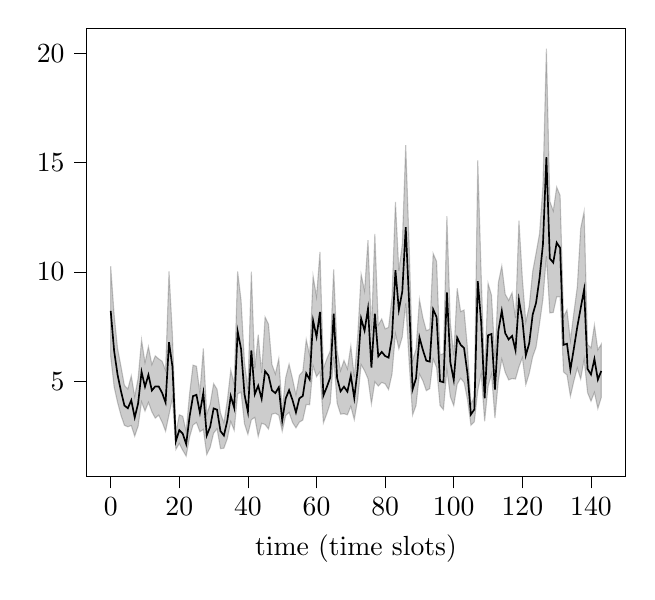
\begin{tikzpicture}

\begin{axis}[
tick align=outside,
tick pos=left,
x grid style={white!69.0196078431373!black},
xlabel={time (time slots)},
xmin=-7.15, xmax=150.15,
xtick style={color=black},
y grid style={white!69.0196078431373!black},
% ylabel={load},
ymin=0.652554744525547, ymax=21.1430656934307,
ytick style={color=black}
]
\path [draw=black, fill=black, opacity=0.2]
(axis cs:0,10.2636861313869)
--(axis cs:0,6.14507299270073)
--(axis cs:1,4.75091240875912)
--(axis cs:2,4.04379562043796)
--(axis cs:3,3.45255474452555)
--(axis cs:4,2.99270072992701)
--(axis cs:5,2.92700729927007)
--(axis cs:6,2.98540145985401)
--(axis cs:7,2.4963503649635)
--(axis cs:8,2.95620437956204)
--(axis cs:9,4.06386861313869)
--(axis cs:10,3.64142335766423)
--(axis cs:11,4.04379562043796)
--(axis cs:12,3.61222627737226)
--(axis cs:13,3.32116788321168)
--(axis cs:14,3.45894160583942)
--(axis cs:15,3.13868613138686)
--(axis cs:16,2.72171532846715)
--(axis cs:17,3.47992700729927)
--(axis cs:18,4.2463503649635)
--(axis cs:19,1.89051094890511)
--(axis cs:20,2.16697080291971)
--(axis cs:21,1.85401459854015)
--(axis cs:22,1.58394160583942)
--(axis cs:23,2.45255474452555)
--(axis cs:24,3.00729927007299)
--(axis cs:25,3.12317518248175)
--(axis cs:26,2.69799270072993)
--(axis cs:27,2.81021897810219)
--(axis cs:28,1.65693430656934)
--(axis cs:29,1.98540145985401)
--(axis cs:30,2.63412408759124)
--(axis cs:31,2.83941605839416)
--(axis cs:32,1.92609489051095)
--(axis cs:33,1.94890510948905)
--(axis cs:34,2.38686131386861)
--(axis cs:35,3.16788321167883)
--(axis cs:36,2.76642335766423)
--(axis cs:37,4.42974452554745)
--(axis cs:38,4.50912408759124)
--(axis cs:39,3.05656934306569)
--(axis cs:40,2.58394160583942)
--(axis cs:41,3.24726277372263)
--(axis cs:42,3.35766423357664)
--(axis cs:43,2.48175182481752)
--(axis cs:44,3.08667883211679)
--(axis cs:45,3.02919708029197)
--(axis cs:46,2.82390510948905)
--(axis cs:47,3.50182481751825)
--(axis cs:48,3.5456204379562)
--(axis cs:49,3.45255474452555)
--(axis cs:50,2.72262773722628)
--(axis cs:51,3.43065693430657)
--(axis cs:52,3.58394160583942)
--(axis cs:53,3.12408759124088)
--(axis cs:54,2.87591240875912)
--(axis cs:55,3.13868613138686)
--(axis cs:56,3.23266423357664)
--(axis cs:57,3.94799270072993)
--(axis cs:58,3.93339416058394)
--(axis cs:59,5.71441605839416)
--(axis cs:60,5.21715328467153)
--(axis cs:61,5.44343065693431)
--(axis cs:62,3.10127737226277)
--(axis cs:63,3.52554744525547)
--(axis cs:64,4.00638686131387)
--(axis cs:65,6.12317518248175)
--(axis cs:66,4.00638686131387)
--(axis cs:67,3.50273722627737)
--(axis cs:68,3.52463503649635)
--(axis cs:69,3.47445255474453)
--(axis cs:70,3.86770072992701)
--(axis cs:71,3.24726277372263)
--(axis cs:72,4.17518248175182)
--(axis cs:73,5.76642335766423)
--(axis cs:74,5.48813868613139)
--(axis cs:75,5.12408759124088)
--(axis cs:76,3.96989051094891)
--(axis cs:77,4.98266423357664)
--(axis cs:78,4.78740875912409)
--(axis cs:79,4.95620437956204)
--(axis cs:80,4.89051094890511)
--(axis cs:81,4.62682481751825)
--(axis cs:82,5.33394160583942)
--(axis cs:83,7.17518248175182)
--(axis cs:84,6.48813868613139)
--(axis cs:85,7.03558394160584)
--(axis cs:86,8.56843065693431)
--(axis cs:87,5.86131386861314)
--(axis cs:88,3.46624087591241)
--(axis cs:89,3.8978102189781)
--(axis cs:90,5.33576642335766)
--(axis cs:91,5.02828467153285)
--(axis cs:92,4.57664233576642)
--(axis cs:93,4.67153284671533)
--(axis cs:94,6.02919708029197)
--(axis cs:95,5.63412408759124)
--(axis cs:96,3.89689781021898)
--(axis cs:97,3.70711678832117)
--(axis cs:98,5.54653284671533)
--(axis cs:99,4.29835766423358)
--(axis cs:100,3.88959854014599)
--(axis cs:101,4.875)
--(axis cs:102,5.14416058394161)
--(axis cs:103,4.95529197080292)
--(axis cs:104,4.16788321167883)
--(axis cs:105,3)
--(axis cs:106,3.15328467153285)
--(axis cs:107,4.58302919708029)
--(axis cs:108,5.36405109489051)
--(axis cs:109,3.1742700729927)
--(axis cs:110,4.76642335766423)
--(axis cs:111,5.33576642335766)
--(axis cs:112,3.32025547445255)
--(axis cs:113,5.03375912408759)
--(axis cs:114,6.01459854014599)
--(axis cs:115,5.41605839416058)
--(axis cs:116,5.06843065693431)
--(axis cs:117,5.13047445255474)
--(axis cs:118,5.10857664233577)
--(axis cs:119,5.66423357664234)
--(axis cs:120,6.08759124087591)
--(axis cs:121,4.84671532846715)
--(axis cs:122,5.36496350364964)
--(axis cs:123,6.12317518248175)
--(axis cs:124,6.56843065693431)
--(axis cs:125,7.62773722627737)
--(axis cs:126,8.77098540145986)
--(axis cs:127,10.720802919708)
--(axis cs:128,8.12956204379562)
--(axis cs:129,8.15237226277372)
--(axis cs:130,8.86040145985401)
--(axis cs:131,8.86770072992701)
--(axis cs:132,5.43065693430657)
--(axis cs:133,5.29835766423358)
--(axis cs:134,4.32116788321168)
--(axis cs:135,5.00638686131387)
--(axis cs:136,5.61040145985401)
--(axis cs:137,5.1021897810219)
--(axis cs:138,6.00643382352941)
--(axis cs:139,4.49172794117647)
--(axis cs:140,4.09466911764706)
--(axis cs:141,4.49908088235294)
--(axis cs:142,3.75735294117647)
--(axis cs:143,4.26470588235294)
--(axis cs:143,6.70588235294118)
--(axis cs:143,6.70588235294118)
--(axis cs:142,6.44117647058824)
--(axis cs:141,7.58088235294118)
--(axis cs:140,6.52941176470588)
--(axis cs:139,6.69117647058824)
--(axis cs:138,12.7693014705882)
--(axis cs:137,11.9936131386861)
--(axis cs:136,9.31751824817518)
--(axis cs:135,8.12773722627737)
--(axis cs:134,6.87682481751825)
--(axis cs:133,8.27189781021898)
--(axis cs:132,7.94160583941606)
--(axis cs:131,13.4990875912409)
--(axis cs:130,13.8841240875912)
--(axis cs:129,12.7956204379562)
--(axis cs:128,13.2335766423358)
--(axis cs:127,20.2116788321168)
--(axis cs:126,13.9644160583942)
--(axis cs:125,11.7527372262774)
--(axis cs:124,10.8695255474453)
--(axis cs:123,10.0237226277372)
--(axis cs:122,8.43886861313869)
--(axis cs:121,7.72262773722628)
--(axis cs:120,9.70164233576642)
--(axis cs:119,12.3448905109489)
--(axis cs:118,7.8978102189781)
--(axis cs:117,9.05474452554745)
--(axis cs:116,8.70346715328467)
--(axis cs:115,8.98722627737226)
--(axis cs:114,10.2773722627737)
--(axis cs:113,9.51824817518248)
--(axis cs:112,6.05839416058394)
--(axis cs:111,8.94160583941606)
--(axis cs:110,9.48266423357664)
--(axis cs:109,5.21350364963504)
--(axis cs:108,9.84762773722628)
--(axis cs:107,15.1021897810219)
--(axis cs:106,4.31386861313869)
--(axis cs:105,3.94251824817518)
--(axis cs:104,6.52828467153285)
--(axis cs:103,8.26368613138686)
--(axis cs:102,8.18978102189781)
--(axis cs:101,9.25547445255475)
--(axis cs:100,6.18978102189781)
--(axis cs:99,7.68795620437956)
--(axis cs:98,12.5538321167883)
--(axis cs:97,6.27098540145985)
--(axis cs:96,6.21167883211679)
--(axis cs:95,10.4817518248175)
--(axis cs:94,10.8467153284672)
--(axis cs:93,7.38047445255474)
--(axis cs:92,7.32299270072993)
--(axis cs:91,7.91332116788321)
--(axis cs:90,8.74452554744525)
--(axis cs:89,6.47445255474453)
--(axis cs:88,5.94981751824818)
--(axis cs:87,11.1897810218978)
--(axis cs:86,15.8038321167883)
--(axis cs:85,11.271897810219)
--(axis cs:84,10.0565693430657)
--(axis cs:83,13.2080291970803)
--(axis cs:82,8.86222627737226)
--(axis cs:81,7.46715328467153)
--(axis cs:80,7.40237226277372)
--(axis cs:79,7.85401459854015)
--(axis cs:78,7.57755474452555)
--(axis cs:77,11.7390510948905)
--(axis cs:76,7.32116788321168)
--(axis cs:75,11.4543795620438)
--(axis cs:74,9.14416058394161)
--(axis cs:73,9.89963503649635)
--(axis cs:72,7.06021897810219)
--(axis cs:71,5.2043795620438)
--(axis cs:70,6.62043795620438)
--(axis cs:69,5.57664233576642)
--(axis cs:68,5.96350364963504)
--(axis cs:67,5.49178832116788)
--(axis cs:66,6.42335766423358)
--(axis cs:65,10.1240875912409)
--(axis cs:64,6.4014598540146)
--(axis cs:63,6.02919708029197)
--(axis cs:62,5.59215328467153)
--(axis cs:61,10.9178832116788)
--(axis cs:60,8.87591240875912)
--(axis cs:59,9.81843065693431)
--(axis cs:58,6.19069343065693)
--(axis cs:57,6.91332116788321)
--(axis cs:56,5.45985401459854)
--(axis cs:55,5.27919708029197)
--(axis cs:54,4.38686131386861)
--(axis cs:53,5.12408759124088)
--(axis cs:52,5.79014598540146)
--(axis cs:51,5.16879562043796)
--(axis cs:50,3.68613138686131)
--(axis cs:49,6.04470802919708)
--(axis cs:48,5.3448905109489)
--(axis cs:47,5.77463503649635)
--(axis cs:46,7.61405109489051)
--(axis cs:45,7.94434306569343)
--(axis cs:44,5.38686131386861)
--(axis cs:43,7.13229927007299)
--(axis cs:42,5.59306569343066)
--(axis cs:41,10.014598540146)
--(axis cs:40,4.63503649635036)
--(axis cs:39,5.87682481751825)
--(axis cs:38,8.71624087591241)
--(axis cs:37,10.0310218978102)
--(axis cs:36,4.86861313868613)
--(axis cs:35,5.52007299270073)
--(axis cs:34,4.13868613138686)
--(axis cs:33,3.1021897810219)
--(axis cs:32,3.56934306569343)
--(axis cs:31,4.64233576642336)
--(axis cs:30,4.89963503649635)
--(axis cs:29,3.96441605839416)
--(axis cs:28,3.48905109489051)
--(axis cs:27,6.5036496350365)
--(axis cs:26,4.48266423357664)
--(axis cs:25,5.69434306569343)
--(axis cs:24,5.74452554744526)
--(axis cs:23,4.4543795620438)
--(axis cs:22,2.71532846715328)
--(axis cs:21,3.40967153284672)
--(axis cs:20,3.47445255474453)
--(axis cs:19,2.64963503649635)
--(axis cs:18,7.11040145985401)
--(axis cs:17,10.0255474452555)
--(axis cs:16,5.50456204379562)
--(axis cs:15,5.9206204379562)
--(axis cs:14,6.0301094890511)
--(axis cs:13,6.16788321167883)
--(axis cs:12,5.76733576642336)
--(axis cs:11,6.59124087591241)
--(axis cs:10,5.86131386861314)
--(axis cs:9,6.9051094890511)
--(axis cs:8,5.15419708029197)
--(axis cs:7,4.30748175182482)
--(axis cs:6,5.25638686131387)
--(axis cs:5,4.6514598540146)
--(axis cs:4,4.81843065693431)
--(axis cs:3,5.68613138686131)
--(axis cs:2,6.51094890510949)
--(axis cs:1,8.05930656934307)
--(axis cs:0,10.2636861313869)
--cycle;

\addplot [semithick]
table {%
0 8.22627737226277
1 6.4014598540146
2 5.30656934306569
3 4.55474452554745
4 3.8978102189781
5 3.77372262773723
6 4.13868613138686
7 3.35036496350365
8 4
9 5.43795620437956
10 4.75912408759124
11 5.2992700729927
12 4.58394160583942
13 4.77372262773723
14 4.76642335766423
15 4.47445255474453
16 4.03649635036496
17 6.78832116788321
18 5.67883211678832
19 2.27007299270073
20 2.77372262773723
21 2.61313868613139
22 2.13868613138686
23 3.39416058394161
24 4.32846715328467
25 4.38686131386861
26 3.56934306569343
27 4.47445255474453
28 2.53284671532847
29 2.92700729927007
30 3.76642335766423
31 3.70802919708029
32 2.72992700729927
33 2.52554744525547
34 3.21167883211679
35 4.33576642335766
36 3.7956204379562
37 7.29197080291971
38 6.48905109489051
39 4.40875912408759
40 3.60583941605839
41 6.41605839416058
42 4.41605839416058
43 4.8029197080292
44 4.2043795620438
45 5.46715328467153
46 5.27007299270073
47 4.59124087591241
48 4.46715328467153
49 4.72992700729927
50 3.21167883211679
51 4.21897810218978
52 4.5985401459854
53 4.14598540145985
54 3.58394160583942
55 4.22627737226277
56 4.33576642335766
57 5.36496350364964
58 5.08759124087591
59 7.78102189781022
60 7.04379562043796
61 8.17518248175183
62 4.35036496350365
63 4.74452554744526
64 5.18248175182482
65 8.1021897810219
66 5.15328467153285
67 4.54744525547445
68 4.75912408759124
69 4.53284671532847
70 5.27007299270073
71 4.24087591240876
72 5.56204379562044
73 7.87591240875912
74 7.32116788321168
75 8.32846715328467
76 5.62773722627737
77 8.09489051094891
78 6.14598540145985
79 6.35036496350365
80 6.16058394160584
81 6.08759124087591
82 7.02919708029197
83 10.0802919708029
84 8.27007299270073
85 9.10948905109489
86 12.0510948905109
87 8.56204379562044
88 4.63503649635036
89 5.13868613138686
90 7.01459854014599
91 6.43795620437956
92 5.94890510948905
93 5.9051094890511
94 8.29197080291971
95 7.93430656934307
96 5.00729927007299
97 4.96350364963504
98 9.06569343065693
99 5.88321167883212
100 5.06569343065693
101 7
102 6.67153284671533
103 6.52554744525547
104 5.35766423357664
105 3.48905109489051
106 3.72262773722628
107 9.58394160583942
108 7.68613138686131
109 4.22627737226277
110 7.10948905109489
111 7.16788321167883
112 4.62773722627737
113 7.30656934306569
114 8.22627737226277
115 7.2043795620438
116 6.91970802919708
117 7.08029197080292
118 6.42335766423358
119 8.72992700729927
120 7.81751824817518
121 6.18978102189781
122 6.74452554744526
123 8.05109489051095
124 8.5985401459854
125 9.72262773722628
126 11.2773722627737
127 15.2554744525547
128 10.6204379562044
129 10.4306569343066
130 11.3430656934307
131 11.1021897810219
132 6.67153284671533
133 6.72262773722628
134 5.54014598540146
135 6.4963503649635
136 7.48905109489051
137 8.35036496350365
138 9.20588235294118
139 5.57352941176471
140 5.31617647058824
141 6.02205882352941
142 5.08088235294118
143 5.47794117647059
};
\end{axis}

\end{tikzpicture}
}
    \caption{Microsoft Fiddle}\label{fig:microsoft:histogram}
    \end{subfigure}
    \begin{subfigure}[b]{.32\linewidth}
    \resizebox{\textwidth}{!}{% This file was created by tikzplotlib v0.9.9.
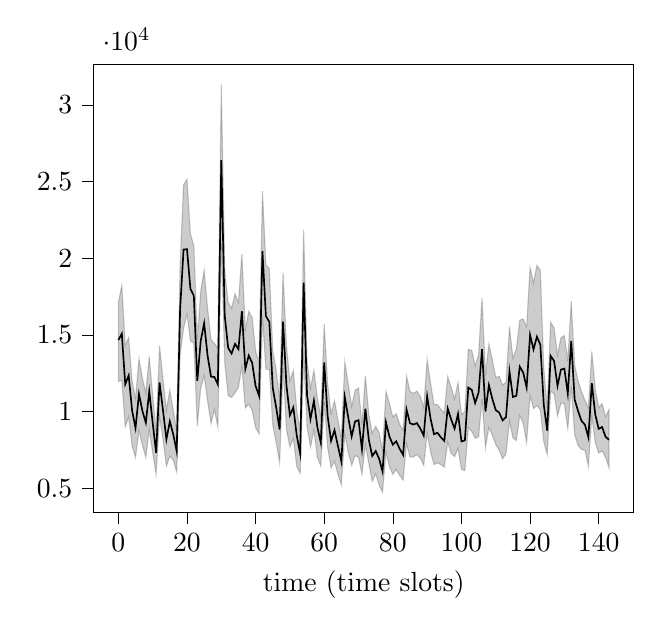
\begin{tikzpicture}

\begin{axis}[
tick align=outside,
tick pos=left,
x grid style={white!69.0196078431373!black},
xlabel={time (time slots)},
xmin=-7.15, xmax=150.15,
xtick style={color=black},
y grid style={white!69.0196078431373!black},
% ylabel={load},
ymin=3418.45972222222, ymax=32663.4569444444,
ytick style={color=black}
]
\path [draw=black, fill=black, opacity=0.2]
(axis cs:0,17116.9305555556)
--(axis cs:0,11964.8888888889)
--(axis cs:1,12054.2777777778)
--(axis cs:2,9012.73611111111)
--(axis cs:3,9655.95833333333)
--(axis cs:4,7755.43055555556)
--(axis cs:5,7020.20833333333)
--(axis cs:6,8786.80555555555)
--(axis cs:7,7818.33333333333)
--(axis cs:8,7014.68055555556)
--(axis cs:9,8829.77777777778)
--(axis cs:10,7319.91666666667)
--(axis cs:11,5903.77777777778)
--(axis cs:12,9645.61111111111)
--(axis cs:13,8199.40277777778)
--(axis cs:14,6452.55555555556)
--(axis cs:15,7092.33333333333)
--(axis cs:16,6836.31944444444)
--(axis cs:17,6055.90277777778)
--(axis cs:18,13669.4722222222)
--(axis cs:19,15432.4444444444)
--(axis cs:20,16375.9444444444)
--(axis cs:21,14607.625)
--(axis cs:22,14468.9444444444)
--(axis cs:23,9076.29166666667)
--(axis cs:24,11530.0694444444)
--(axis cs:25,12346.8472222222)
--(axis cs:26,10704.6527777778)
--(axis cs:27,9222.41666666667)
--(axis cs:28,10122.7916666667)
--(axis cs:29,8991.61111111111)
--(axis cs:30,20976.9861111111)
--(axis cs:31,13212.2222222222)
--(axis cs:32,11048.1527777778)
--(axis cs:33,10929.5972222222)
--(axis cs:34,11217.2916666667)
--(axis cs:35,11593.4722222222)
--(axis cs:36,12979.7777777778)
--(axis cs:37,10230.625)
--(axis cs:38,10489.1388888889)
--(axis cs:39,10087.4583333333)
--(axis cs:40,8960.02777777778)
--(axis cs:41,8552.19444444445)
--(axis cs:42,16202.6805555556)
--(axis cs:43,12761.1666666667)
--(axis cs:44,12758.3333333333)
--(axis cs:45,9132.04166666667)
--(axis cs:46,7981.41666666667)
--(axis cs:47,6646.65277777778)
--(axis cs:48,12828.4583333333)
--(axis cs:49,8828.31944444444)
--(axis cs:50,7685.93055555556)
--(axis cs:51,8245.5)
--(axis cs:52,6433.15277777778)
--(axis cs:53,5968.34722222222)
--(axis cs:54,13664.4166666667)
--(axis cs:55,9011.09722222222)
--(axis cs:56,7691.25)
--(axis cs:57,8794.61111111111)
--(axis cs:58,7007.95833333333)
--(axis cs:59,6459.94444444444)
--(axis cs:60,10622.2638888889)
--(axis cs:61,7660.73611111111)
--(axis cs:62,6323.77777777778)
--(axis cs:63,6754.55555555556)
--(axis cs:64,5910.80555555556)
--(axis cs:65,5226.05555555556)
--(axis cs:66,8551.40277777778)
--(axis cs:67,7326.44444444444)
--(axis cs:68,6502.95833333333)
--(axis cs:69,7121.48611111111)
--(axis cs:70,7027.22222222222)
--(axis cs:71,5904.65277777778)
--(axis cs:72,7855.11111111111)
--(axis cs:73,6603.43055555556)
--(axis cs:74,5450.11111111111)
--(axis cs:75,5943.66666666667)
--(axis cs:76,5207.43055555555)
--(axis cs:77,4747.77777777778)
--(axis cs:78,7363.48611111111)
--(axis cs:79,6428.56944444444)
--(axis cs:80,5906.76388888889)
--(axis cs:81,6218.52777777778)
--(axis cs:82,5838.44444444444)
--(axis cs:83,5538.66666666667)
--(axis cs:84,7896.38888888889)
--(axis cs:85,7025.97222222222)
--(axis cs:86,7045.97222222222)
--(axis cs:87,7201.33333333333)
--(axis cs:88,6971.18055555556)
--(axis cs:89,6493.80555555556)
--(axis cs:90,8615.88888888889)
--(axis cs:91,7386.13888888889)
--(axis cs:92,6545.11111111111)
--(axis cs:93,6658.48611111111)
--(axis cs:94,6547.47222222222)
--(axis cs:95,6380.13888888889)
--(axis cs:96,8005.23611111111)
--(axis cs:97,7276.26388888889)
--(axis cs:98,7055.58333333333)
--(axis cs:99,7617.31944444444)
--(axis cs:100,6232.43055555556)
--(axis cs:101,6159.36111111111)
--(axis cs:102,8960.22222222222)
--(axis cs:103,8711.04166666667)
--(axis cs:104,8263.31944444445)
--(axis cs:105,8348.01388888889)
--(axis cs:106,10818.2222222222)
--(axis cs:107,7648.38888888889)
--(axis cs:108,8972.33333333333)
--(axis cs:109,8468.47222222222)
--(axis cs:110,7852.55555555556)
--(axis cs:111,7497.34722222222)
--(axis cs:112,6928.5)
--(axis cs:113,7252.63888888889)
--(axis cs:114,9378.43055555556)
--(axis cs:115,8297)
--(axis cs:116,8106.73611111111)
--(axis cs:117,9748.70833333333)
--(axis cs:118,9231.13888888889)
--(axis cs:119,7978.40277777778)
--(axis cs:120,11053.0555555556)
--(axis cs:121,10206.1944444444)
--(axis cs:122,10390.3055555556)
--(axis cs:123,10123.75)
--(axis cs:124,8028.80555555556)
--(axis cs:125,7208.296875)
--(axis cs:126,11329.625)
--(axis cs:127,11166.625)
--(axis cs:128,9715.578125)
--(axis cs:129,10546.75)
--(axis cs:130,10523.828125)
--(axis cs:131,8875.65625)
--(axis cs:132,11644.484375)
--(axis cs:133,8505.1875)
--(axis cs:134,7793.359375)
--(axis cs:135,7532.859375)
--(axis cs:136,7480.828125)
--(axis cs:137,6434.96875)
--(axis cs:138,9670.984375)
--(axis cs:139,8012.515625)
--(axis cs:140,7293.390625)
--(axis cs:141,7434.4375)
--(axis cs:142,7025.125)
--(axis cs:143,6346.390625)
--(axis cs:143,10129.71875)
--(axis cs:143,10129.71875)
--(axis cs:142,9676.59375)
--(axis cs:141,10524.78125)
--(axis cs:140,10269.640625)
--(axis cs:139,11478)
--(axis cs:138,13931.234375)
--(axis cs:137,10252.5)
--(axis cs:136,10733.765625)
--(axis cs:135,11309.75)
--(axis cs:134,12009.234375)
--(axis cs:133,13015.296875)
--(axis cs:132,17229.75)
--(axis cs:131,13287.25)
--(axis cs:130,14962.25)
--(axis cs:129,14819.78125)
--(axis cs:128,13696.703125)
--(axis cs:127,15447.25)
--(axis cs:126,15841.625)
--(axis cs:125,10279.59375)
--(axis cs:124,12846.8333333333)
--(axis cs:123,19212.3055555556)
--(axis cs:122,19544.4027777778)
--(axis cs:121,18392.25)
--(axis cs:120,19409.3055555556)
--(axis cs:119,15535.9027777778)
--(axis cs:118,16042.5694444444)
--(axis cs:117,15970.6805555556)
--(axis cs:116,14088.1805555556)
--(axis cs:115,13482.5416666667)
--(axis cs:114,15552.5833333333)
--(axis cs:113,11920.0555555556)
--(axis cs:112,11729.75)
--(axis cs:111,12308.6527777778)
--(axis cs:110,12228.3888888889)
--(axis cs:109,13382.4027777778)
--(axis cs:108,14407.9861111111)
--(axis cs:107,12375.4166666667)
--(axis cs:106,17433.8888888889)
--(axis cs:105,13693.6805555556)
--(axis cs:104,12989.5416666667)
--(axis cs:103,13991.9027777778)
--(axis cs:102,14063.0833333333)
--(axis cs:101,10008.875)
--(axis cs:100,9809.08333333333)
--(axis cs:99,11900.0555555556)
--(axis cs:98,10812.5555555556)
--(axis cs:97,11585.3333333333)
--(axis cs:96,12279.0416666667)
--(axis cs:95,9906.125)
--(axis cs:94,10150.1111111111)
--(axis cs:93,10470.5416666667)
--(axis cs:92,10463.9722222222)
--(axis cs:91,11845.5694444444)
--(axis cs:90,13397.0416666667)
--(axis cs:89,10280.0416666667)
--(axis cs:88,11008.2083333333)
--(axis cs:87,11339.8888888889)
--(axis cs:86,11188.5277777778)
--(axis cs:85,11321.7638888889)
--(axis cs:84,12313.8333333333)
--(axis cs:83,8794.88888888889)
--(axis cs:82,9163.11111111111)
--(axis cs:81,9860.5)
--(axis cs:80,9660.40277777778)
--(axis cs:79,10537.2361111111)
--(axis cs:78,11311.3333333333)
--(axis cs:77,7470.22222222222)
--(axis cs:76,8634)
--(axis cs:75,9037.22222222222)
--(axis cs:74,8596.81944444444)
--(axis cs:73,9800.125)
--(axis cs:72,12344.9166666667)
--(axis cs:71,9146.58333333333)
--(axis cs:70,11543.8888888889)
--(axis cs:69,11397.5277777778)
--(axis cs:68,10343.0277777778)
--(axis cs:67,11828.6527777778)
--(axis cs:66,13244.1944444444)
--(axis cs:65,8261.26388888889)
--(axis cs:64,9459.20833333333)
--(axis cs:63,10704.3194444444)
--(axis cs:62,9876.38888888889)
--(axis cs:61,11808.9722222222)
--(axis cs:60,15698.8333333333)
--(axis cs:59,9637.45833333333)
--(axis cs:58,10895)
--(axis cs:57,12690.6388888889)
--(axis cs:56,11528.25)
--(axis cs:55,13294.2916666667)
--(axis cs:54,21871.0833333333)
--(axis cs:53,8658.65277777778)
--(axis cs:52,10131.8055555556)
--(axis cs:51,12667.9305555556)
--(axis cs:50,12018.3472222222)
--(axis cs:49,14292.4166666667)
--(axis cs:48,19054.9861111111)
--(axis cs:47,10845.2916666667)
--(axis cs:46,12746.5694444444)
--(axis cs:45,13975.5972222222)
--(axis cs:44,19320.5416666667)
--(axis cs:43,19579.6111111111)
--(axis cs:42,24378.2777777778)
--(axis cs:41,13245)
--(axis cs:40,13934.7638888889)
--(axis cs:39,16127.5277777778)
--(axis cs:38,16545.0138888889)
--(axis cs:37,15335.5277777778)
--(axis cs:36,20299.0972222222)
--(axis cs:35,17130.4027777778)
--(axis cs:34,17681.1111111111)
--(axis cs:33,16743.7638888889)
--(axis cs:32,17108.6944444444)
--(axis cs:31,19181.125)
--(axis cs:30,31334.1388888889)
--(axis cs:29,14127.0555555556)
--(axis cs:28,14451.875)
--(axis cs:27,14691.875)
--(axis cs:26,16738.0972222222)
--(axis cs:25,19246.9722222222)
--(axis cs:24,17847.2222222222)
--(axis cs:23,14675.625)
--(axis cs:22,20811.2361111111)
--(axis cs:21,21586.375)
--(axis cs:20,25151.6388888889)
--(axis cs:19,24798.5694444444)
--(axis cs:18,19584.2222222222)
--(axis cs:17,8797.94444444444)
--(axis cs:16,10067.8194444444)
--(axis cs:15,11404.3333333333)
--(axis cs:14,10102.2361111111)
--(axis cs:13,12136.4027777778)
--(axis cs:12,14297.2361111111)
--(axis cs:11,8668.77777777778)
--(axis cs:10,11091.4583333333)
--(axis cs:9,13600.8472222222)
--(axis cs:8,11207.2361111111)
--(axis cs:7,12166.5972222222)
--(axis cs:6,13465.8472222222)
--(axis cs:5,10846.2638888889)
--(axis cs:4,12015.0555555556)
--(axis cs:3,14825.3888888889)
--(axis cs:2,14342.4444444444)
--(axis cs:1,18239.4722222222)
--(axis cs:0,17116.9305555556)
--cycle;

\addplot [semithick]
table {%
0 14672.2222222222
1 15082.3333333333
2 11790.1111111111
3 12356.5555555556
4 10071.8888888889
5 8929.77777777778
6 11160.5555555556
7 10051.1111111111
8 9278.33333333333
9 11316.2222222222
10 9272.88888888889
11 7304.55555555556
12 11899.5555555556
13 10095.1111111111
14 8193.66666666667
15 9365.33333333333
16 8515.44444444445
17 7415.55555555556
18 16695.4444444444
19 20574.4444444444
20 20595.5555555556
21 18009
22 17552.5555555556
23 12012.5555555556
24 14611.4444444444
25 15760.3333333333
26 13659.1111111111
27 12284.5555555556
28 12256.3333333333
29 11774.1111111111
30 26411
31 16250.4444444444
32 14160.5555555556
33 13789.6666666667
34 14420.4444444444
35 14078.2222222222
36 16547.5555555556
37 12778.1111111111
38 13651.3333333333
39 13176.5555555556
40 11666.8888888889
41 11047.3333333333
42 20463.1111111111
43 16231.1111111111
44 15852.1111111111
45 11542.4444444444
46 10270.8888888889
47 8837.33333333333
48 15872.4444444444
49 11676.8888888889
50 9762.66666666667
51 10272.6666666667
52 8427.22222222222
53 7248.44444444444
54 18410.6666666667
55 11059.2222222222
56 9519
57 10722
58 8988.88888888889
59 7974.77777777778
60 13207.7777777778
61 9693.77777777778
62 8095.55555555556
63 8787.44444444445
64 7761.33333333333
65 6746.88888888889
66 10943.5555555556
67 9627.77777777778
68 8384
69 9361.88888888889
70 9442.44444444445
71 7538.22222222222
72 10194.4444444444
73 8157.66666666667
74 7104.88888888889
75 7431.88888888889
76 6929.55555555556
77 6095.88888888889
78 9306.33333333333
79 8377.44444444445
80 7848.55555555556
81 8061.88888888889
82 7568.22222222222
83 7182.66666666667
84 10142.1111111111
85 9244.33333333333
86 9157.55555555555
87 9250.55555555555
88 8903.66666666667
89 8438.88888888889
90 11003.8888888889
91 9540.66666666667
92 8528.22222222222
93 8619.11111111111
94 8324.44444444445
95 8092.33333333333
96 10202.2222222222
97 9488.77777777778
98 8891.77777777778
99 9852.77777777778
100 8061.33333333333
101 8120.11111111111
102 11568
103 11423.4444444444
104 10560
105 11250.3333333333
106 14069
107 10012.3333333333
108 11732.5555555556
109 10837.7777777778
110 10095.7777777778
111 9936.44444444445
112 9430.22222222222
113 9646.77777777778
114 12626
115 10957.2222222222
116 11034.8888888889
117 12931.3333333333
118 12550.4444444444
119 11570.7777777778
120 15004
121 14053.2222222222
122 14886.7777777778
123 14360.6666666667
124 10444.2222222222
125 8757.125
126 13635.75
127 13310.5
128 11687.75
129 12740.625
130 12804.5
131 11172.5
132 14607.5
133 10795.125
134 10031
135 9395.75
136 9144.75
137 8326.125
138 11856.625
139 9819.5
140 8878.5
141 8997.625
142 8360.875
143 8164.75
};
\end{axis}

\end{tikzpicture}
}
    \caption{Alibaba}\label{fig:alibaba:histogram}
    \end{subfigure}
    \caption{LANL Mustang, Microsoft Fiddle, and Alibaba traces. The figures display the average number of job arrivals throughout a day. The interquartile range is shown as the shaded region.}
\end{figure}

\begin{figure}
    \begin{subfigure}[b]{.345\linewidth}
    \resizebox{\textwidth}{!}{% This file was created by tikzplotlib v0.9.9.
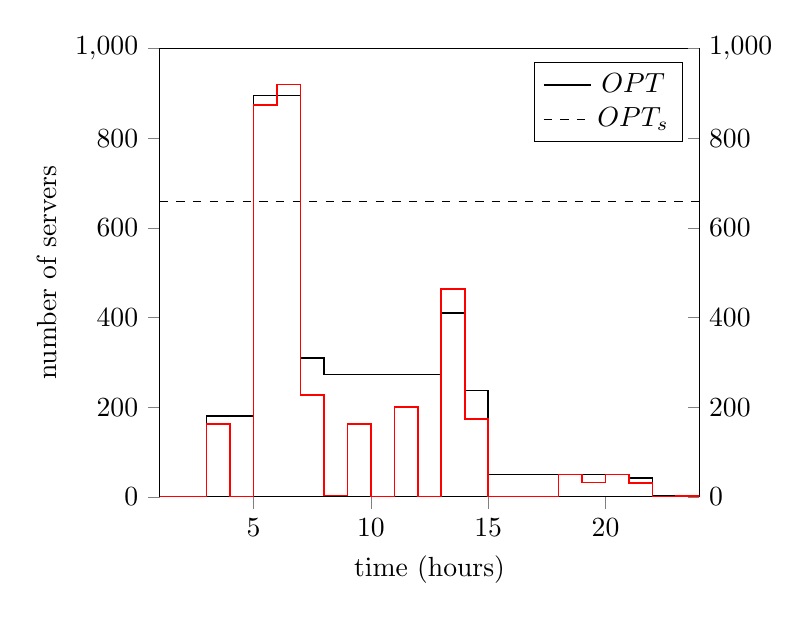
\begin{tikzpicture}

\begin{axis}[
legend pos=north east,
tick align=outside,
tick pos=left,
% x grid style={white!69.0196078431373!black},
xlabel={time (hours)},
xmin=1, xmax=24,
% xtick style={color=black},
% y grid style={white!69.0196078431373!black},
ylabel={number of servers},
ymin=0, ymax=1000,
% ytick style={color=black}
]
\addplot [semithick, black, const plot mark left]
table {%
1 1
2 1
3 181
4 181
5 895
6 895
7 309
8 273
9 273
10 273
11 273
12 273
13 410
14 237
15 50
16 50
17 50
18 50
19 50
20 50
21 42
22 2
23 2
24 1
};
\addlegendentry{$OPT$}

\draw[dashed, color=black] (axis cs:\pgfkeysvalueof{/pgfplots/xmin},659) -- (axis cs:\pgfkeysvalueof{/pgfplots/xmax},659);
\addlegendimage{dashed, color=black}
\addlegendentry{$OPT_s$}
\end{axis}

\begin{axis}[
axis y line*=right,
axis x line=none,
xmin=1, xmax=24,
ymin=0, ymax=1000,
% ylabel=load
]
\addplot [semithick, red, const plot mark left]
table {%
1 1
2 0
3 163
4 1
5 874
6 920
7 227
8 3
9 162
10 1
11 201
12 0
13 464
14 174
15 0
16 0
17 1
18 50
19 32
20 50
21 31
22 0
23 2
24 1
};
\end{axis}

\end{tikzpicture}
}
    \caption{LANL Mustang}\label{fig:los_alamos:schedule}
    \end{subfigure}
    \begin{subfigure}[b]{.305\linewidth}
    \resizebox{\textwidth}{!}{% This file was created by tikzplotlib v0.9.9.
\begin{tikzpicture}

\begin{axis}[
legend pos=north east,
axis y line*=right,
axis x line=none,
xmin=1, xmax=24,
ymin=-10, ymax=200,
% ylabel=load
]
\addplot [semithick, red, const plot mark left, name path=A]
table {%
1 32
2 43
3 42
4 16
5 29
6 9
7 9
8 13
9 12
10 15
11 22
12 10
13 14
14 121
15 22
16 25
17 122
18 12
19 27
20 8
21 16
22 115
23 27
24 23
};
\addlegendentry{load}

\addplot+[draw=none,domain=0:24,name path=B] {-10000};
\addplot+[red!5] fill between[of=A and B];
\end{axis}

\begin{axis}[
legend pos=north west,
tick align=outside,
tick pos=left,
% x grid style={white!69.0196078431373!black},
xlabel={time (hours)},
xmin=1, xmax=24,
% xtick style={color=black},
% y grid style={white!69.0196078431373!black},
% ylabel={number of servers},
ymin=-1.5, ymax=42,
% ytick style={color=black}
]
\addplot [semithick, black, const plot mark left]
table {%
1 9
2 13
3 0
4 0
5 0
6 0
7 0
8 0
9 0
10 0
11 0
12 0
13 0
14 34
15 34
16 34
17 34
18 29
19 29
20 29
21 29
22 29
23 0
24 0
};
\addlegendentry{$OPT$ 2 GPUs}
\addplot [ultra thick, black, const plot mark left]
table {%
1 4
2 4
3 4
4 4
5 4
6 4
7 4
8 4
9 4
10 4
11 4
12 4
13 4
14 12
15 12
16 12
17 12
18 12
19 12
20 12
21 12
22 12
23 4
24 4
};
\addlegendentry{$OPT$ 8 GPUs}

\draw[dashed, color=black] (axis cs:\pgfkeysvalueof{/pgfplots/xmin},0) -- (axis cs:\pgfkeysvalueof{/pgfplots/xmax},0);
\addlegendimage{dashed, color=black}
\addlegendentry{$OPT_s$ 2 GPUs}
\draw[dashed, ultra thick, color=black] (axis cs:\pgfkeysvalueof{/pgfplots/xmin},17) -- (axis cs:\pgfkeysvalueof{/pgfplots/xmax},17);
\addlegendimage{dashed, ultra thick, color=black}
\addlegendentry{$OPT_s$ 8 GPUs}
\end{axis}

\end{tikzpicture}
}
    \caption{Microsoft Fiddle}\label{fig:microsoft:schedule}
    \end{subfigure}
    \begin{subfigure}[b]{.335\linewidth}
    \resizebox{\textwidth}{!}{% This file was created by tikzplotlib v0.9.9.
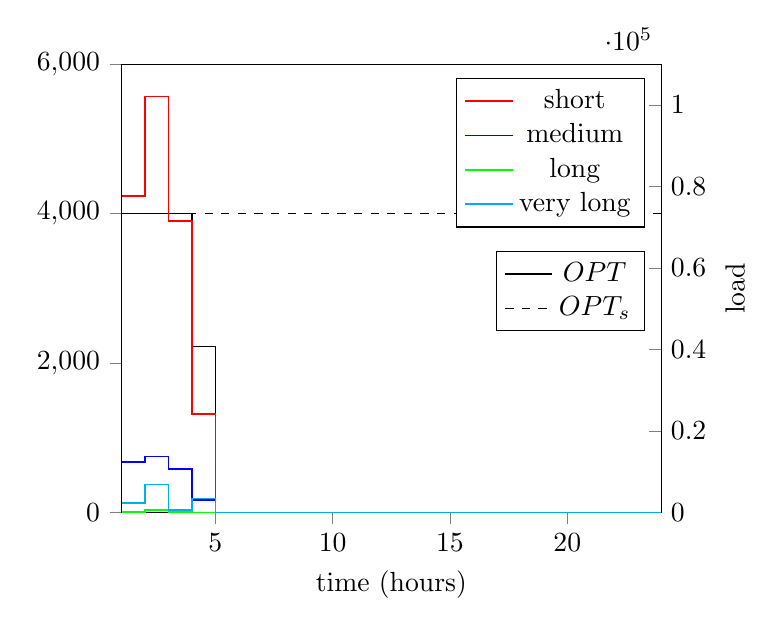
\begin{tikzpicture}

\begin{axis}[
legend style={at={(axis cs:23.3,3500)},anchor=north east},
tick align=outside,
tick pos=left,
% x grid style={white!69.0196078431373!black},
xlabel={time (hours)},
xmin=1, xmax=24,
% xtick style={color=black},
% y grid style={white!69.0196078431373!black},
% ylabel={proportion of iterations},
ymin=0, ymax=6000,
% ytick style={color=black}
]
\addplot [semithick, black, const plot mark left]
table {%
1 4000
2 4000
3 4000
4 2223
5 1
6 1
7 1
8 1
9 1
10 1
11 1
12 1
13 1
14 0
15 0
16 0
17 0
18 0
19 0
20 0
21 0
22 1
23 1
24 1
};
\addlegendentry{$OPT$}

\draw[dashed, color=black] (axis cs:\pgfkeysvalueof{/pgfplots/xmin},4000) -- (axis cs:\pgfkeysvalueof{/pgfplots/xmax},4000);
\addlegendimage{dashed, color=black}
\addlegendentry{$OPT_s$}
\end{axis}

\begin{axis}[
legend pos=north east,
axis y line*=right,
axis x line=none,
xmin=1, xmax=24,
ymin=0, ymax=110000,
ylabel=load
]
\addplot [semithick, red, const plot mark left]
table {%
1 77680
2 102062
3 71522
4 24183
5 2
6 4
7 0
8 2
9 1
10 0
11 1
12 3
13 1
14 0
15 0
16 0
17 0
18 0
19 0
20 0
21 0
22 1
23 0
24 1
};
\addlegendentry{short}
\addplot [semithick, blue, const plot mark left]
table {%
1 12362
2 13705
3 10655
4 3024
5 0
6 0
7 0
8 0
9 0
10 0
11 0
12 0
13 0
14 0
15 0
16 0
17 0
18 0
19 0
20 0
21 0
22 0
23 0
24 0
};
\addlegendentry{medium}
\addplot [semithick, green, const plot mark left]
table {%
1 105
2 628
3 164
4 33
5 0
6 0
7 0
8 0
9 0
10 0
11 0
12 0
13 0
14 0
15 0
16 0
17 0
18 0
19 0
20 0
21 0
22 0
23 0
24 0
};
\addlegendentry{long}
\addplot [semithick, cyan, const plot mark left]
table {%
1 2319
2 6870
3 550
4 3440
5 0
6 0
7 0
8 0
9 0
10 0
11 0
12 0
13 0
14 0
15 0
16 0
17 0
18 0
19 0
20 0
21 0
22 0
23 0
24 0
};
\addlegendentry{very long}
\end{axis}

\end{tikzpicture}
}
    \caption{Alibaba}\label{fig:alibaba:schedule}
    \end{subfigure}
    \caption{Optimal dynamic and static offline schedules for the last day of the LANL Mustang, Microsoft Fiddle, and the second to last day of the Alibaba trace. The left y axis shows the number of servers of the static and dynamic offline optima at a given time (black). The right y axis shows the number of jobs (i.e., the load) at a given time (red).}
\end{figure}

\paragraph{} We have seen traces from very different real-world use cases. The Microsoft Fiddle trace is based on a heterogeneous server architecture, and the Alibaba trace receives heterogeneous loads. The PMR and valley lengths of the days used in our analysis are shown in \cref{tab:pmr_vl}. Interestingly, as shown in \cref{tab:traces}, their TPMR, peak distances, and valley lengths are mostly similar.

\subsection{Assumptions}

We impose a couple of assumptions to simplify our analysis. First, and already mentioned, our analysis is inherently limited by the traces we used as a basis for our experiments. While we examine a wide variety of traces, the high variability in traces indicates they are a fundamental limitation to any estimation of real-world performance.

Another common limitation of models is that the interarrival times of jobs are on the order of seconds or smaller~\cite{Amvrosiadis2018}. However, this is not a limitation of our analysis as we are using a general Poisson process with an appropriate mean arrival rate in our delay model.

In the context of high-performance computing, jobs typically have a \emph{gang scheduling}\index{gang scheduling} requirement, i.e., a requirement that related jobs are processed simultaneously even though they are run on different hardware~\cite{Amvrosiadis2018}. For simplification, we assume this requirement always to be satisfied. However, this is not a substantial limitation as the scheduling of jobs within a time slot is not determined by the discussed algorithms and instead left to the server operator. Nevertheless, in principle, the gang scheduling requirement may render some schedules infeasible if the processing time on servers exceeds the length of a time slot when gang scheduling constraints are considered.

There are also some limitations resulting from the design of our model. As was mentioned previously, we assume that the jobs arrive at the beginning of a new time slot rather than at random times throughout the time slot. Moreover, we assumed that for every job, a server type exists that can process this job within one time slot. In other words, there exists no job running longer than $\delta$. We have seen in \cref{section:case_studies:method:traces} that this assumption is violated in most practical scenarios. In \cref{section:application:dynamic_duration}, we described how this assumption can be removed. The same approach can also be used to remove the assumption that jobs must arrive at the beginning of a time slot.

\subsection{Alternatives to Right-Sizing Data Centers}\label{section:case_studies:method:alternatives}

To determine the benefit of dynamically right-sizing data centers, we must first describe the alternative strategies to managing a data center. We will then use these approaches as a point of reference in our analysis.

Most data centers are statically provisioned; that is, the configuration of active servers is only changed rarely (often manually) and remains constant during most periods~\cite{Whitney2014}. To support the highest loads, the data centers are peak-provisioned, i.e., the number of servers is chosen such that they suffice to process all jobs even during times where most jobs arrive. Moreover, as a safety measure, data centers are typically provisioned to handle much higher loads than the loads encountered in practice~\cite{Whitney2014}.

\begin{table}
    \centering
    \begin{tabularx}{\textwidth}{>{\bfseries}l|X|X|X}
        characteristic & LANL Mustang & Microsoft Fiddle & Alibaba \\\hline
        duration & 5 years & 30 days & 8 days \\
        number of jobs & 20 million & 120 thousand & 14 million \\
        median interarrival time & 0 seconds & 8 seconds & 0 seconds \\
        PMR & 621.94 & 89.43 & 3.93 \\
        TPMR & 2.5 & 1.68 & 1.77 \\
        mean peak distance & 100 minutes & 105 minutes & 89 minutes \\
        mean valley length & 120 minutes & 115 minutes & 74 minutes \\
        diurnal pattern & yes & - & yes \\
    \caption{Characteristics of the LANL Mustang, Microsoft Fiddle, and Alibaba traces.}
    \end{tabularx}
    \label{tab:traces}
\end{table}

Naturally, traces with a high PMR or long valleys are more likely to benefit from alternatives to static provisioning. Therefore another widely used alternative is \emph{valley filling}\index{valley filling}, which aims to schedule lower priority jobs (i.e., some batch jobs) during valleys. In an ideal scenario, this approach can achieve $\text{PMR} \approx 1$, which would allow for efficient static provisioning. Crucially, this approach requires a large number of low-priority jobs which may be processed with a significant delay (requiring a considerable minimum perceptible delay $\delta_i$ for a large number of jobs of type $i$), and thus in most cases, valleys cannot be eliminated entirely. \citeauthor*{Lin2011}~\cite{Lin2011} showed that dynamic-right sizing can be combined with valley filling to achieve a significant cost reduction. The optimal balancing of dynamic right-sizing and valley filling is mainly determined by the change to the PMR. \citeauthor*{Lin2011}~\cite{Lin2011} showed that cost savings of 20\% are possible with a PMR of 2 and a PMR of approximately 1.3 can still achieve cost savings of more than 5\%. Generally, the cost reduction vanishes once the PMR approaches $1$, which may happen between 30\% to 70\% mean background load~\cite{Lin2011}. The results when dynamic right-sizing is used together with valley filling can be estimated from previous results.

\subsection{Performance Metrics}

Let $OPT$ denote the dynamic offline optimum and $OPT_s$ denote the static offline optimum. In our analysis, the \emph{normalized cost}\index{normalized cost} of an online algorithm is the ratio of the obtained cost and the dynamic optimal offline cost, i.e. $NC(ALG) = c(ALG) / c(OPT)$. Further, we base our estimated \emph{cost reduction}\index{cost reduction} on an optimal offline static provisioning: \begin{align*}
    CR(ALG) = \frac{c(OPT_s) - c(ALG)}{c(OPT_s)}.
\end{align*} Note that this definition is similar to the definition of regret, but expressed relative to the overall cost. We refer to $SDR = c(OPT_s) / c(OPT)$ as the \emph{static/dynamic ratio}\index{static/dynamic ratio}, which is closely related to the \emph{potential cost reduction}\index{potential cost reduction} $PCR = CR(OPT)$.

\subsection{Previous Results}

\citeauthor*{Lin2011}~\cite{Lin2011} showed that the cost reduction is directly proportional to the PMR and inversely proportional to the normalized switching cost. Additionally, \citeauthor*{Lin2011}~\cite{Lin2011} showed that, as one would expect, the possible cost reduction decreases as the delay cost assumes a more significant fraction of the overall hitting costs. In practice, this can be understood as the effect of making the model more conservative.

\begin{table}
    \centering
    \begin{tabularx}{\textwidth}{>{\bfseries}l|c|c}
        trace & PMR & mean valley length (hours) \\\hline
        Facebook 2009-0 & 2.115 & 2.565 \\
        Facebook 2009-1 & 1.913 & 1.522 \\
        Facebook 2010 & 1.549 & 1.435 \\
        LANL Mustang & 6.575 & 1.167 \\
        Microsoft Fiddle & 3.822 & 2.125 \\
        Alibaba & 1.339 & 2.792 \\
    \caption{PMR and mean valley length of the traces used in our analysis. Note that the valley lengths are typically shorter than the normalized switching cost of our model.}
    \end{tabularx}
    \label{tab:pmr_vl}
\end{table}

\subsection{Model Parameters}\label{section:case_studies:traces:model-parameters}

We now describe how we parametrized our model in our case studies. In our models, we strive to choose conservative estimates to under-estimate the cost savings from dynamically right-sizing data centers. This approach is similar to the study by \citeauthor*{Lin2011}~\cite{Lin2011}. \Cref{tab:model} gives an overview of the used parameters producing the results of subsequent sections.

\paragraph{Energy} We use the linear energy consumption model from \autoref{eq:energy_model:1} in our experiments. In their analysis, \citeauthor*{Lin2011}~\cite{Lin2011} choose energy cost and energy consumption such that the fixed energy cost (i.e., the energy cost of a server when idling) is $1$ and the dynamic energy cost is $0$ as, on most servers, the fixed costs dominate the dynamic costs~\cite{Clark2005}. We investigate this model and an alternative model. In the alternative model, we estimate the power consumption of a server with 1 kW during peak loads and with 500 W when idling to yield a conservative estimate (as cooling costs are included). According to the U.S. Energy Information Administration (EIA), the average cost of energy in the industrial sector in the United States during April 2021 was 6.77 cents per kilowatt-hour~\cite{EIA2021}. We use this as a conservative estimate as data centers typically use a more expensive portfolio of energy sources. If the actual carbon cost of the used energy were to be considered, which is the case in some data centers as discussed in \cref{section:application:operating_cost:energy}, energy costs are likely to be substantially higher.

\paragraph{Revenue Loss} According to measurements, a 500 ms increase in delay results in a revenue loss of 20\% or 0.04\%/ms~\cite{Lin2012, Hamilton2009}. Thus, scaling the delay measured in ms by 0.1 can be used as a slight over-approximation of revenue loss. \citeauthor*{Lin2011}~\cite{Lin2011} choose the minimal perceptible delay as 1.5 times the time to run a job, which is a very conservative estimate if valley filling is assumed a viable alternative. In our model, we choose the minimal perceptible delay as 2.5 times the time to run a job which is equivalent as we also added the processing time of a job to the delay. In the case of valley filling, jobs are typically processed with a much more significant delay. Similar to \citeauthor*{Lin2012}~\cite{Lin2012}, we also estimate a constant network delay of 10 ms.

\paragraph{Switching Cost} We mentioned in \cref{section:application:switching_cost} that in practice, the switching cost should be on the order of operating a server between an hour to several hours. To obtain a conservative estimate, we choose $\beta$ such that the normalized switching cost times the length of a time slot equals 4 hours.

\paragraph{Time Slot Length} We choose a time slot length of 1 hour. We further assume that the average processing time of jobs is $\delta / 2$ unless noted otherwise.

\begin{table}
    \centering
    \begin{tabularx}{\textwidth}{>{\bfseries}l|X|X}
        parameter & model 1 & model 2 \\\hline
        time slot length & 1 hour & 1 hour \\
        energy cost & $c=1$ & $c=0.0677$ \\
        energy consumption & $\Phi_{\text{min}}=1, \Phi_{\text{max}}=1$ & $\Phi_{\text{min}}=0.5, \Phi_{\text{max}}=1$ \\
        revenue loss & $\gamma = 0.1, \delta_i = 2.5 \eta_i$ & $\gamma = 0.1, \delta_i = 2.5 \eta_i$ \\
        normalized switching cost & 4 hours & 4 hours \\
    \caption{Models used in our case studies. $\eta_i$ is the processing time of jobs of type $i$.}
    \end{tabularx}
    \label{tab:model}
\end{table}

\section{Uni-Dimensional Algorithms}

The results of this section are based on the final day of the LANL Mustang, Facebook, and the second to last day of the Alibaba trace. We begin by discussing the general features of the traces. Then, we compare the uni-dimensional online algorithms with respect to their achieved normalized cost, cost reduction, and runtime.

\paragraph{Fractional vs. Integral Cost} For all traces, the ratio of the fractional and the integral costs is 1 for a precision of at least $10^{-3}$. This is not surprising due to the large number of servers used in each model.

\begin{figure}
    \begin{subfigure}[b]{.5\linewidth}
    \resizebox{\textwidth}{!}{% This file was created by tikzplotlib v0.9.9.
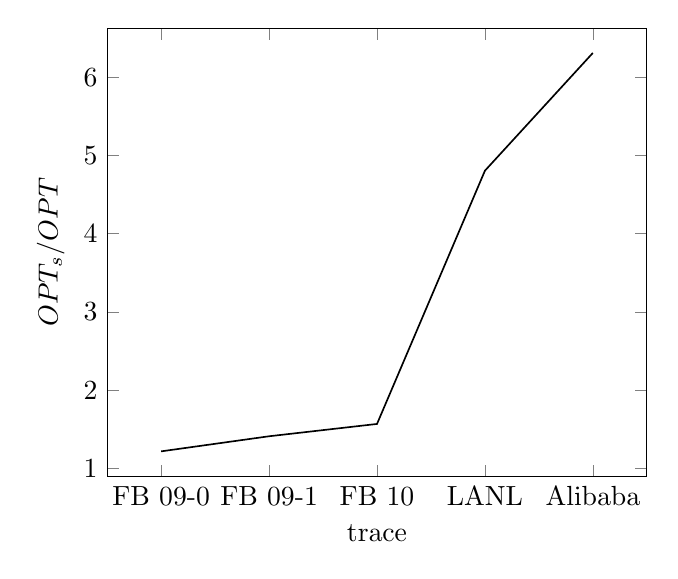
\begin{tikzpicture}

\begin{axis}[
% tick align=outside,
% tick pos=left,
% unbounded coords=jump,
% x grid style={white!69.0196078431373!black},
xlabel={trace},
xmin=-0.5, xmax=4.5,
% xtick style={color=black},
xtick={0,1,2,3,4},
xticklabels={FB 09-0,FB 09-1,FB 10,LANL,Alibaba},
% y grid style={white!69.0196078431373!black},
ylabel={$OPT_s / OPT$},
ymin=0.9, ymax=6.6244902738,
% ytick style={color=black}
]
% \draw[draw=black,fill=none] (axis cs:-0.4,0) rectangle (axis cs:0.4,1.571471378);
% \draw[draw=black,fill=none] (axis cs:0.6,0) rectangle (axis cs:1.4,1.414242315);
% \draw[draw=black,fill=none] (axis cs:1.6,0) rectangle (axis cs:2.4,1.221588301);
% \draw[draw=black,fill=none] (axis cs:2.6,0) rectangle (axis cs:3.4,4.805223659);
% \draw[draw=black,fill=none] (axis cs:3.6,0) rectangle (axis cs:4.4,6.309038356);
\addplot [semithick, black]
table {%
0 1.221588301
1 1.414242315
2 1.571471378
3 4.805223659
4 6.309038356
};
\end{axis}

\end{tikzpicture}
}
    \caption{Ratio of static and dynamic optima}
    \end{subfigure}
    \begin{subfigure}[b]{.5\linewidth}
    \resizebox{\textwidth}{!}{\pgfplotstableread{
X Y
2.115 1.1862049328218298
1.913 1.1540470009508415
1.549 1.0479312893570394
6.575 2.4294509720294735
3.822 1.9696643
1.339 1.068293057
}\a
\pgfplotstableread{
X Y
2.115 1.071842679781245
1.913 1.0433664197908732
1.549 1
6.575 1.9200838991565596
3.822 1.29969
1.339 1.011010843
}\b

\begin{tikzpicture}
\begin{axis}[
legend pos=south east,
ylabel={static/dynamic ratio},
xlabel={PMR}]
\addplot [only marks, blue, mark = o] table {\a};
\addlegendentry{model 1}
\addplot [only marks, red, mark = o] table {\b};
\addlegendentry{model 2}
\addplot [thick, blue] table[
    y={create col/linear regression={y=Y}}
] % compute a linear regression from the input table
{\a};
\addplot [thick, red] table[
    y={create col/linear regression={y=Y}}
] % compute a linear regression from the input table
{\b};
\end{axis}
\end{tikzpicture}}
    \caption{Correlation of the PMR and the static/dynamic ratio}\label{fig:case_studies:ud:opt_vs_opts:pmr}
    \end{subfigure}
    \caption{Ratio of static and dynamic offline optima for each trace. The LANL Mustang and Microsoft Fiddle traces have a significantly higher PMR than the remaining traces. Generally, we observe a strong correlation of PMR and the static/dynamic ratio.}\label{fig:case_studies:ud:opt_vs_opts}
\end{figure}

\begin{figure}
    \begin{subfigure}[b]{.49\linewidth}
    \resizebox{\textwidth}{!}{\pgfplotstableread{
X Y
1.1862049328218298 1.217963395
1.1862049328218298 1.073752054
1.1862049328218298 1.203176915
1.1862049328218298 1.213633822
1.1862049328218298 1.215964525
1.1540470009508415 1.264233547
1.1540470009508415 1.126679608
1.1540470009508415 1.177011887
1.1540470009508415 1.215947005
1.1540470009508415 1.215947005
1.0479312893570394 1.267149747
1.0479312893570394 1.144691647
1.0479312893570394 1.241611332
1.0479312893570394 1.246984786
1.0479312893570394 1.24775128
2.4294509720294735 1.793108632
2.4294509720294735 2.254697647
2.4294509720294735 1.243801312
2.4294509720294735 1.296624346
2.4294509720294735 1.294611567
1.068293057 1.220650656
1.068293057 1.082388905
1.068293057 1.165761722
1.068293057 1.149285464
1.068293057 1.149467892
}\a
\pgfplotstableread{
X Y
1.071842679781245 1.157784554
1.071842679781245 1.088245181
1.071842679781245 1.214821767
1.071842679781245 1.212900741
1.071842679781245 1.213648703
1.0433664197908732 1.205891207
1.0433664197908732 1.166348954
1.0433664197908732 1.153605888
1.0433664197908732 1.221498393
1.0433664197908732 1.222450113
1 1.042592762
1 1.002849673
1 1.07620715
1.9200838991565596 1.479166878
1.9200838991565596 1.895323607
1.9200838991565596 1.235296539
1.9200838991565596 1.363824754
1.9200838991565596 1.363368466
1.011010843 1.142369131
1.011010843 1.098736948
1.011010843 1.134416689
1.011010843 1.146620801
1.011010843 1.146662935
}\b

\begin{tikzpicture}
\begin{axis}[
legend pos=north west,
xlabel={static/dynamic ratio},
ylabel={normalized cost}]
\addplot [only marks, blue, mark = o] table {\a};
\addlegendentry{model 1}
\addplot [only marks, red, mark = o] table {\b};
\addlegendentry{model 2}
\addplot [thick, blue] table[
    y={create col/linear regression={y=Y}}
] % compute a linear regression from the input table
{\a};
\addplot [thick, red] table[
    y={create col/linear regression={y=Y}}
] % compute a linear regression from the input table
{\b};
\end{axis}
\end{tikzpicture}}
    \caption{Normalized cost}\label{fig:case_studies:ud:opt_vs_opts_against_normalized_cost}
    \end{subfigure}
    \begin{subfigure}[b]{.51\linewidth}
    \resizebox{\textwidth}{!}{% This file was created by tikzplotlib v0.9.9.
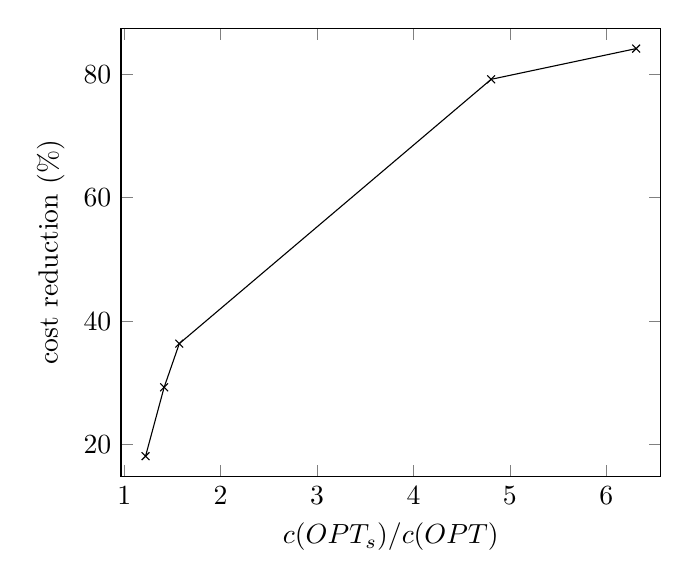
\begin{tikzpicture}

\begin{axis}[
% tick align=outside,
% tick pos=left,
% x grid style={white!69.0196078431373!black},
xlabel={$c(OPT_s) / c(OPT)$},
xmin=0.96721579825, xmax=6.56341085875,
% xtick style={color=black},
% y grid style={white!69.0196078431373!black},
ylabel={cost reduction (\%)},
ymin=14.8392859983333, ymax=87.437270835,
% ytick style={color=black}
]
\addplot[mark=x]
table {%
1.221588301 18.1391944
1.414242315 29.2892308571429
1.571471378 36.36242482
4.805223659 79.1618249666667
6.309038356 84.1373624333333
};
\end{axis}

\end{tikzpicture}
}
    \caption{Cost reduction}\label{fig:case_studies:ud:opt_vs_opts_against_mean_cost_reduction}
    \end{subfigure}
    \caption{Effect of the ratio of static and dynamic optima on the cost reduction and normalized cost achieved by the memoryless algorithm.}
\end{figure}

\paragraph{Dynamic vs. Static Cost} The dynamic and static costs differ significantly depending on the trace. The ratio of dynamic and static optimal costs for each trace is shown in \cref{fig:case_studies:ud:opt_vs_opts}.

\Cref{fig:case_studies:ud:opt_vs_opts_against_mean_cost_reduction} shows a strong positive correlation between the average cost reduction achieved by the memoryless algorithm and the ratio of the static and dynamic optima. As $OPT_s / OPT$ is directly linked to the PMR, this also indicates a strong correlation between cost reduction and the PMR. Even under our very conservative estimates of parameters, we achieve a significant cost reduction when the ratio of the static and dynamic offline optimum exceeds 1.5. Similar to \citeauthor*{Lin2011}~\cite{Lin2011}, we observe that cost savings increase rapidly as the PMR increases.

We also observe in \cref{fig:case_studies:ud:opt_vs_opts_against_normalized_cost} that as the static/dynamic ratio increases, the normalized costs achieved by the memoryless algorithm increases too but not as much as the potential energy savings, resulting in the observed significant cost reduction.

\begin{figure}
    \begin{subfigure}[b]{.3425\linewidth}
    \resizebox{\textwidth}{!}{% This file was created by tikzplotlib v0.9.9.
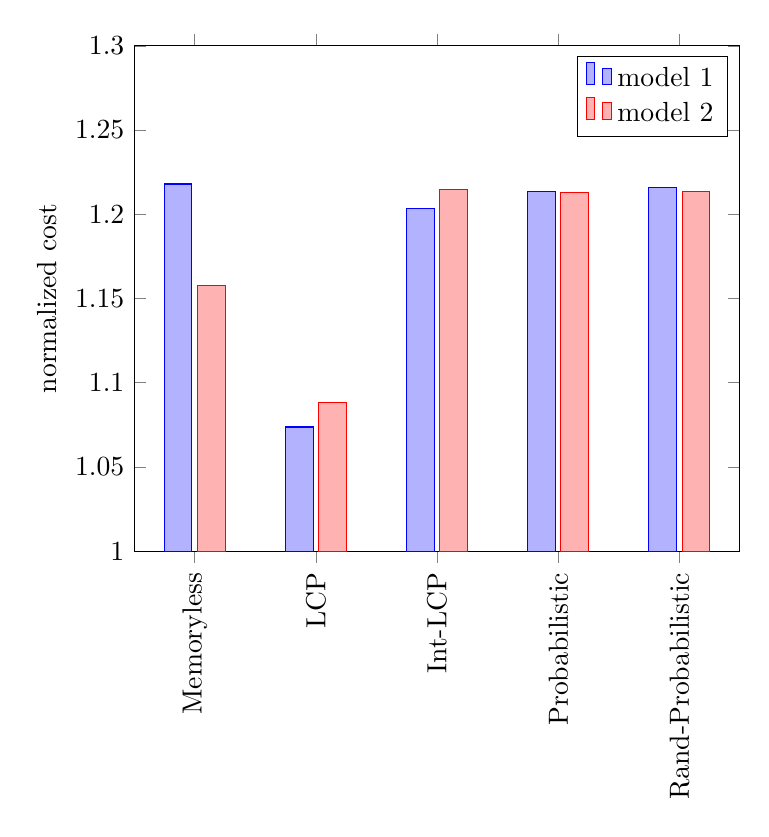
\begin{tikzpicture}

\begin{axis}[
ybar,
% bar width=0.5cm,
height=8cm,
% tick align=outside,
% tick pos=left,
% x grid style={white!69.0196078431373!black},
% xlabel={$OPT_s / OPT$},
xmin=-0.5, xmax=4.5,
xtick={0,1,2,3,4,5,6},
xticklabel style={rotate=90.0},
xticklabels={Memoryless,LCP,Int-LCP,Probabilistic,Rand-Probabilistic},
% xtick style={color=black},
% y grid style={white!69.0196078431373!black},
ylabel={normalized cost},
ymin=1, ymax=1.3,
% /pgf/number format/precision=5,
% ytick style={color=black}
]
\addplot
table {%
0 1.217963395
1 1.073752054
2 1.203176915
3 1.213633822
4 1.215964525
};
\addplot
table {%
0 1.157784554
1 1.088245181
2 1.214821767
3 1.212900741
4 1.213648703
};
\legend{model 1, model 2}
\end{axis}

\end{tikzpicture}
}
    \caption{Facebook 2009-0}
    \end{subfigure}
    \begin{subfigure}[b]{.32\linewidth}
    \resizebox{\textwidth}{!}{% This file was created by tikzplotlib v0.9.9.
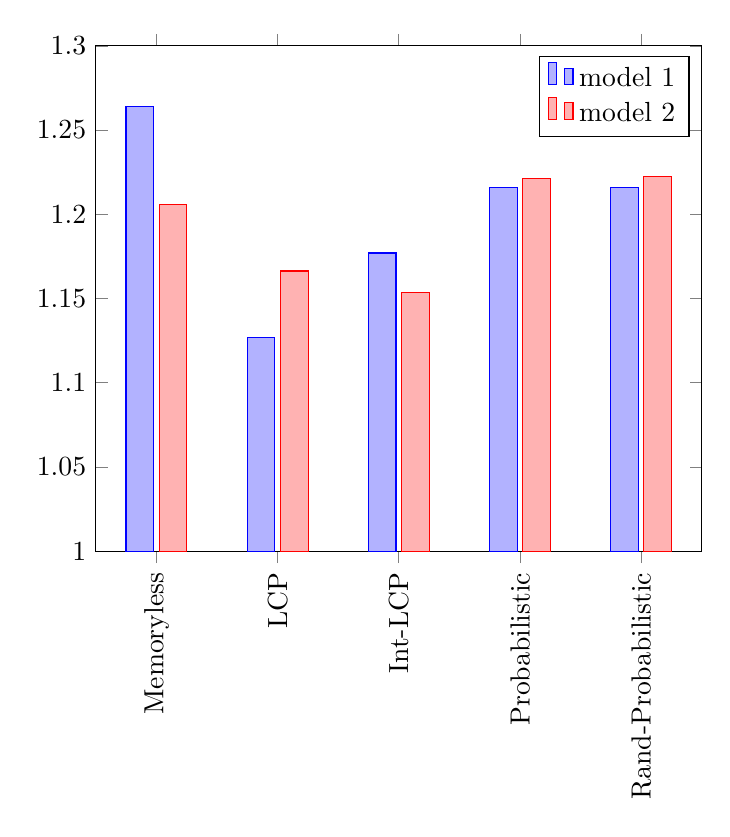
\begin{tikzpicture}

\begin{axis}[
ybar,
% bar width=0.5cm,
height=8cm,
% tick align=outside,
% tick pos=left,
% x grid style={white!69.0196078431373!black},
% xlabel={$OPT_s / OPT$},
xmin=-0.5, xmax=4.5,
xtick={0,1,2,3,4,5,6},
xticklabel style={rotate=90.0},
xticklabels={Memoryless,LCP,Int-LCP,Probabilistic,Rand-Probabilistic},
% xtick style={color=black},
% y grid style={white!69.0196078431373!black},
% ylabel={normalized cost},
ymin=1, ymax=1.3,
% /pgf/number format/precision=5,
% ytick style={color=black}
]
\addplot
table {%
0 1.264233547
1 1.126679608
2 1.177011887
3 1.215947005
4 1.215947005
};
\addplot
table {%
0 1.205891207
1 1.166348954
2 1.153605888
3 1.221498393
4 1.222450113
};
\legend{model 1, model 2}
\end{axis}

\end{tikzpicture}
}
    \caption{Facebook 2009-1}
    \end{subfigure}
    \begin{subfigure}[b]{.32\linewidth}
    \resizebox{\textwidth}{!}{% This file was created by tikzplotlib v0.9.9.
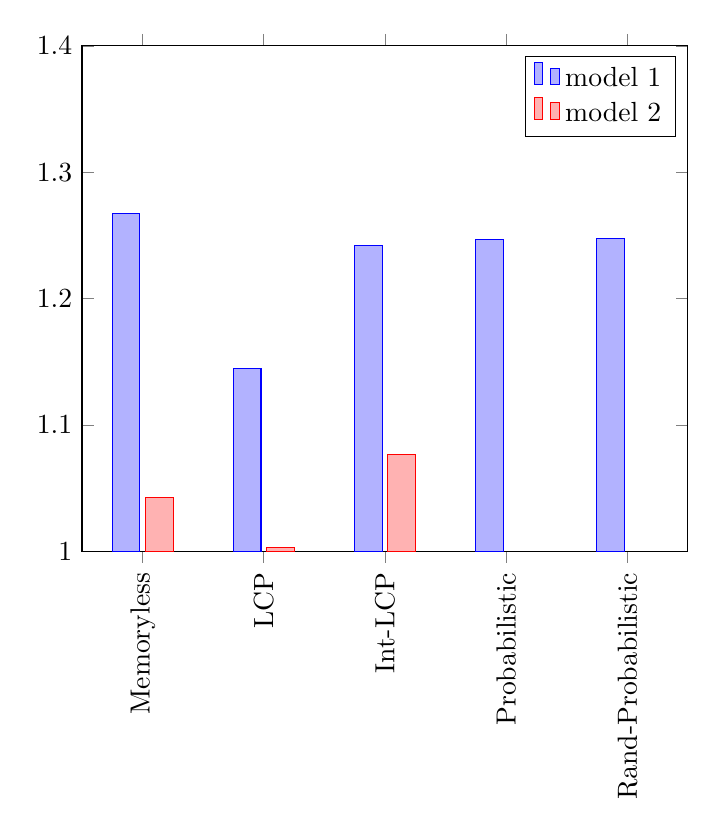
\begin{tikzpicture}

\begin{axis}[
ybar,
% bar width=0.5cm,
height=8cm,
% tick align=outside,
% tick pos=left,
% x grid style={white!69.0196078431373!black},
% xlabel={$OPT_s / OPT$},
xmin=-0.5, xmax=4.5,
xtick={0,1,2,3,4,5,6},
xticklabel style={rotate=90.0},
xticklabels={Memoryless,LCP,Int-LCP,Probabilistic,Rand-Probabilistic},
% xtick style={color=black},
% y grid style={white!69.0196078431373!black},
% ylabel={normalized cost},
ymin=1, ymax=1.4,
% /pgf/number format/precision=5,
% ytick style={color=black}
]
\addplot
table {%
0 1.267149747
1 1.144691647
2 1.241611332
3 1.246984786
4 1.24775128
};
\addplot
table {%
0 1.042592762
1 1.002849673
2 1.07620715
};
\legend{model 1, model 2}
\end{axis}

\end{tikzpicture}
}
    \caption{Facebook 2010}
    \end{subfigure}
    \par\bigskip
    \begin{subfigure}[b]{.50\linewidth}
    \resizebox{\textwidth}{!}{% This file was created by tikzplotlib v0.9.9.
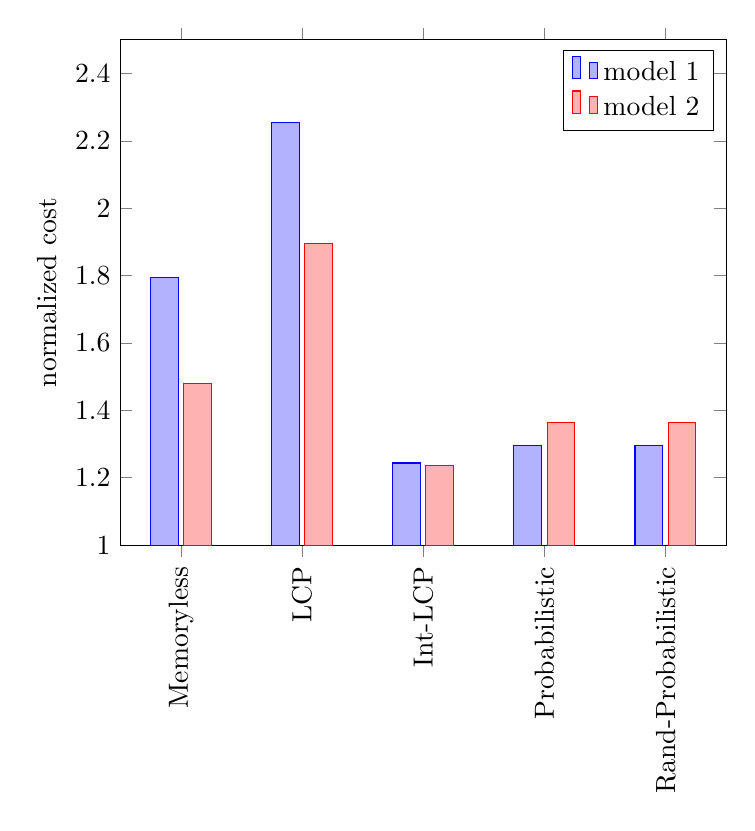
\begin{tikzpicture}

\begin{axis}[
ybar,
% bar width=0.5cm,
height=8cm,
% tick align=outside,
% tick pos=left,
% x grid style={white!69.0196078431373!black},
% xlabel={$OPT_s / OPT$},
xmin=-0.5, xmax=4.5,
xtick={0,1,2,3,4,5,6},
xticklabel style={rotate=90.0},
xticklabels={Memoryless,LCP,Int-LCP,Probabilistic,Rand-Probabilistic},
% xtick style={color=black},
% y grid style={white!69.0196078431373!black},
ylabel={normalized cost},
ymin=1, ymax=2.5,
% /pgf/number format/precision=5,
% ytick style={color=black}
]
\addplot
table {%
0 1.793108632
1 2.254697647
2 1.243801312
3 1.296624346
4 1.294611567
};
\addplot
table {%
0 1.479166878
1 1.895323607
2 1.235296539
3 1.363824754
4 1.363368466
};
\legend{model 1, model 2}
\end{axis}

\end{tikzpicture}
}
    \caption{LANL Mustang}
    \end{subfigure}
    \begin{subfigure}[b]{.48\linewidth}
    \resizebox{\textwidth}{!}{% This file was created by tikzplotlib v0.9.9.
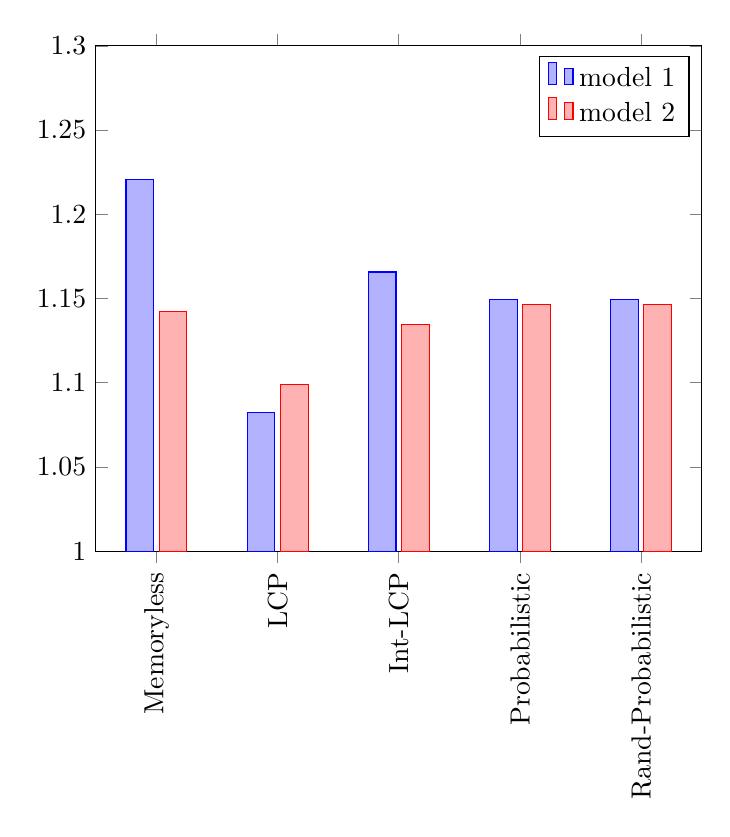
\begin{tikzpicture}

\begin{axis}[
ybar,
% bar width=0.5cm,
height=8cm,
% tick align=outside,
% tick pos=left,
% x grid style={white!69.0196078431373!black},
% xlabel={$OPT_s / OPT$},
xmin=-0.5, xmax=4.5,
xtick={0,1,2,3,4,5,6},
xticklabel style={rotate=90.0},
xticklabels={Memoryless,LCP,Int-LCP,Probabilistic,Rand-Probabilistic},
% xtick style={color=black},
% y grid style={white!69.0196078431373!black},
% ylabel={normalized cost},
ymin=1, ymax=1.3,
% /pgf/number format/precision=5,
% ytick style={color=black}
]
\addplot
table {%
0 1.220650656
1 1.082388905
2 1.165761722
3 1.149285464
4 1.149467892
};
\addplot
table {%
0 1.142369131
1 1.098736948
2 1.134416689
3 1.146620801
4 1.146662935
};
\legend{model 1, model 2}
\end{axis}

\end{tikzpicture}
}
    \caption{Alibaba}
    \end{subfigure}
    \caption{Normalized costs of uni-dimensional online algorithms. For the Facebook 2010 trace, the second model results in an optimal schedule constantly using all servers, explaining the disparate performance compared to the first model. Further, Probabilistic and Rand-Probabilistic perform very poorly in this setting and are therefore not shown for model 2. Generally, Probabilistic and Rand-Probabilistic achieve similar results. Interestingly, we observe that LCP outperforms Int-LCP when the potential cost reduction is small. In contrast, Int-LCP and the probabilistic algorithms outperform Memoryless and LCP significantly when the potential cost reduction is large. \Cref{fig:case_studies:ud:lcp_vs_int_lcp} compares the schedules obtained by LCP and Int-LCP in greater detail.}\label{fig:case_studies:ud:normalized_cost}
\end{figure}

\begin{figure}
    \begin{subfigure}[b]{.3425\linewidth}
    \resizebox{\textwidth}{!}{% This file was created by tikzplotlib v0.9.9.
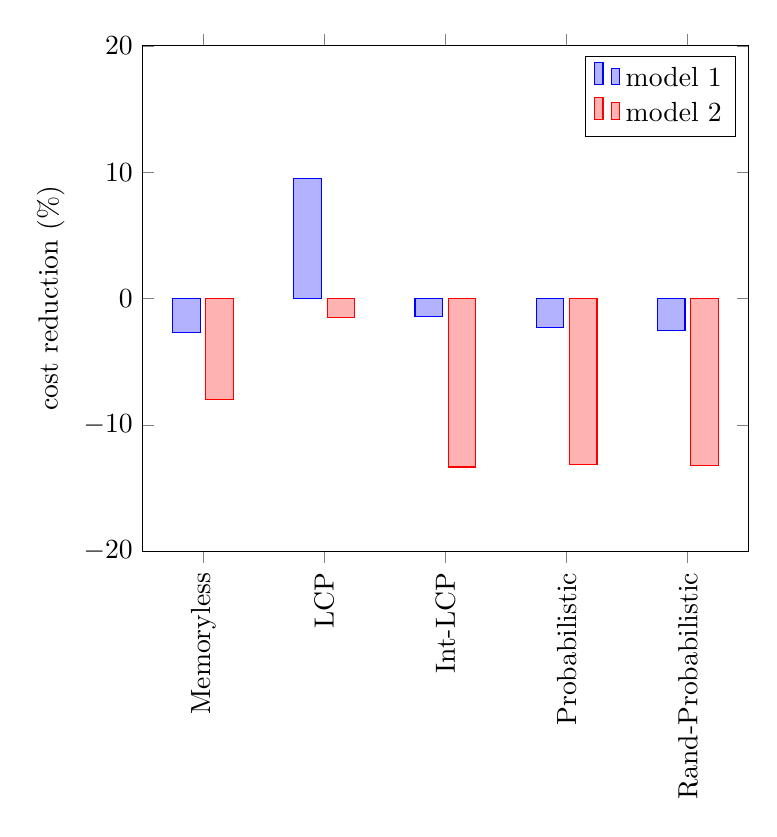
\begin{tikzpicture}

\begin{axis}[
ybar,
height=8cm,
% tick align=outside,
% tick pos=left,
% x grid style={white!69.0196078431373!black},
xmin=-0.5, xmax=4.5,
xtick={0,1,2,3,4,5,6},
xticklabel style={rotate=90.0},
xticklabels={Memoryless,LCP,Int-LCP,Probabilistic,Rand-Probabilistic},
% xtick style={color=black},
% y grid style={white!69.0196078431373!black},
ylabel={cost reduction (\%)},
ymin=-20, ymax=20,
/pgf/number format/precision=5,
% ytick style={color=black}
]
\addplot
table {%
0 -2.6773166
1 9.4800549
2 -1.43078
3 -2.3123229
4 -2.508807
};
\addplot
table {%
0 -8.0181426
1 -1.5303087
2 -13.3395591
3 -13.1603326
4 -13.2301154
};
\legend{model 1, model 2}
\end{axis}

\end{tikzpicture}
}
    \caption{Facebook 2009-0}
    \end{subfigure}
    \begin{subfigure}[b]{.32\linewidth}
    \resizebox{\textwidth}{!}{% This file was created by tikzplotlib v0.9.9.
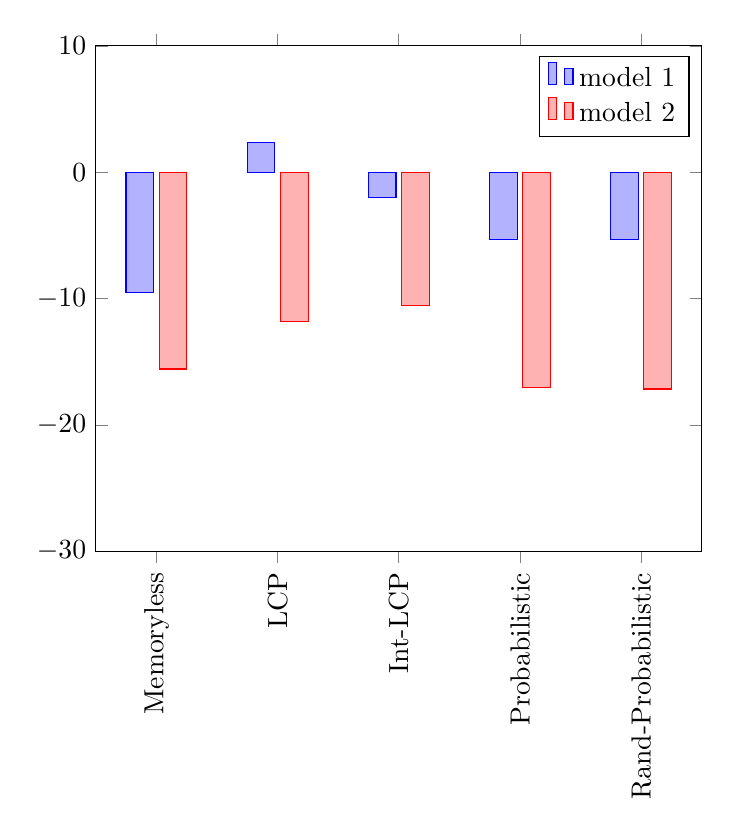
\begin{tikzpicture}

\begin{axis}[
ybar,
height=8cm,
% tick align=outside,
% tick pos=left,
% x grid style={white!69.0196078431373!black},
xmin=-0.5, xmax=4.5,
xtick={0,1,2,3,4,5,6},
xticklabel style={rotate=90.0},
xticklabels={Memoryless,LCP,Int-LCP,Probabilistic,Rand-Probabilistic},
% xtick style={color=black},
% y grid style={white!69.0196078431373!black},
% ylabel={cost reduction (\%)},
ymin=-30, ymax=10,
/pgf/number format/precision=5,
% ytick style={color=black}
]
\addplot
table {%
0 -9.5478387
1 2.3714279
2 -1.9899437
3 -5.3637334
4 -5.3637334
};
\addplot
table {%
0 -15.5769616
1 -11.7870895
2 -10.5657481
3 -17.0728106
4 -17.1640269
};
\legend{model 1, model 2}
\end{axis}

\end{tikzpicture}
}
    \caption{Facebook 2009-1}
    \end{subfigure}
    \begin{subfigure}[b]{.32\linewidth}
    \resizebox{\textwidth}{!}{% This file was created by tikzplotlib v0.9.9.
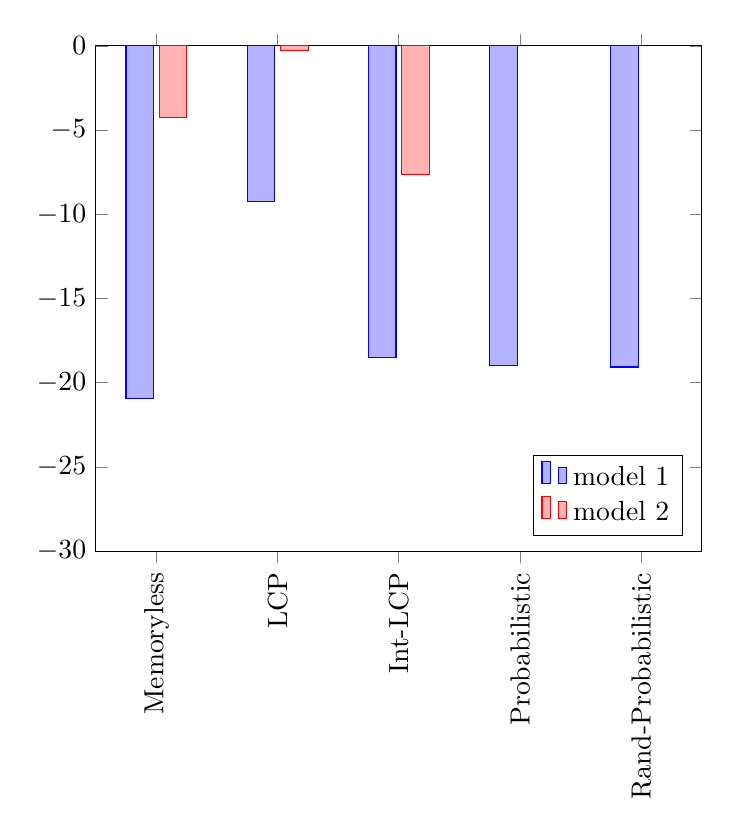
\begin{tikzpicture}

\begin{axis}[
legend pos=south east,
ybar,
height=8cm,
% tick align=outside,
% tick pos=left,
% x grid style={white!69.0196078431373!black},
xmin=-0.5, xmax=4.5,
xtick={0,1,2,3,4,5,6},
xticklabel style={rotate=90.0},
xticklabels={Memoryless,LCP,Int-LCP,Probabilistic,Rand-Probabilistic},
% xtick style={color=black},
% y grid style={white!69.0196078431373!black},
% ylabel={cost reduction (\%)},
ymin=-30, ymax=0,
/pgf/number format/precision=5,
% ytick style={color=black}
]
\addplot
table {%
0 -20.9191633
1 -9.233464
2 -18.4821319
3 -18.9948996
4 -19.0680432
};
\addplot
table {%
0 -4.2592762
1 -0.2849673
2 -7.620715
};
\legend{model 1, model 2}
\end{axis}

\end{tikzpicture}
}
    \caption{Facebook 2010}
    \end{subfigure}
    \par\bigskip
    \begin{subfigure}[b]{.50\linewidth}
    \resizebox{\textwidth}{!}{% This file was created by tikzplotlib v0.9.9.
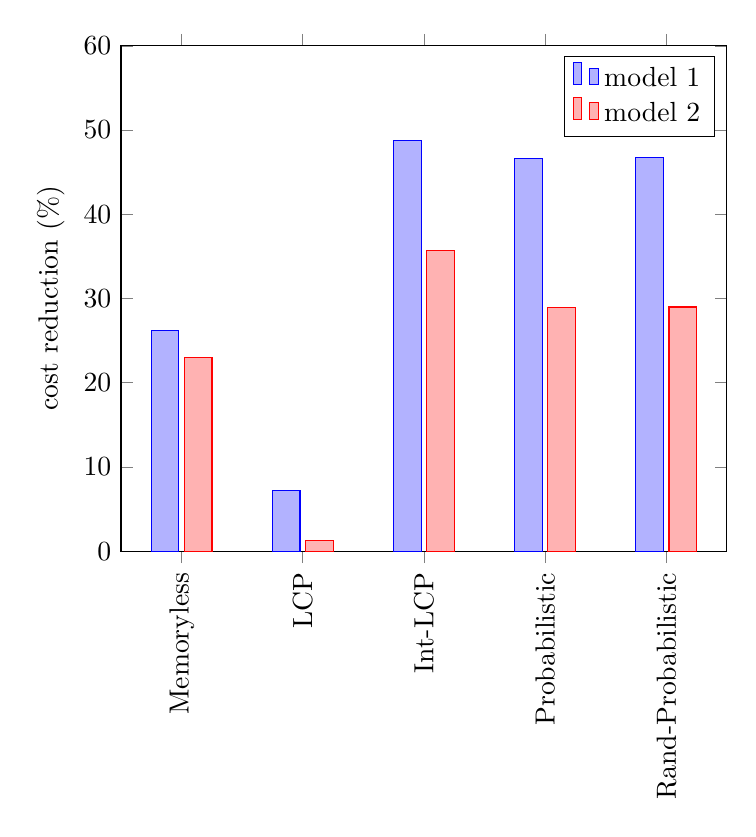
\begin{tikzpicture}

\begin{axis}[
ybar,
height=8cm,
% tick align=outside,
% tick pos=left,
% x grid style={white!69.0196078431373!black},
xmin=-0.5, xmax=4.5,
xtick={0,1,2,3,4,5,6},
xticklabel style={rotate=90.0},
xticklabels={Memoryless,LCP,Int-LCP,Probabilistic,Rand-Probabilistic},
% xtick style={color=black},
% y grid style={white!69.0196078431373!black},
ylabel={cost reduction (\%)},
ymin=0, ymax=60,
/pgf/number format/precision=5,
% ytick style={color=black}
]
\addplot
table {%
0 26.1928455
1 7.1931201
2 48.8031935
3 46.6289149
4 46.711764
};
\addplot
table {%
0 22.9634247
1 1.2895422
2 35.6644499
3 28.9705645
4 28.9943285
};
\legend{model 1, model 2}
\end{axis}

\end{tikzpicture}
}
    \caption{LANL Mustang}
    \end{subfigure}
    \begin{subfigure}[b]{.48\linewidth}
    \resizebox{\textwidth}{!}{% This file was created by tikzplotlib v0.9.9.
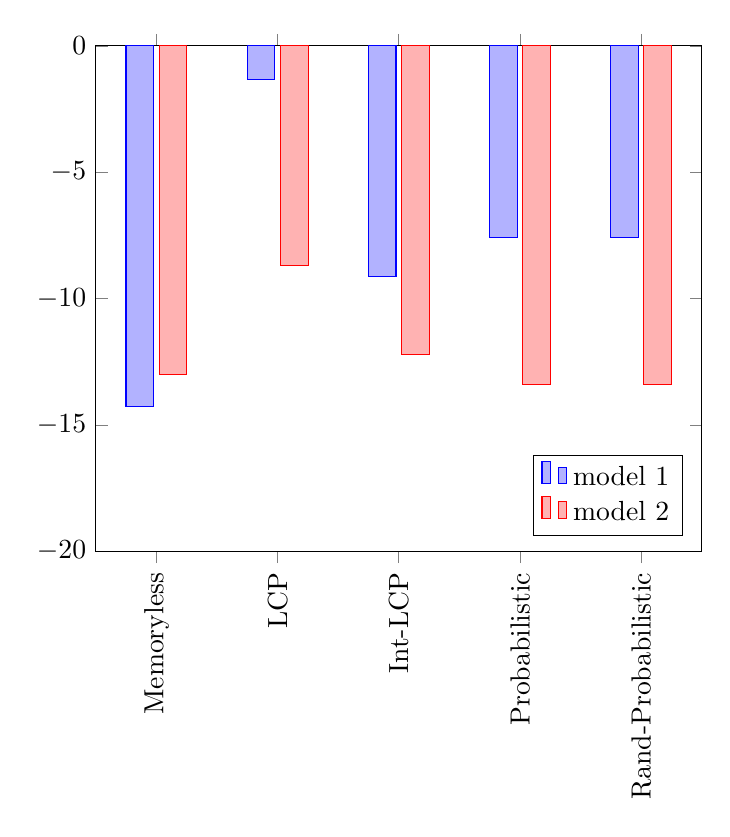
\begin{tikzpicture}

\begin{axis}[
legend pos=south east,
ybar,
height=8cm,
% tick align=outside,
% tick pos=left,
% x grid style={white!69.0196078431373!black},
xmin=-0.5, xmax=4.5,
xtick={0,1,2,3,4,5,6},
xticklabel style={rotate=90.0},
xticklabels={Memoryless,LCP,Int-LCP,Probabilistic,Rand-Probabilistic},
% xtick style={color=black},
% y grid style={white!69.0196078431373!black},
% ylabel={cost reduction (\%)},
ymin=-20, ymax=0,
/pgf/number format/precision=5,
% ytick style={color=black}
]
\addplot
table {%
0 -14.2617794
1 -1.3194739
2 -09.1237759
3 -07.5814783
4 -07.5985549
};
\addplot
table {%
0 -12.9927675
1 -8.6770686
2 -12.2061842
3 -13.413304
4 -13.4174715
};
\legend{model 1, model 2}
\end{axis}

\end{tikzpicture}
}
    \caption{Alibaba}
    \end{subfigure}
    \caption{Cost reduction of uni-dimensional online algorithms. For the Facebook 2010 trace, the second model results in an optimal schedule constantly using all servers, explaining the disparate performance compared to the first model. Further, Probabilistic and Rand-Probabilistic perform very poorly in this setting and are therefore not shown for model 2. Results are mainly determined by the normalized cost and the potential cost reduction (or static/dynamic ratio). We observe that the achieved cost reduction is dominated by the potential cost reduction (see \cref{fig:case_studies:ud:cost_reduction_vs_normalized_cost}).}\label{fig:case_studies:ud:cost_reduction}
\end{figure}

\begin{figure}
    \centering
    \pgfplotstableread{
X Y
-2.6773166 1.217963395
9.4800549 1.073752054
-1.43078 1.203176915
-2.3123229 1.213633822
-2.508807 1.215964525
-9.5478387 1.264233547
2.3714279 1.126679608
-1.9899437 1.177011887
-5.3637334 1.215947005
-5.3637334 1.215947005
-20.9191633 1.267149747
-9.233464 1.144691647
-18.4821319 1.241611332
-18.9948996 1.246984786
-19.0680432 1.24775128
26.1928455 1.793108632
7.1931201 2.254697647
48.8031935 1.243801312
46.6289149 1.296624346
46.711764 1.294611567
-14.2617794 1.220650656
-1.3194739 1.082388905
-09.1237759 1.165761722
-07.5814783 1.149285464
-07.5985549 1.149467892
}\a
\pgfplotstableread{
X Y
-8.0181426 1.157784554
-1.5303087 1.088245181
-13.3395591 1.214821767
-13.1603326 1.212900741
-13.2301154 1.213648703
-15.5769616 1.205891207
-11.7870895 1.166348954
-10.5657481 1.153605888
-17.0728106 1.221498393
-17.1640269 1.222450113
-4.2592762 1.042592762
-0.2849673 1.002849673
-7.620715 1.07620715
22.9634247 1.479166878
1.2895422 1.895323607
35.6644499 1.235296539
28.9705645 1.363824754
28.9943285 1.363368466
-12.9927675 1.142369131
-8.6770686 1.098736948
-12.2061842 1.134416689
-13.413304 1.146620801
-13.4174715 1.146662935
}\b

\begin{tikzpicture}
\begin{axis}[
legend pos=north east,
xlabel={cost reduction (\%)},
ylabel={normalized cost}]
\addplot [only marks, blue, mark = o] table {\a};
\addlegendentry{model 1}
\addplot [only marks, red, mark = o] table {\b};
\addlegendentry{model 2}
\addplot [thick, blue] table[
    y={create col/linear regression={y=Y}}
] % compute a linear regression from the input table
{\a};
\addplot [thick, red] table[
    y={create col/linear regression={y=Y}}
] % compute a linear regression from the input table
{\b};
\end{axis}
\end{tikzpicture}
    \caption{Weak positive correlation of achieved normalized cost and cost reduction. Intuitively, one would expect a strong negative correlation, i.e., the achieved cost reduction increases as the normalized cost approaches 1. Here, we find a positive correlation as the achieved cost reduction is dominated by the potential cost reduction (see \cref{fig:case_studies:ud:opt_vs_opts_against_mean_cost_reduction}).}\label{fig:case_studies:ud:cost_reduction_vs_normalized_cost}
\end{figure}

\paragraph{Normalized Cost} In the application of right-sizing data centers, we are interested in the cost associated with integral schedules. \Cref{fig:case_studies:ud:normalized_cost} shows the normalized cost of each algorithm. For fractional algorithms, we consider the cost of the associated integral schedule obtained by ceiling each configuration. Notably, LCP and Int-LCP perform differently depending on the trace and used model. We explore this behavior in \cref{fig:case_studies:ud:lcp_vs_int_lcp}.

\paragraph{Cost Reduction} \Cref{fig:case_studies:ud:cost_reduction} shows the achieved cost reduction. In general, we observe in \cref{fig:case_studies:ud:opt_vs_opts_against_normalized_cost}, \cref{fig:case_studies:ud:opt_vs_opts_against_mean_cost_reduction}, and \cref{fig:case_studies:ud:cost_reduction_vs_normalized_cost} that the achieved cost reduction is dominated by the potential cost reduction (which is mainly influenced by the PMR, see \cref{fig:case_studies:ud:opt_vs_opts:pmr}). When the potential cost reduction is small, algorithms with a smaller normalized cost in a particular setting, achieve a significantly higher cost reduction.

\begin{figure}
    \begin{subfigure}[b]{.5175\linewidth}
    \resizebox{\textwidth}{!}{% This file was created by tikzplotlib v0.9.9.
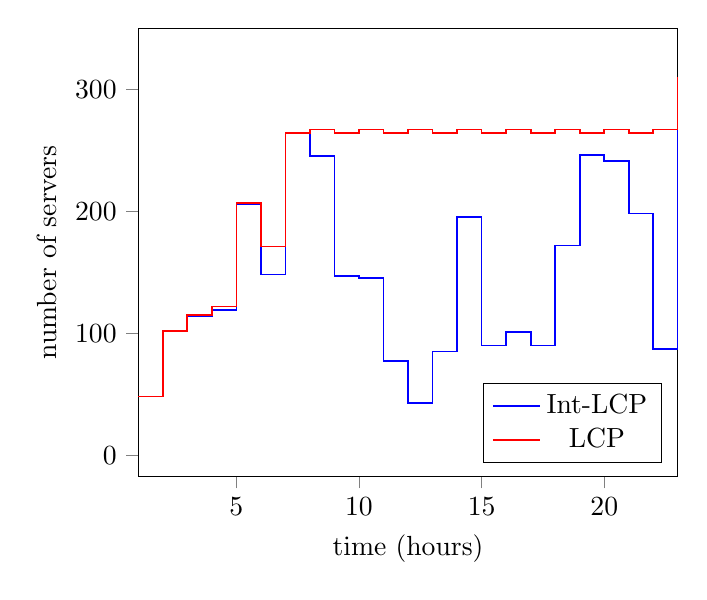
\begin{tikzpicture}

\begin{axis}[
legend pos=south east,
tick align=outside,
tick pos=left,
% x grid style={white!69.0196078431373!black},
xlabel={time (hours)},
xmin=1, xmax=23,
% xtick style={color=black},
% y grid style={white!69.0196078431373!black},
ylabel={number of servers},
ymin=-17.5, ymax=350,
% ytick style={color=black}
]
\addplot [semithick, blue, const plot mark left]
table {%
1 48
2 102
3 114
4 119
5 206
6 148
7 264
8 245
9 147
10 145
11 77
12 43
13 85
14 195
15 90
16 101
17 90
18 172
19 246
20 241
21 198
22 87
23 309
};
\addlegendentry{Int-LCP}
\addplot [semithick, red, const plot mark left]
table {%
1 48
2 102
3 115
4 122
5 207
6 171
7 264
8 267
9 264
10 267
11 264
12 267
13 264
14 267
15 264
16 267
17 264
18 267
19 264
20 267
21 264
22 267
23 310
};
\addlegendentry{LCP}
\end{axis}

\end{tikzpicture}
}
    \caption{Facebook 2009-0}
    \end{subfigure}
    \begin{subfigure}[b]{.4825\linewidth}
    \resizebox{\textwidth}{!}{% This file was created by tikzplotlib v0.9.9.
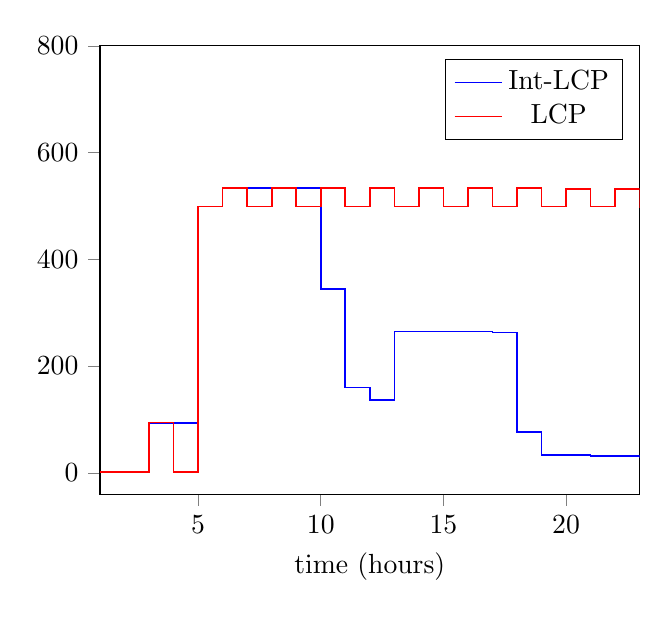
\begin{tikzpicture}

\begin{axis}[
legend pos=north east,
tick align=outside,
tick pos=left,
% x grid style={white!69.0196078431373!black},
xlabel={time (hours)},
xmin=1, xmax=23,
% xtick style={color=black},
% y grid style={white!69.0196078431373!black},
% ylabel={number of servers},
ymin=-40, ymax=800,
% ytick style={color=black}
]
\addplot [semithick, blue, const plot mark left]
table {%
1 1
2 1
3 93
4 93
5 499
6 533
7 533
8 533
9 533
10 344
11 160
12 136
13 265
14 265
15 265
16 265
17 263
18 76
19 33
20 33
21 32
22 31
23 30
24 30
};
\addlegendentry{Int-LCP}
\addplot [semithick, red, const plot mark left]
table {%
1 1
2 1
3 94
4 1
5 499
6 534
7 499
8 533
9 499
10 533
11 499
12 533
13 499
14 533
15 499
16 533
17 499
18 533
19 499
20 532
21 499
22 532
23 498
24 532
};
\addlegendentry{LCP}
\end{axis}

\end{tikzpicture}
}
    \caption{LANL Mustang}
    \end{subfigure}
    \caption{Comparison of the schedules obtained by LCP and Int-LCP under our first model. We observe that LCP is much ``stickier'' than Int-LCP, which is beneficial when the potential cost reduction is small (i.e., for the Facebook 2009-0 trace) but detrimental when the potential cost reduction is large (i.e., for the LANL Mustang trace). In our experiments, we observe that the memoryless algorithm tends to behave similarly to LCP (i.e., is more ``sticky''), whereas the probabilistic algorithms tend to behave similarly to Int-LCP (i.e., are less ``sticky'').}\label{fig:case_studies:ud:lcp_vs_int_lcp}
\end{figure}

\begin{figure}
    \begin{subfigure}[b]{.5175\linewidth}
    \resizebox{\textwidth}{!}{% This file was created by tikzplotlib v0.9.9.
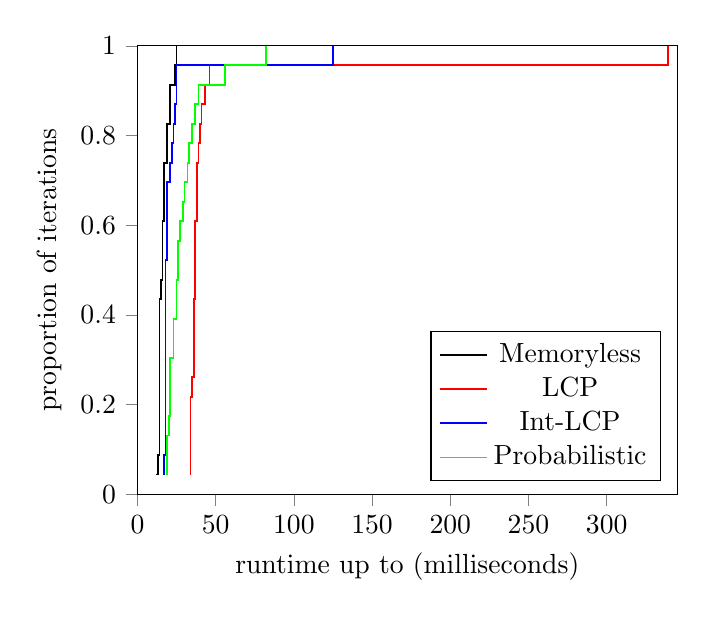
\begin{tikzpicture}

\definecolor{color0}{rgb}{0.12156862745098,0.466666666666667,0.705882352941177}

\begin{axis}[
legend pos=south east,
tick align=outside,
tick pos=left,
% x grid style={white!69.0196078431373!black},
xlabel={runtime up to (milliseconds)},
xmin=0, xmax=345,
% xtick style={color=black},
% y grid style={white!69.0196078431373!black},
ylabel={proportion of iterations},
ymin=0, ymax=1,
% ytick style={color=black}
]
\addplot [semithick, black, const plot mark left]
table {%
-inf 0
12 0.0434782608695652
13 0.0869565217391304
14 0.130434782608696
14 0.173913043478261
14 0.217391304347826
14 0.260869565217391
14 0.304347826086957
14 0.347826086956522
14 0.391304347826087
14 0.434782608695652
15 0.478260869565217
16 0.521739130434783
16 0.565217391304348
16 0.608695652173913
17 0.652173913043478
17 0.695652173913043
17 0.739130434782609
19 0.782608695652174
19 0.826086956521739
21 0.869565217391304
21 0.91304347826087
24 0.956521739130435
25 1
};
\addlegendentry{Memoryless}
\addplot [semithick, red, const plot mark left]
table {%
-inf 0
34 0.0434782608695652
34 0.0869565217391304
34 0.130434782608696
34 0.173913043478261
34 0.217391304347826
35 0.260869565217391
36 0.304347826086957
36 0.347826086956522
36 0.391304347826087
36 0.434782608695652
37 0.478260869565217
37 0.521739130434783
37 0.565217391304348
37 0.608695652173913
38 0.652173913043478
38 0.695652173913043
38 0.739130434782609
39 0.782608695652174
40 0.826086956521739
41 0.869565217391304
43 0.91304347826087
46 0.956521739130435
339 1
};
\addlegendentry{LCP}
\addplot [semithick, blue, const plot mark left]
table {%
-inf 0
17 0.0434782608695652
17 0.0869565217391304
18 0.130434782608696
18 0.173913043478261
18 0.217391304347826
18 0.260869565217391
18 0.304347826086957
18 0.347826086956522
18 0.391304347826087
18 0.434782608695652
18 0.478260869565217
18 0.521739130434783
19 0.565217391304348
19 0.608695652173913
19 0.652173913043478
19 0.695652173913043
21 0.739130434782609
22 0.782608695652174
23 0.826086956521739
24 0.869565217391304
25 0.91304347826087
25 0.956521739130435
125 1
};
\addlegendentry{Int-LCP}
\addplot [semithick, green, const plot mark left]
table {%
-inf 0
19 0.0434782608695652
19 0.0869565217391304
19 0.130434782608696
20 0.173913043478261
21 0.217391304347826
21 0.260869565217391
21 0.304347826086957
23 0.347826086956522
23 0.391304347826087
25 0.434782608695652
25 0.478260869565217
26 0.521739130434783
26 0.565217391304348
27 0.608695652173913
29 0.652173913043478
30 0.695652173913043
32 0.739130434782609
33 0.782608695652174
35 0.826086956521739
37 0.869565217391304
39 0.91304347826087
56 0.956521739130435
82 1
};
\addlegendentry{Probabilistic}
\end{axis}

\end{tikzpicture}}
    \end{subfigure}
    \begin{subfigure}[b]{.4825\linewidth}
    \resizebox{\textwidth}{!}{% This file was created by tikzplotlib v0.9.9.
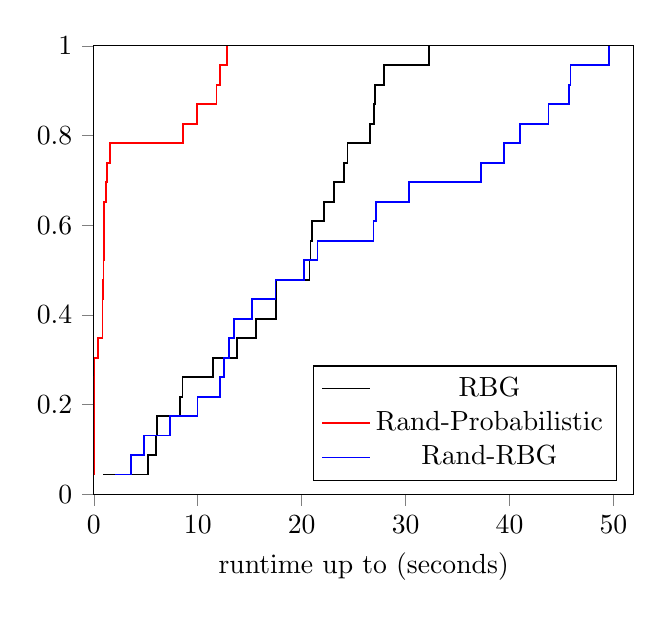
\begin{tikzpicture}

\definecolor{color0}{rgb}{0.12156862745098,0.466666666666667,0.705882352941177}

\begin{axis}[
legend pos=south east,
tick align=outside,
tick pos=left,
% x grid style={white!69.0196078431373!black},
xlabel={runtime up to (seconds)},
xmin=0, xmax=51.92685,
% xtick style={color=black},
% y grid style={white!69.0196078431373!black},
% ylabel={proportion of iterations},
ymin=0, ymax=1,
% ytick style={color=black}
]
\addplot [semithick, black, const plot mark left]
table {%
-inf 0
0.899 0.0434782608695652
5.188 0.0869565217391304
5.970 0.130434782608696
6.082 0.173913043478261
8.319 0.217391304347826
8.520 0.260869565217391
11.494 0.304347826086957
13.746 0.347826086956522
15.577 0.391304347826087
17.512 0.434782608695652
17.582 0.478260869565217
20.751 0.521739130434783
20.844 0.565217391304348
20.983 0.608695652173913
22.138 0.652173913043478
23.118 0.695652173913043
24.052 0.739130434782609
24.417 0.782608695652174
26.578 0.826086956521739
26.969 0.869565217391304
27.059 0.91304347826087
27.943 0.956521739130435
32.218 1
};
\addlegendentry{RBG}
\addplot [semithick, red, const plot mark left]
table {%
-inf 0
0.038 0.0434782608695652
0.040 0.0869565217391304
0.042 0.130434782608696
0.043 0.173913043478261
0.044 0.217391304347826
0.044 0.260869565217391
0.063 0.304347826086957
0.397 0.347826086956522
0.847 0.391304347826087
0.848 0.434782608695652
0.902 0.478260869565217
0.942 0.521739130434783
0.947 0.565217391304348
0.952 0.608695652173913
0.957 0.652173913043478
1.190 0.695652173913043
1.244 0.739130434782609
1.548 0.782608695652174
8.596 0.826086956521739
9.897 0.869565217391304
11.814 0.91304347826087
12.139 0.956521739130435
12.811 1
};
\addlegendentry{Rand-Probabilistic}
\addplot [semithick, blue, const plot mark left]
table {%
-inf 0
2.076 0.0434782608695652
3.585 0.0869565217391304
4.839 0.130434782608696
7.304 0.173913043478261
9.970 0.217391304347826
12.112 0.260869565217391
12.530 0.304347826086957
12.998 0.347826086956522
13.502 0.391304347826087
15.231 0.434782608695652
17.479 0.478260869565217
20.211 0.521739130434783
21.512 0.565217391304348
26.908 0.608695652173913
27.137 0.652173913043478
30.352 0.695652173913043
37.282 0.739130434782609
39.441 0.782608695652174
40.975 0.826086956521739
43.737 0.869565217391304
45.694 0.91304347826087
45.870 0.956521739130435
49.553 1
};
\addlegendentry{Rand-RBG}
\end{axis}

\end{tikzpicture}
}
    \end{subfigure}
    \caption{Runtimes of uni-dimensional online algorithms.}\label{fig:case_studies:ud:runtimes}
\end{figure}

\paragraph{Runtime} \cref{fig:case_studies:ud:runtimes} shows the distribution of runtimes (per iteration) of the online algorithms using the Facebook 2009-1 trace. The memoryless algorithm, LCP, and Int-LCP are very fast, even as the number of time slots increases. The runtime of Probabilistic and Rand-Probabilistic is slightly dependent on the used trace and model but generally good. However, when resulting schedules are thight around the upper bound of the decision space, as is the case for the Facebook 2010 trace under our second model, the probabilistic algorithms perform take multiple minutes per iteration. Rand-Probabilistic is significantly slower than Probabilistic as due to the relaxation the integrals need to be computed in a piecewise fashion. The runtime of RBG grows linearly with time and is shown in \cref{fig:case_studies:ud:runtimes} for the first four time slots.

\begin{figure}
    \centering
    % This file was created by tikzplotlib v0.9.9.
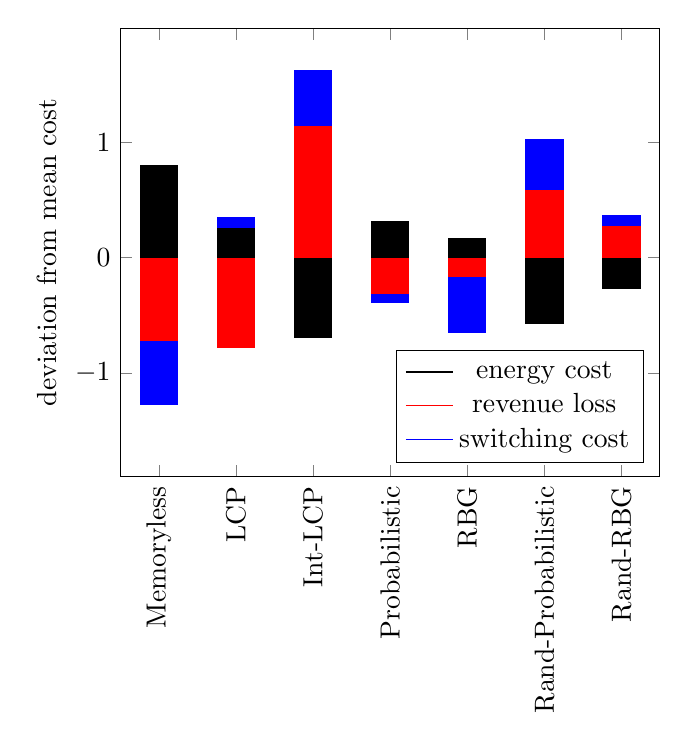
\begin{tikzpicture}

\begin{axis}[
% legend cell align={left},
% legend style={fill opacity=0.8, draw opacity=1, text opacity=1, draw=white!80!black},
legend pos=south east,
% tick align=outside,
% tick pos=left,
% x grid style={white!69.0196078431373!black},
xmin=-0.5, xmax=6.5,
% xtick style={color=black},
xtick={0,1,2,3,4,5,6},
xticklabel style={rotate=90.0},
xticklabels={Memoryless,LCP,Int-LCP,Probabilistic,RBG,Rand-Probabilistic,Rand-RBG},
% y grid style={white!69.0196078431373!black},
ylabel={deviation from mean cost},
ymin=-1.9, ymax=1.99,
% ytick style={color=black}
]
\draw[draw=none,fill=black] (axis cs:-0.25,0) rectangle (axis cs:0.25,0.807425489200161);
\addlegendimage{no markers,black}
\addlegendentry{energy cost}

\draw[draw=none,fill=black] (axis cs:0.75,0) rectangle (axis cs:1.25,0.259863816981542);
\draw[draw=none,fill=black] (axis cs:1.75,0) rectangle (axis cs:2.25,-0.700678355792212);
\draw[draw=none,fill=black] (axis cs:2.75,0) rectangle (axis cs:3.25,0.319075095160393);
\draw[draw=none,fill=black] (axis cs:3.75,0) rectangle (axis cs:4.25,0.168654808542322);
\draw[draw=none,fill=black] (axis cs:4.75,0) rectangle (axis cs:5.25,-0.580276790210896);
\draw[draw=none,fill=black] (axis cs:5.75,0) rectangle (axis cs:6.25,-0.274064063881251);
\draw[draw=none,fill=red] (axis cs:-0.25,0) rectangle (axis cs:0.25,-0.724683429714598);
\addlegendimage{no markers,red}
\addlegendentry{revenue loss}

\draw[draw=none,fill=red] (axis cs:0.75,0) rectangle (axis cs:1.25,-0.786649839499435);
\draw[draw=none,fill=red] (axis cs:1.75,0) rectangle (axis cs:2.25,1.14036434195245);
\draw[draw=none,fill=red] (axis cs:2.75,0) rectangle (axis cs:3.25,-0.318959604873333);
\draw[draw=none,fill=red] (axis cs:3.75,0) rectangle (axis cs:4.25,-0.168406286607572);
\draw[draw=none,fill=red] (axis cs:4.75,0) rectangle (axis cs:5.25,0.583295009974132);
\draw[draw=none,fill=red] (axis cs:5.75,0) rectangle (axis cs:6.25,0.275039808768246);
\draw[draw=none,fill=blue] (axis cs:-0.25,-0.724683429714598) rectangle (axis cs:0.25,-1.27941378667647);
\addlegendimage{no markers,blue}
\addlegendentry{switching cost}

\draw[draw=none,fill=blue] (axis cs:0.75,0.259863816981542) rectangle (axis cs:1.25,0.355127278784924);
\draw[draw=none,fill=blue] (axis cs:1.75,1.14036434195245) rectangle (axis cs:2.25,1.62741859052182);
\draw[draw=none,fill=blue] (axis cs:2.75,-0.318959604873333) rectangle (axis cs:3.25,-0.394731114222359);
\draw[draw=none,fill=blue] (axis cs:3.75,-0.168406286607572) rectangle (axis cs:4.25,-0.657894163636206);
\draw[draw=none,fill=blue] (axis cs:4.75,0.583295009974132) rectangle (axis cs:5.25,1.02713102645744);
\draw[draw=none,fill=blue] (axis cs:5.75,0.275039808768246) rectangle (axis cs:6.25,0.36887582525156);
\end{axis}

\end{tikzpicture}

    \caption{Cost profiles of uni-dimensional online algorithms. Note that integral algorithms seem to prefer revenue loss and switching costs over energy costs, whereas fractional algorithms prefer energy costs. However, this is likely because integral algorithms balance energy costs and revenue loss more accurately than the ceiled schedules of fractional algorithms.}\label{fig:case_studies:ud:costs}
\end{figure}

\paragraph{Cost Makeup} An interesting aspect of the (integral) schedules obtained by the online algorithms is the makeup of their associated costs to understand whether an algorithm systematically prefers some cost over another. We measure this preference of an algorithm as the normalized deviation, i.e., the cost of the algorithm minus the mean cost among all algorithms divided by the standard deviation. We then average the results between all traces. \Cref{fig:case_studies:ud:costs} shows the cost profiles for each algorithm. We observe that fractional algorithms prefer energy cost over revenue loss and switching cost, while integral algorithms prefer revenue loss and switching cost over energy cost. This is likely because fractional algorithms cannot balance energy cost and revenue loss optimally. When fractional schedules are ceiled, this results in an additional energy cost while reducing revenue loss. In absolute terms, the deviations make up less than 1\% of the overall costs of each type.

\paragraph{} We have seen that even in our conservative model, significant cost savings with respect to the optimal static provisioning in hindsight can be achieved in practical settings when the PMR is large enough or the normalized switching cost is less than the typical valley length. Due to the conservative estimates of our model, it is likely that in practice, much more drastic cost savings are possible. For example, when energy costs are higher, or the switching costs are on the order of operating a server in an idle state for one hour rather than four hours.

\section{Multi-Dimensional Algorithms}

Now, we turn to the discussed multi-dimensional algorithms. We begin by analyzing the simplified settings, SLO and SBLO, from \cref{section:online_algorithms:md:lazy_budgeting}. Then, we analyze the gradient-based methods from \cref{section:online_algorithms:md:descent_methods}.

\subsection{Smoothed Load Optimization}

Recall that for SLO, during a single time slot a server can process at most one job. Hence, we cannot use dynamic job durations to model the different runtimes of jobs on servers with two GPUs and servers with eight GPUs. Instead, we use a simplified model based on our second model, which is described in \cref{tab:simp_model}. Note that we disregard revenue loss and that we assume, servers operate at full utilization (if they are active). Overall, we obtain the operating costs $c = (243.720, 219.348)$ and switching costs $\beta = (487.440, 663.672)$.

\begin{table}
    \centering
    \begin{tabularx}{\textwidth}{>{\bfseries}l|X}
        cost & simplified model \\\hline
        operating cost & servers with eight GPUs have $0.9$ times the energy consumption (per processed job) as servers with two GPUs due to improved cooling efficiency \\
        switching cost & servers with eight GPUs have $1.3$ times the switching cost as servers with two GPUs due to an increased associated risk \\
    \caption{Simplified model used in our case studies of SLO and SBLO. The model parameters are based on our second model described in \cref{tab:model}.}
    \end{tabularx}
    \label{tab:simp_model}
\end{table}

The achieved normalized cost and cost reduction of lazy budgeting are shown in \cref{fig:case_studies:md:slo:normalized_cost} and \cref{fig:case_studies:md:slo:cost_reduction}, respectively. The dynamic offline optimal schedule primarily uses 8-GPU-servers and only uses 2-GPU-servers for short periods. The static offline optimal schedule uses 122 8-GPU-servers and no 2-GPU-servers as they have a larger operating cost, which would have to be paid throughout the entire day. The lazy budgeting algorithms primarily use 2-GPU-servers due to their lower switching cost and stick with 8-GPU-servers once they were powered up. \Cref{fig:case_studies:md:slo:det:schedule} and \cref{fig:case_studies:md:slo:rand:schedule} show the schedules obtained by the online algorithms in comparison to the offline optimal schedule. The runtime of the deterministic and randomized variants is shown in \cref{fig:case_studies:md:slo:runtimes}.

\begin{figure}
    \begin{subfigure}[b]{.5\linewidth}
    \resizebox{\textwidth}{!}{% This file was created by tikzplotlib v0.9.9.
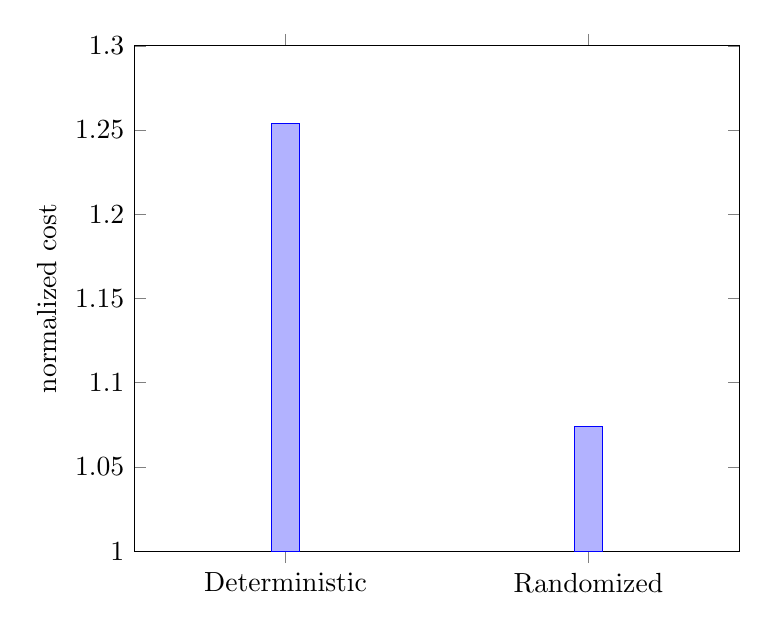
\begin{tikzpicture}

\begin{axis}[
ybar,
% bar width=0.5cm,
height=8cm,
% tick align=outside,
% tick pos=left,
% x grid style={white!69.0196078431373!black},
% xlabel={$OPT_s / OPT$},
xmin=-0.5, xmax=1.5,
xtick={0,1},
% xticklabel style={rotate=90.0},
xticklabels={Deterministic,Randomized},
% xtick style={color=black},
% y grid style={white!69.0196078431373!black},
ylabel={normalized cost},
ymin=1, ymax=1.3,
% /pgf/number format/precision=5,
% ytick style={color=black}
]
\addplot
table {%
0 1.254
1 1.074
};
\end{axis}

\end{tikzpicture}
}
    \caption{Normalized cost}\label{fig:case_studies:md:slo:normalized_cost}
    \end{subfigure}
    \begin{subfigure}[b]{.5\linewidth}
    \resizebox{\textwidth}{!}{\input{thesis/figures/slo_cost_reduction}}
    \caption{Cost reduction}\label{fig:case_studies:md:slo:cost_reduction}
    \end{subfigure}
    \caption{Performance of lazy budgeting (SLO) for the Microsoft Fiddle trace when compared against the offline optimum. The results of the randomized algorithm are based on five individual runs.}
\end{figure}

\begin{figure}
    \begin{subfigure}[b]{.3425\linewidth}
    \resizebox{\textwidth}{!}{\input{thesis/figures/slo_det_schedule}}
    \caption{SLO (deterministic)}\label{fig:case_studies:md:slo:det:schedule}
    \end{subfigure}
    \begin{subfigure}[b]{.32\linewidth}
    \resizebox{\textwidth}{!}{\input{thesis/figures/slo_rand_schedule}}
    \caption{SLO (randomized)}\label{fig:case_studies:md:slo:rand:schedule}
    \end{subfigure}
    \begin{subfigure}[b]{.32\linewidth}
    \resizebox{\textwidth}{!}{% This file was created by tikzplotlib v0.9.9.
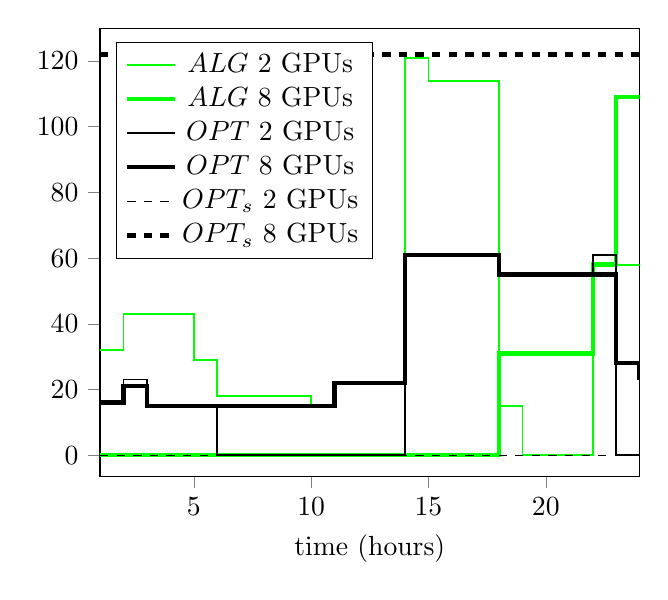
\begin{tikzpicture}

\begin{axis}[
legend pos=north west,
tick align=outside,
tick pos=left,
% x grid style={white!69.0196078431373!black},
xlabel={time (hours)},
xmin=1, xmax=24,
% xtick style={color=black},
% y grid style={white!69.0196078431373!black},
% ylabel={number of servers},
ymin=-6.5, ymax=130,
% ytick style={color=black}
]
\addplot [semithick, green, const plot mark left]
table {%
1 32
2 43
3 43
4 43
5 29
6 18
7 18
8 18
9 18
10 15
11 22
12 22
13 22
14 121
15 114
16 114
17 114
18 15
19 0
20 0
21 0
22 58
23 58
24 58
};
\addlegendentry{$ALG$ 2 GPUs}
\addplot [ultra thick, green, const plot mark left]
table {%
1 0
2 0
3 0
4 0
5 0
6 0
7 0
8 0
9 0
10 0
11 0
12 0
13 0
14 0
15 0
16 0
17 0
18 31
19 31
20 31
21 31
22 58
23 109
24 109
};
\addlegendentry{$ALG$ 8 GPUs}
\addplot [semithick, black, const plot mark left]
table {%
1 16
2 23
3 15
4 15
5 15
6 0
7 0
8 0
9 0
10 0
11 0
12 0
13 0
14 61
15 61
16 61
17 61
18 55
19 55
20 55
21 55
22 61
23 0
24 0
};
\addlegendentry{$OPT$ 2 GPUs}
\addplot [ultra thick, black, const plot mark left]
table {%
1 16
2 21
3 15
4 15
5 15
6 15
7 15
8 15
9 15
10 15
11 22
12 22
13 22
14 61
15 61
16 61
17 61
18 55
19 55
20 55
21 55
22 55
23 28
24 23
};
\addlegendentry{$OPT$ 8 GPUs}

\draw[dashed, color=black] (axis cs:\pgfkeysvalueof{/pgfplots/xmin},0) -- (axis cs:\pgfkeysvalueof{/pgfplots/xmax},0);
\addlegendimage{dashed, color=black}
\addlegendentry{$OPT_s$ 2 GPUs}
\draw[dashed, ultra thick, color=black] (axis cs:\pgfkeysvalueof{/pgfplots/xmin},122) -- (axis cs:\pgfkeysvalueof{/pgfplots/xmax},122);
\addlegendimage{dashed, ultra thick, color=black}
\addlegendentry{$OPT_s$ 8 GPUs}
\end{axis}

% \begin{axis}[
% axis y line*=right,
% axis x line=none,
% xmin=1, xmax=24,
% ymin=0, ymax=200,
% ylabel=load
% ]
% \addplot [semithick, red, const plot mark left]
% table {%
% 1 32
% 2 43
% 3 42
% 4 16
% 5 29
% 6 9
% 7 9
% 8 13
% 9 12
% 10 15
% 11 22
% 12 10
% 13 14
% 14 121
% 15 22
% 16 25
% 17 122
% 18 12
% 19 27
% 20 8
% 21 16
% 22 115
% 23 27
% 24 23
% };
% \end{axis}

\end{tikzpicture}
}
    \caption{SBLO ($\epsilon = 1/4$)}\label{fig:case_studies:md:sblo:schedule}
    \end{subfigure}
    \caption{Comparison of the schedules obtained by lazy budgeting for the Microsoft Fiddle trace and the offline optimum. For SLO, the deterministic algorithm is shown in blue and one result of the randomized algorithm is shown in red. The lazy budgeting algorithm for SBLO is shown in green. Note that the lazy budgeting algorithms prefer the 2-GPU-servers initially due to their low switching costs. For SLO, the randomized algorithm appears to be less ``sticky'' than the deterministic algorithm, resulting in a better normalized cost.}
\end{figure}

\begin{figure}
    \begin{subfigure}[b]{.5175\linewidth}
    \resizebox{\textwidth}{!}{% This file was created by tikzplotlib v0.9.9.
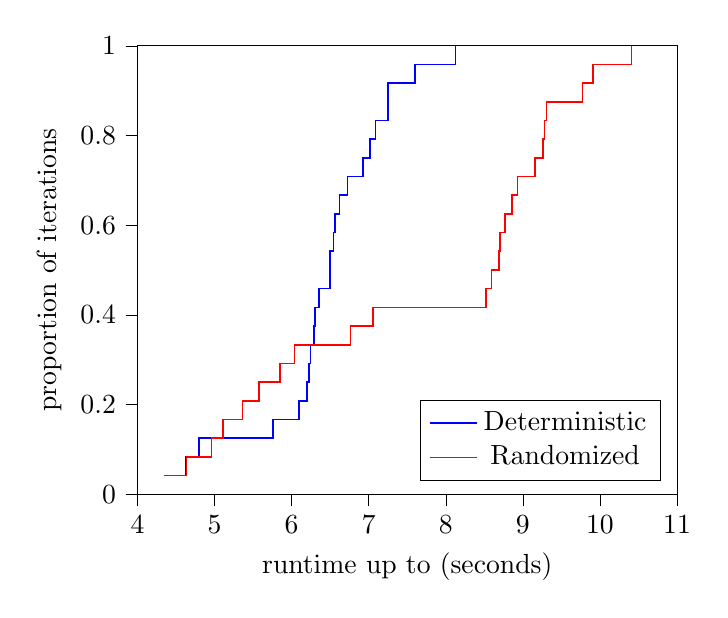
\begin{tikzpicture}

\definecolor{color0}{rgb}{0.12156862745098,0.466666666666667,0.705882352941177}

\begin{axis}[
legend pos=south east,
tick align=outside,
tick pos=left,
x grid style={white!69.0196078431373!black},
xlabel={runtime up to (seconds)},
xmin=4, xmax=11,
xtick style={color=black},
y grid style={white!69.0196078431373!black},
ylabel={proportion of iterations},
ymin=0, ymax=1,
ytick style={color=black}
]
\addplot [semithick, blue, const plot mark left]
table {%
-inf 0
4.565 0.0416666666666667
4.622 0.0833333333333333
4.802 0.125
5.756 0.166666666666667
6.093 0.208333333333333
6.199 0.25
6.224 0.291666666666667
6.245 0.333333333333333
6.291 0.375
6.301 0.416666666666667
6.354 0.458333333333333
6.496 0.5
6.498 0.541666666666667
6.541 0.583333333333333
6.561 0.625
6.621 0.666666666666667
6.724 0.708333333333333
6.924 0.75
7.019 0.791666666666667
7.088 0.833333333333333
7.248 0.875
7.251 0.916666666666667
7.597 0.958333333333333
8.125 1
};
\addlegendentry{Deterministic}
\addplot [semithick, red, const plot mark left]
table {%
-inf 0
4.339 0.0416666666666667
4.635 0.0833333333333333
4.960 0.125
5.111 0.166666666666667
5.362 0.208333333333333
5.573 0.25
5.852 0.291666666666667
6.036 0.333333333333333
6.764 0.375
7.052 0.416666666666667
8.518 0.458333333333333
8.593 0.5
8.688 0.541666666666667
8.699 0.583333333333333
8.770 0.625
8.860 0.666666666666667
8.932 0.708333333333333
9.157 0.75
9.264 0.791666666666667
9.279 0.833333333333333
9.308 0.875
9.773 0.916666666666667
9.906 0.958333333333333
10.410 1
};
\addlegendentry{Randomized}
\end{axis}

\end{tikzpicture}
}
    \caption{SLO}\label{fig:case_studies:md:slo:runtimes}
    \end{subfigure}
    \begin{subfigure}[b]{.4825\linewidth}
    \resizebox{\textwidth}{!}{% This file was created by tikzplotlib v0.9.9.
\begin{tikzpicture}

\definecolor{color0}{rgb}{0.12156862745098,0.466666666666667,0.705882352941177}

\begin{axis}[
legend pos=south east,
tick align=outside,
tick pos=left,
x grid style={white!69.0196078431373!black},
xlabel={runtime up to (seconds)},
xmin=25, xmax=50,
xtick style={color=black},
y grid style={white!69.0196078431373!black},
% ylabel={proportion of iterations},
ymin=0, ymax=1,
ytick style={color=black}
]
\addplot [semithick, blue, const plot mark left]
table {%
-inf 0
26.2298 0.0416666666666667
28.0695 0.0833333333333333
28.3796 0.125
28.8086 0.166666666666667
31.2105 0.208333333333333
31.6994 0.25
33.2586 0.291666666666667
33.9032 0.333333333333333
34.5655 0.375
34.8953 0.416666666666667
35.0067 0.458333333333333
35.5462 0.5
35.5884 0.541666666666667
35.8874 0.583333333333333
37.3382 0.625
37.6436 0.666666666666667
38.1931 0.708333333333333
38.4449 0.75
39.0436 0.791666666666667
39.1265 0.833333333333333
39.8516 0.875
41.2810 0.916666666666667
41.3132 0.958333333333333
48.2838 1
};
\end{axis}

\end{tikzpicture}
}
    \caption{SBLO}\label{fig:case_studies:md:sblo:runtimes}
    \end{subfigure}
    \caption{Runtime of lazy budgeting algorithms.}
\end{figure}

\subsection{Smoothed Balanced-Load Optimization}

For our analysis of SBLO, we use the same simplified model that we used in our analysis of SLO (see \cref{tab:simp_model}). In particular, we still assume that a server can at most process a single job during a time slot. The dynamic and static offline optimum are similar to those in our analysis of SLO. In particular, the static offline optimum still only uses 8-GPU-servers. \Cref{fig:case_studies:md:sblo:schedule} shows the schedule obtained by lazy budgeting ($\epsilon = 1/4$) in comparison with the offline optimal. Lazy budgeting achieves normalized costs 1.284 and a cost reduction of 11\%. The runtime of the algorithm is shown in \cref{fig:case_studies:md:sblo:runtimes}.

\subsection{Descent Methods}

We also evaluated the performance of P-OBD and D-OBD on the Microsoft Fiddle trace under our original models (see \cref{tab:model}). In our analysis we use the squared $\ell_2$ norm as the distance-generating function, i.e. $h(x) = \frac{1}{2} \norm{x}_2^2$, which is strongly convex and Lipschitz smooth in the $\ell_2$ norm. In our data center model, we use the $\ell_1$ norm to calculate switching costs, however, we observe that this approximation still achieves a good performance when compared against the dynamic offline optimum. The negative entropy $h(x) = \sum_{k=1}^d x_k \log_2 x_k$, which is commonly used as a distance-generating function for the $\ell_1$ norm cannot be used in the right-sizing data center setting as $\mathbf{0} \in \mathcal{X}$. \Cref{fig:case_studies:md:obd:normalized_cost} and \cref{fig:case_studies:md:obd:cost_reduction} show the achieved normalized cost and cost reduction. The resulting schedules under the first model are compared with the offline optimal in \cref{fig:case_studies:md:obd:schedule}. Remarkably, P-OBD and D-OBD obtain the exact same schedule under our second model. \Cref{fig:case_studies:md:obd:runtimes} visualizes the runtime of P-OBD and D-OBD under our first model.

\begin{figure}
    \begin{subfigure}[b]{.5\linewidth}
    \resizebox{\textwidth}{!}{% This file was created by tikzplotlib v0.9.9.
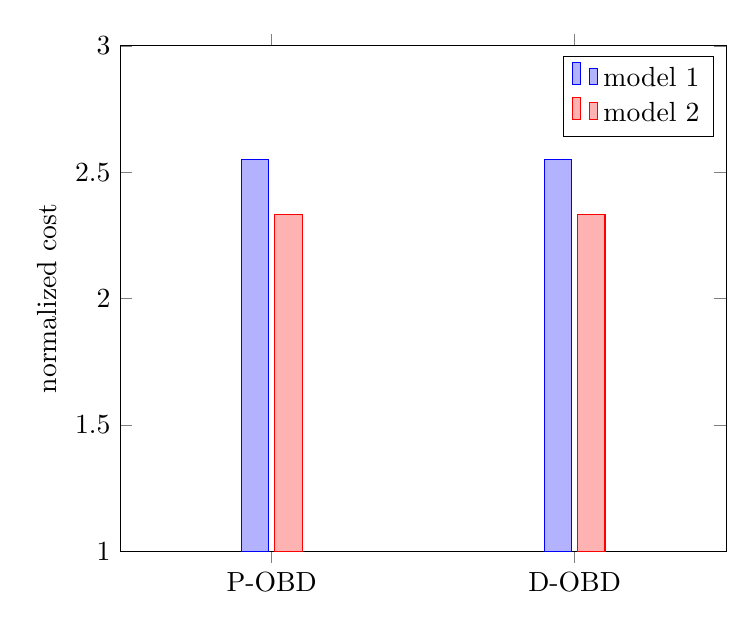
\begin{tikzpicture}

\begin{axis}[
ybar,
% bar width=0.5cm,
height=8cm,
% tick align=outside,
% tick pos=left,
% x grid style={white!69.0196078431373!black},
% xlabel={$OPT_s / OPT$},
xmin=-0.5, xmax=1.5,
xtick={0,1},
% xticklabel style={rotate=90.0},
xticklabels={P-OBD,D-OBD},
% xtick style={color=black},
% y grid style={white!69.0196078431373!black},
ylabel={normalized cost},
ymin=1, ymax=3,
% /pgf/number format/precision=5,
% ytick style={color=black}
]
\addplot
table {%
0 2.550
1 2.549
};
\addplot
table {%
0 2.334
1 2.334
};
\legend{model 1, model 2}
\end{axis}

\end{tikzpicture}
}
    \caption{Normalized cost}\label{fig:case_studies:md:obd:normalized_cost}
    \end{subfigure}
    \begin{subfigure}[b]{.5\linewidth}
    \resizebox{\textwidth}{!}{% This file was created by tikzplotlib v0.9.9.
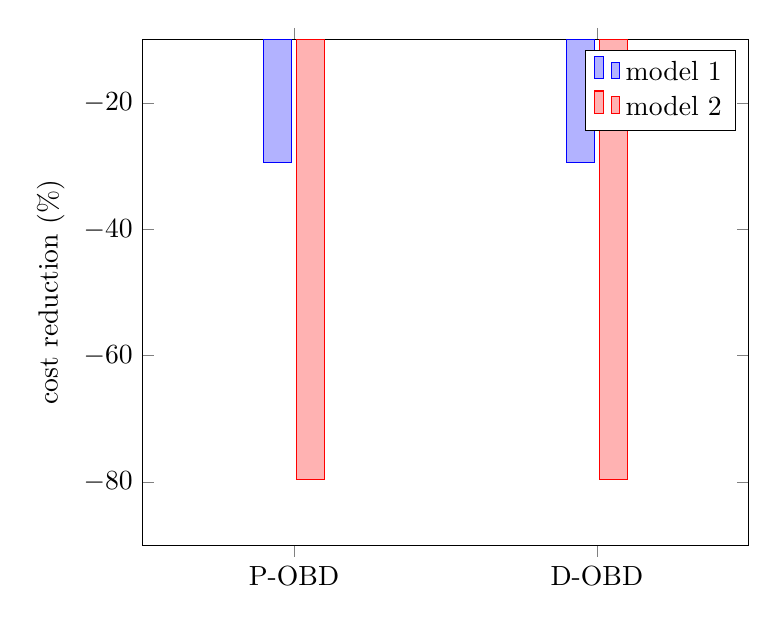
\begin{tikzpicture}

\begin{axis}[
ybar,
% bar width=0.5cm,
height=8cm,
% tick align=outside,
% tick pos=left,
% x grid style={white!69.0196078431373!black},
% xlabel={$OPT_s / OPT$},
xmin=-0.5, xmax=1.5,
xtick={0,1},
% xticklabel style={rotate=90.0},
xticklabels={P-OBD,D-OBD},
% xtick style={color=black},
% y grid style={white!69.0196078431373!black},
ylabel={cost reduction (\%)},
ymin=-90, ymax=-10,
% /pgf/number format/precision=5,
% ytick style={color=black}
]
\addplot
table {%
0 -29.485
1 -29.398
};
\addplot
table {%
0 -79.549
1 -79.549
};
\legend{model 1, model 2}
\end{axis}

\end{tikzpicture}
}
    \caption{Cost reduction}\label{fig:case_studies:md:obd:cost_reduction}
    \end{subfigure}
    \caption{Performance of P-OBD  ($\beta = 1/2$) and D-OBD  ($\eta = 1$) for the Microsoft Fiddle trace when compared against the offline optimum. $h(x) = \frac{1}{2} \norm{x}_2^2$ is used as the distance-generating function.}
\end{figure}

\begin{figure}
    \begin{subfigure}[b]{.5175\linewidth}
    \resizebox{\textwidth}{!}{% This file was created by tikzplotlib v0.9.9.
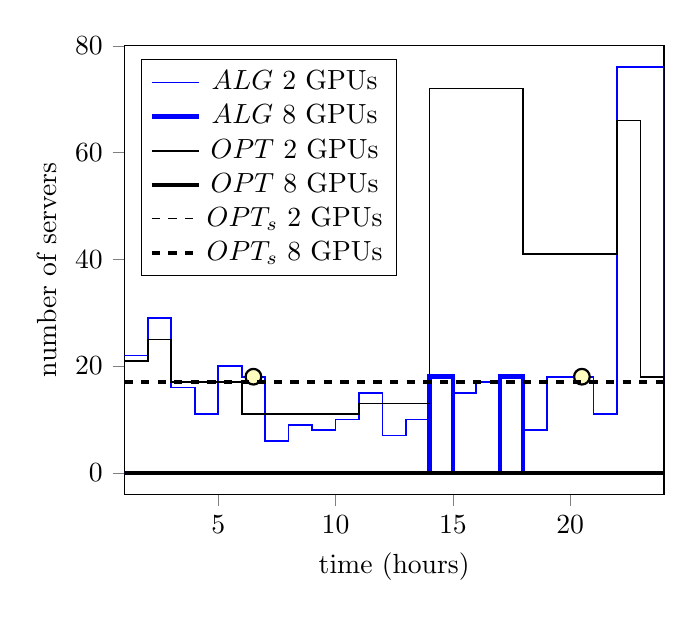
\begin{tikzpicture}

\begin{axis}[
legend pos=north west,
tick align=outside,
tick pos=left,
% x grid style={white!69.0196078431373!black},
xlabel={time (hours)},
xmin=1, xmax=24,
% xtick style={color=black},
% y grid style={white!69.0196078431373!black},
ylabel={number of servers},
ymin=-4, ymax=80,
% ytick style={color=black}
]
\addplot [semithick, blue, const plot mark left]
table {%
1 22
2 29
3 16
4 11
5 20
6 18
7 6
8 9
9 8
10 10
11 15
12 7
13 10
14 0
15 15
16 17
17 0
18 8
19 18
20 18
21 11
22 76
23 76
24 16
};
\addlegendentry{$ALG$ 2 GPUs}
\node (mark) [draw, fill=yellow!25, circle, minimum size = 5pt, inner sep=2pt, thick] 
      at (axis cs: 6.5, 18) {};
\node (mark) [draw, fill=yellow!25, circle, minimum size = 5pt, inner sep=2pt, thick] 
      at (axis cs: 20.5, 18) {};
\addplot [ultra thick, blue, const plot mark left]
table {%
1 0
2 0
3 0
4 0
5 0
6 0
7 0
8 0
9 0
10 0
11 0
12 0
13 0
14 18
15 0
16 0
17 18
18 0
19 0
20 0
21 0
22 0
23 0
24 0
};
\addlegendentry{$ALG$ 8 GPUs}
\addplot [semithick, black, const plot mark left]
table {%
1 21
2 25
3 17
4 17
5 17
6 11
7 11
8 11
9 11
10 11
11 13
12 13
13 13
14 72
15 72
16 72
17 72
18 41
19 41
20 41
21 41
22 66
23 18
24 15
};
\addlegendentry{$OPT$ 2 GPUs}
\addplot [ultra thick, black, const plot mark left]
table {%
1 0
2 0
3 0
4 0
5 0
6 0
7 0
8 0
9 0
10 0
11 0
12 0
13 0
14 0
15 0
16 0
17 0
18 0
19 0
20 0
21 0
22 0
23 0
24 0
};
\addlegendentry{$OPT$ 8 GPUs}

\draw[dashed, color=black] (axis cs:\pgfkeysvalueof{/pgfplots/xmin},0) -- (axis cs:\pgfkeysvalueof{/pgfplots/xmax},0);
\addlegendimage{dashed, color=black}
\addlegendentry{$OPT_s$ 2 GPUs}
\draw[dashed, ultra thick, color=black] (axis cs:\pgfkeysvalueof{/pgfplots/xmin},17) -- (axis cs:\pgfkeysvalueof{/pgfplots/xmax},17);
\addlegendimage{dashed, ultra thick, color=black}
\addlegendentry{$OPT_s$ 8 GPUs}
\end{axis}

% \begin{axis}[
% axis y line*=right,
% axis x line=none,
% xmin=1, xmax=24,
% ymin=0, ymax=200,
% ylabel=load
% ]
% \addplot [semithick, red, const plot mark left]
% table {%
% 1 32
% 2 43
% 3 42
% 4 16
% 5 29
% 6 9
% 7 9
% 8 13
% 9 12
% 10 15
% 11 22
% 12 10
% 13 14
% 14 121
% 15 22
% 16 25
% 17 122
% 18 12
% 19 27
% 20 8
% 21 16
% 22 115
% 23 27
% 24 23
% };
% \end{axis}

\end{tikzpicture}
}
    \caption{P-OBD}
    \end{subfigure}
    \begin{subfigure}[b]{.4825\linewidth}
    \resizebox{\textwidth}{!}{\input{thesis/figures/dobd_schedule}}
    \caption{D-OBD}
    \end{subfigure}
    \caption{Comparison of the schedules obtained by OBD for the Microsoft Fiddle trace under our first model and the offline optimum. P-OBD ($\beta = 1/2$) is shown in blue and D-OBD ($\eta = 1$) is shown in red. The two time slots during which P-OBD and D-OBD differ are marked in yellow ($t \in \{6, 20\}$). In both time slots, D-OBD is slightly less ``sticky'', resulting in a slightly better normalized cost. Also observe that under our first model, the dynamic offline optimum strictly prefers 2-GPU-servers over 8-GPU-servers In contrast, under our second model, 8-GPU-servers are slightly preferred by the dynamic offline optimum (see \cref{fig:microsoft:schedule}). $h(x) = \frac{1}{2} \norm{x}_2^2$ is used as the distance-generating function.}\label{fig:case_studies:md:obd:schedule}
\end{figure}

Although, OBD incurs an increased cost compared to the static offline optimal (the optimal static choice in hindsight) albeit by a factor less than 1, our very conservative model indicates that in practice, significant cost savings are possible.

\begin{figure}
    \centering
    % This file was created by tikzplotlib v0.9.9.
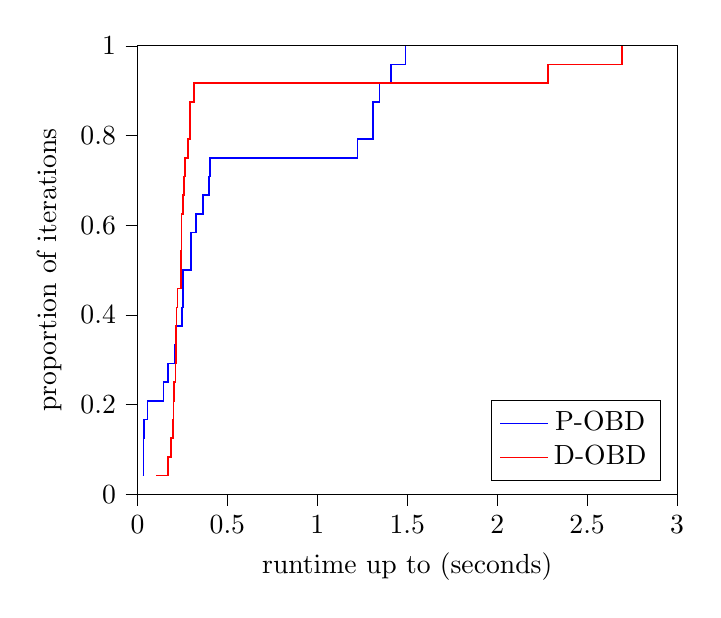
\begin{tikzpicture}

\begin{axis}[
legend pos=south east,
tick align=outside,
tick pos=left,
x grid style={white!69.0196078431373!black},
xlabel={runtime up to (seconds)},
xmin=0, xmax=3,
xtick style={color=black},
y grid style={white!69.0196078431373!black},
ylabel={proportion of iterations},
ymin=0, ymax=1,
ytick style={color=black}
]
\addplot [semithick, blue, const plot mark left]
table {%
-inf 0
0.029 0.0416666666666667
0.033 0.0833333333333333
0.034 0.125
0.038 0.166666666666667
0.055 0.208333333333333
0.144 0.25
0.170 0.291666666666667
0.209 0.333333333333333
0.212 0.375
0.246 0.416666666666667
0.254 0.458333333333333
0.255 0.5
0.297 0.541666666666667
0.297 0.583333333333333
0.326 0.625
0.363 0.666666666666667
0.396 0.708333333333333
0.404 0.75
1.223 0.791666666666667
1.308 0.833333333333333
1.309 0.875
1.345 0.916666666666667
1.409 0.958333333333333
1.490 1
};
\addlegendentry{P-OBD}
\addplot [semithick, red, const plot mark left]
table {%
-inf 0
0.105 0.0416666666666667
0.171 0.0833333333333333
0.188 0.125
0.197 0.166666666666667
0.201 0.208333333333333
0.204 0.25
0.212 0.291666666666667
0.216 0.333333333333333
0.216 0.375
0.218 0.416666666666667
0.222 0.458333333333333
0.242 0.5
0.243 0.541666666666667
0.244 0.583333333333333
0.244 0.625
0.252 0.666666666666667
0.259 0.708333333333333
0.265 0.75
0.280 0.791666666666667
0.292 0.833333333333333
0.293 0.875
0.313 0.916666666666667
2.283 0.958333333333333
2.695 1
};
\addlegendentry{D-OBD}
\end{axis}

\end{tikzpicture}

    \caption{Runtime of OBD algorithms.}\label{fig:case_studies:md:obd:runtimes}
\end{figure}

\section{Predictions}

In our analysis, we use the Alibaba trace under our second model to evaluate the effects of using predictions. We consider two different types of predictions: perfect predictions, and actual predictions that are obtained as described in \cref{section:online_algorithms:md:predictions:making_predictions}. The obtained predictions are based on the four preceding days of the Alibaba trace up until the second to last day. \Cref{fig:case_studies:predictions:prediction} visualizes the used prediction for the most common job type (i.e., short jobs). Note that in our analysis, we use the mean predicted load.

\begin{figure}
    \centering
    % This file was created by tikzplotlib v0.9.9.
\begin{tikzpicture}

\begin{axis}[
height=6cm,
width=\textwidth,
date coordinates in=x,
xlabel={day},
xmin=2018-01-01 15:54, xmax=2018-01-09 02:06,
xtick style={color=black},
xtick={2018-01-02 00:00,2018-01-03 00:00,2018-01-04 00:00,2018-01-05 00:00,2018-01-06 00:00,2018-01-07 00:00,2018-01-08 00:00,2018-01-09 00:00},
xticklabels={
  2,
  3,
  4,
  5,
  6,
  7,
  8,
  9
},
ylabel={load of short jobs},
ymin=0, ymax=205000,
]
\path [draw=black, fill=black, opacity=0.2]
(axis cs:2018-01-02 00:00:00+00:00,100098.696624773)
--(axis cs:2018-01-02 00:00:00+00:00,28288.5494373115)
--(axis cs:2018-01-02 01:00:00+00:00,37138.7334779417)
--(axis cs:2018-01-02 02:00:00+00:00,47680.1084426438)
--(axis cs:2018-01-02 03:00:00+00:00,63538.5324186298)
--(axis cs:2018-01-02 04:00:00+00:00,69628.2107901718)
--(axis cs:2018-01-02 05:00:00+00:00,62428.8761628568)
--(axis cs:2018-01-02 06:00:00+00:00,54208.5286179488)
--(axis cs:2018-01-02 07:00:00+00:00,46833.4699308402)
--(axis cs:2018-01-02 08:00:00+00:00,33026.7012040178)
--(axis cs:2018-01-02 09:00:00+00:00,25151.6151737295)
--(axis cs:2018-01-02 10:00:00+00:00,21088.0251495441)
--(axis cs:2018-01-02 11:00:00+00:00,17016.1299241989)
--(axis cs:2018-01-02 12:00:00+00:00,14501.184931781)
--(axis cs:2018-01-02 13:00:00+00:00,11529.998504521)
--(axis cs:2018-01-02 14:00:00+00:00,19025.1404347595)
--(axis cs:2018-01-02 15:00:00+00:00,8961.60319594767)
--(axis cs:2018-01-02 16:00:00+00:00,21448.251956248)
--(axis cs:2018-01-02 17:00:00+00:00,21782.8153633232)
--(axis cs:2018-01-02 18:00:00+00:00,31436.413168213)
--(axis cs:2018-01-02 19:00:00+00:00,37712.6162613149)
--(axis cs:2018-01-02 20:00:00+00:00,39983.0557354789)
--(axis cs:2018-01-02 21:00:00+00:00,33430.9276846751)
--(axis cs:2018-01-02 22:00:00+00:00,28254.2005086056)
--(axis cs:2018-01-02 23:00:00+00:00,23434.0123306569)
--(axis cs:2018-01-03 00:00:00+00:00,27855.7362822888)
--(axis cs:2018-01-03 01:00:00+00:00,38271.0633930584)
--(axis cs:2018-01-03 02:00:00+00:00,44902.7284545199)
--(axis cs:2018-01-03 03:00:00+00:00,59292.4268307121)
--(axis cs:2018-01-03 04:00:00+00:00,68572.4160847354)
--(axis cs:2018-01-03 05:00:00+00:00,63048.5466015148)
--(axis cs:2018-01-03 06:00:00+00:00,57075.5305401899)
--(axis cs:2018-01-03 07:00:00+00:00,48807.5967900616)
--(axis cs:2018-01-03 08:00:00+00:00,25807.094427619)
--(axis cs:2018-01-03 09:00:00+00:00,24450.2560800221)
--(axis cs:2018-01-03 10:00:00+00:00,24484.369408237)
--(axis cs:2018-01-03 11:00:00+00:00,18605.9684550062)
--(axis cs:2018-01-03 12:00:00+00:00,15657.6444362408)
--(axis cs:2018-01-03 13:00:00+00:00,16198.7277579188)
--(axis cs:2018-01-03 14:00:00+00:00,17507.5107772048)
--(axis cs:2018-01-03 15:00:00+00:00,15454.9693921289)
--(axis cs:2018-01-03 16:00:00+00:00,20889.7897899264)
--(axis cs:2018-01-03 17:00:00+00:00,28658.3784967043)
--(axis cs:2018-01-03 18:00:00+00:00,29940.2826066475)
--(axis cs:2018-01-03 19:00:00+00:00,35047.791488002)
--(axis cs:2018-01-03 20:00:00+00:00,36883.9080267522)
--(axis cs:2018-01-03 21:00:00+00:00,36069.7548192941)
--(axis cs:2018-01-03 22:00:00+00:00,25923.0051586477)
--(axis cs:2018-01-03 23:00:00+00:00,21059.1897620775)
--(axis cs:2018-01-04 00:00:00+00:00,26780.9058968163)
--(axis cs:2018-01-04 01:00:00+00:00,35902.2197065087)
--(axis cs:2018-01-04 02:00:00+00:00,50507.7049716134)
--(axis cs:2018-01-04 03:00:00+00:00,62423.4718977439)
--(axis cs:2018-01-04 04:00:00+00:00,69447.8855553915)
--(axis cs:2018-01-04 05:00:00+00:00,63347.6674782886)
--(axis cs:2018-01-04 06:00:00+00:00,59582.586652033)
--(axis cs:2018-01-04 07:00:00+00:00,47398.414212273)
--(axis cs:2018-01-04 08:00:00+00:00,27448.3529709349)
--(axis cs:2018-01-04 09:00:00+00:00,26525.0509343401)
--(axis cs:2018-01-04 10:00:00+00:00,22104.0523075594)
--(axis cs:2018-01-04 11:00:00+00:00,17281.6710962631)
--(axis cs:2018-01-04 12:00:00+00:00,18381.7755059042)
--(axis cs:2018-01-04 13:00:00+00:00,18266.9774682748)
--(axis cs:2018-01-04 14:00:00+00:00,12050.516342152)
--(axis cs:2018-01-04 15:00:00+00:00,13817.6157626535)
--(axis cs:2018-01-04 16:00:00+00:00,19417.6550925949)
--(axis cs:2018-01-04 17:00:00+00:00,21996.9172222188)
--(axis cs:2018-01-04 18:00:00+00:00,30581.6580755131)
--(axis cs:2018-01-04 19:00:00+00:00,37859.7236244808)
--(axis cs:2018-01-04 20:00:00+00:00,32716.3346696393)
--(axis cs:2018-01-04 21:00:00+00:00,34153.4582712529)
--(axis cs:2018-01-04 22:00:00+00:00,27747.7639793765)
--(axis cs:2018-01-04 23:00:00+00:00,22674.559311351)
--(axis cs:2018-01-05 00:00:00+00:00,23838.1340031656)
--(axis cs:2018-01-05 01:00:00+00:00,36882.5740346397)
--(axis cs:2018-01-05 02:00:00+00:00,49662.3091365488)
--(axis cs:2018-01-05 03:00:00+00:00,60936.0282518601)
--(axis cs:2018-01-05 04:00:00+00:00,71466.1188717826)
--(axis cs:2018-01-05 05:00:00+00:00,67350.5446137087)
--(axis cs:2018-01-05 06:00:00+00:00,57012.9766763558)
--(axis cs:2018-01-05 07:00:00+00:00,44275.7758893904)
--(axis cs:2018-01-05 08:00:00+00:00,29423.7349939941)
--(axis cs:2018-01-05 09:00:00+00:00,23328.6031012108)
--(axis cs:2018-01-05 10:00:00+00:00,19268.5344742425)
--(axis cs:2018-01-05 11:00:00+00:00,13367.5078259395)
--(axis cs:2018-01-05 12:00:00+00:00,14216.189406124)
--(axis cs:2018-01-05 13:00:00+00:00,17872.3107114167)
--(axis cs:2018-01-05 14:00:00+00:00,13991.6956652202)
--(axis cs:2018-01-05 15:00:00+00:00,16617.3958805225)
--(axis cs:2018-01-05 16:00:00+00:00,19766.9544734047)
--(axis cs:2018-01-05 17:00:00+00:00,28840.4668123843)
--(axis cs:2018-01-05 18:00:00+00:00,35148.804167733)
--(axis cs:2018-01-05 19:00:00+00:00,33416.9087639768)
--(axis cs:2018-01-05 20:00:00+00:00,37219.5488658414)
--(axis cs:2018-01-05 21:00:00+00:00,31838.3439341474)
--(axis cs:2018-01-05 22:00:00+00:00,30040.8277719143)
--(axis cs:2018-01-05 23:00:00+00:00,22163.2276014059)
--(axis cs:2018-01-06 00:00:00+00:00,26125.4464910477)
--(axis cs:2018-01-06 01:00:00+00:00,37773.1355100019)
--(axis cs:2018-01-06 02:00:00+00:00,50583.8693138311)
--(axis cs:2018-01-06 03:00:00+00:00,60154.3237049639)
--(axis cs:2018-01-06 04:00:00+00:00,69467.4449092172)
--(axis cs:2018-01-06 05:00:00+00:00,65770.3370393846)
--(axis cs:2018-01-06 06:00:00+00:00,55942.1305030647)
--(axis cs:2018-01-06 07:00:00+00:00,41797.9052318869)
--(axis cs:2018-01-06 08:00:00+00:00,27494.2624192075)
--(axis cs:2018-01-06 09:00:00+00:00,24682.3113639605)
--(axis cs:2018-01-06 10:00:00+00:00,22055.462486761)
--(axis cs:2018-01-06 11:00:00+00:00,12339.6647832355)
--(axis cs:2018-01-06 12:00:00+00:00,15223.5936930151)
--(axis cs:2018-01-06 13:00:00+00:00,14129.3834413131)
--(axis cs:2018-01-06 14:00:00+00:00,15398.1980007012)
--(axis cs:2018-01-06 15:00:00+00:00,20384.7572834536)
--(axis cs:2018-01-06 16:00:00+00:00,17948.3544981102)
--(axis cs:2018-01-06 17:00:00+00:00,27504.1556195579)
--(axis cs:2018-01-06 18:00:00+00:00,30849.6881543022)
--(axis cs:2018-01-06 19:00:00+00:00,33255.9399800159)
--(axis cs:2018-01-06 20:00:00+00:00,34668.9678931554)
--(axis cs:2018-01-06 21:00:00+00:00,33400.4728320907)
--(axis cs:2018-01-06 22:00:00+00:00,27697.6450379186)
--(axis cs:2018-01-06 23:00:00+00:00,20479.5388640444)
--(axis cs:2018-01-07 00:00:00+00:00,25393.5539136519)
--(axis cs:2018-01-07 01:00:00+00:00,36892.2827677412)
--(axis cs:2018-01-07 02:00:00+00:00,46389.4277248442)
--(axis cs:2018-01-07 03:00:00+00:00,61043.157415353)
--(axis cs:2018-01-07 04:00:00+00:00,64127.0388093701)
--(axis cs:2018-01-07 05:00:00+00:00,67365.3172651187)
--(axis cs:2018-01-07 06:00:00+00:00,56365.0672384231)
--(axis cs:2018-01-07 07:00:00+00:00,45618.7576312223)
--(axis cs:2018-01-07 08:00:00+00:00,37793.7838222988)
--(axis cs:2018-01-07 09:00:00+00:00,22830.9291765626)
--(axis cs:2018-01-07 10:00:00+00:00,19262.8667569174)
--(axis cs:2018-01-07 11:00:00+00:00,8629.10756986361)
--(axis cs:2018-01-07 12:00:00+00:00,15827.1074586404)
--(axis cs:2018-01-07 13:00:00+00:00,17202.6315084655)
--(axis cs:2018-01-07 14:00:00+00:00,16398.4122361792)
--(axis cs:2018-01-07 15:00:00+00:00,18548.3876754588)
--(axis cs:2018-01-07 16:00:00+00:00,15708.286876679)
--(axis cs:2018-01-07 17:00:00+00:00,27192.8408531418)
--(axis cs:2018-01-07 18:00:00+00:00,37129.1968090024)
--(axis cs:2018-01-07 19:00:00+00:00,36929.3539193636)
--(axis cs:2018-01-07 20:00:00+00:00,32622.7684089465)
--(axis cs:2018-01-07 21:00:00+00:00,33852.8120964986)
--(axis cs:2018-01-07 22:00:00+00:00,25629.3309198523)
--(axis cs:2018-01-07 23:00:00+00:00,23322.324807958)
--(axis cs:2018-01-08 00:00:00+00:00,22287.7174598704)
--(axis cs:2018-01-08 01:00:00+00:00,36529.6015052096)
--(axis cs:2018-01-08 02:00:00+00:00,54123.3887986232)
--(axis cs:2018-01-08 03:00:00+00:00,59785.3836388751)
--(axis cs:2018-01-08 04:00:00+00:00,68510.4178675914)
--(axis cs:2018-01-08 05:00:00+00:00,64527.60738026)
--(axis cs:2018-01-08 06:00:00+00:00,54937.6684090287)
--(axis cs:2018-01-08 07:00:00+00:00,46190.78485245)
--(axis cs:2018-01-08 08:00:00+00:00,31321.3608087154)
--(axis cs:2018-01-08 09:00:00+00:00,25725.6606826978)
--(axis cs:2018-01-08 10:00:00+00:00,20819.0527698839)
--(axis cs:2018-01-08 11:00:00+00:00,16447.9967085571)
--(axis cs:2018-01-08 12:00:00+00:00,17979.5904729499)
--(axis cs:2018-01-08 13:00:00+00:00,13947.5177469049)
--(axis cs:2018-01-08 14:00:00+00:00,18413.4869130723)
--(axis cs:2018-01-08 15:00:00+00:00,20240.129248887)
--(axis cs:2018-01-08 16:00:00+00:00,24810.1433065698)
--(axis cs:2018-01-08 17:00:00+00:00,21629.8628679309)
--(axis cs:2018-01-08 18:00:00+00:00,35421.351285177)
--(axis cs:2018-01-08 18:00:00+00:00,116305.703432731)
--(axis cs:2018-01-08 18:00:00+00:00,116305.703432731)
--(axis cs:2018-01-08 17:00:00+00:00,103589.247950974)
--(axis cs:2018-01-08 16:00:00+00:00,99580.6499476631)
--(axis cs:2018-01-08 15:00:00+00:00,96227.0177834567)
--(axis cs:2018-01-08 14:00:00+00:00,88112.2582938287)
--(axis cs:2018-01-08 13:00:00+00:00,87859.2975552475)
--(axis cs:2018-01-08 12:00:00+00:00,91550.4992276826)
--(axis cs:2018-01-08 11:00:00+00:00,92410.8146648707)
--(axis cs:2018-01-08 10:00:00+00:00,98503.8388203821)
--(axis cs:2018-01-08 09:00:00+00:00,97685.1849645065)
--(axis cs:2018-01-08 08:00:00+00:00,108112.139214545)
--(axis cs:2018-01-08 07:00:00+00:00,121643.751488121)
--(axis cs:2018-01-08 06:00:00+00:00,135264.546469844)
--(axis cs:2018-01-08 05:00:00+00:00,142072.194261612)
--(axis cs:2018-01-08 04:00:00+00:00,143208.641908423)
--(axis cs:2018-01-08 03:00:00+00:00,140871.495904598)
--(axis cs:2018-01-08 02:00:00+00:00,125602.505212183)
--(axis cs:2018-01-08 01:00:00+00:00,110712.251248938)
--(axis cs:2018-01-08 00:00:00+00:00,104934.932377308)
--(axis cs:2018-01-07 23:00:00+00:00,100310.216898447)
--(axis cs:2018-01-07 22:00:00+00:00,101624.427806836)
--(axis cs:2018-01-07 21:00:00+00:00,106174.444848886)
--(axis cs:2018-01-07 20:00:00+00:00,112122.630890364)
--(axis cs:2018-01-07 19:00:00+00:00,113796.989742922)
--(axis cs:2018-01-07 18:00:00+00:00,113626.276534999)
--(axis cs:2018-01-07 17:00:00+00:00,102089.451528019)
--(axis cs:2018-01-07 16:00:00+00:00,97666.196521732)
--(axis cs:2018-01-07 15:00:00+00:00,94064.0069188067)
--(axis cs:2018-01-07 14:00:00+00:00,89065.5551225934)
--(axis cs:2018-01-07 13:00:00+00:00,87336.657203696)
--(axis cs:2018-01-07 12:00:00+00:00,92478.4954525417)
--(axis cs:2018-01-07 11:00:00+00:00,92212.4158062934)
--(axis cs:2018-01-07 10:00:00+00:00,94859.6755574438)
--(axis cs:2018-01-07 09:00:00+00:00,97652.8356964389)
--(axis cs:2018-01-07 08:00:00+00:00,112290.10283372)
--(axis cs:2018-01-07 07:00:00+00:00,122014.302825006)
--(axis cs:2018-01-07 06:00:00+00:00,132511.892832446)
--(axis cs:2018-01-07 05:00:00+00:00,141246.386362709)
--(axis cs:2018-01-07 04:00:00+00:00,141961.007355637)
--(axis cs:2018-01-07 03:00:00+00:00,138429.674652609)
--(axis cs:2018-01-07 02:00:00+00:00,127013.830123646)
--(axis cs:2018-01-07 01:00:00+00:00,114662.650417302)
--(axis cs:2018-01-07 00:00:00+00:00,105278.978242448)
--(axis cs:2018-01-06 23:00:00+00:00,103170.597222355)
--(axis cs:2018-01-06 22:00:00+00:00,102580.6170794)
--(axis cs:2018-01-06 21:00:00+00:00,107852.478472186)
--(axis cs:2018-01-06 20:00:00+00:00,114085.727646972)
--(axis cs:2018-01-06 19:00:00+00:00,111956.933794231)
--(axis cs:2018-01-06 18:00:00+00:00,108882.021400531)
--(axis cs:2018-01-06 17:00:00+00:00,99917.7292622046)
--(axis cs:2018-01-06 16:00:00+00:00,96361.2807685625)
--(axis cs:2018-01-06 15:00:00+00:00,98225.9159212145)
--(axis cs:2018-01-06 14:00:00+00:00,88131.0883518406)
--(axis cs:2018-01-06 13:00:00+00:00,91382.558641352)
--(axis cs:2018-01-06 12:00:00+00:00,90357.2373213856)
--(axis cs:2018-01-06 11:00:00+00:00,93281.9826117533)
--(axis cs:2018-01-06 10:00:00+00:00,93805.3380345052)
--(axis cs:2018-01-06 09:00:00+00:00,99370.4698208578)
--(axis cs:2018-01-06 08:00:00+00:00,109455.812670362)
--(axis cs:2018-01-06 07:00:00+00:00,119682.529935301)
--(axis cs:2018-01-06 06:00:00+00:00,132890.035779861)
--(axis cs:2018-01-06 05:00:00+00:00,143339.260271051)
--(axis cs:2018-01-06 04:00:00+00:00,145519.275290207)
--(axis cs:2018-01-06 03:00:00+00:00,137869.41430717)
--(axis cs:2018-01-06 02:00:00+00:00,127280.047840281)
--(axis cs:2018-01-06 01:00:00+00:00,113265.636884808)
--(axis cs:2018-01-06 00:00:00+00:00,101759.123615318)
--(axis cs:2018-01-05 23:00:00+00:00,98386.2967889798)
--(axis cs:2018-01-05 22:00:00+00:00,102058.53604084)
--(axis cs:2018-01-05 21:00:00+00:00,107770.459242455)
--(axis cs:2018-01-05 20:00:00+00:00,113791.560599757)
--(axis cs:2018-01-05 19:00:00+00:00,111368.375350588)
--(axis cs:2018-01-05 18:00:00+00:00,111331.021460867)
--(axis cs:2018-01-05 17:00:00+00:00,104012.64233064)
--(axis cs:2018-01-05 16:00:00+00:00,100296.2171639)
--(axis cs:2018-01-05 15:00:00+00:00,90327.4276103283)
--(axis cs:2018-01-05 14:00:00+00:00,89964.5956644114)
--(axis cs:2018-01-05 13:00:00+00:00,86222.4463843374)
--(axis cs:2018-01-05 12:00:00+00:00,96159.5510036112)
--(axis cs:2018-01-05 11:00:00+00:00,92636.9325210587)
--(axis cs:2018-01-05 10:00:00+00:00,96896.8247438989)
--(axis cs:2018-01-05 09:00:00+00:00,98473.2170287393)
--(axis cs:2018-01-05 08:00:00+00:00,108028.963837113)
--(axis cs:2018-01-05 07:00:00+00:00,121240.489262855)
--(axis cs:2018-01-05 06:00:00+00:00,138985.058219831)
--(axis cs:2018-01-05 05:00:00+00:00,145113.849252422)
--(axis cs:2018-01-05 04:00:00+00:00,145100.910643194)
--(axis cs:2018-01-05 03:00:00+00:00,140649.884944644)
--(axis cs:2018-01-05 02:00:00+00:00,131538.686380006)
--(axis cs:2018-01-05 01:00:00+00:00,106754.93170765)
--(axis cs:2018-01-05 00:00:00+00:00,102716.925674879)
--(axis cs:2018-01-04 23:00:00+00:00,101596.326997732)
--(axis cs:2018-01-04 22:00:00+00:00,103206.580050618)
--(axis cs:2018-01-04 21:00:00+00:00,107121.526471626)
--(axis cs:2018-01-04 20:00:00+00:00,112289.732475006)
--(axis cs:2018-01-04 19:00:00+00:00,114105.129969999)
--(axis cs:2018-01-04 18:00:00+00:00,112392.484273562)
--(axis cs:2018-01-04 17:00:00+00:00,99954.5499246096)
--(axis cs:2018-01-04 16:00:00+00:00,99688.3198228546)
--(axis cs:2018-01-04 15:00:00+00:00,93320.2572847325)
--(axis cs:2018-01-04 14:00:00+00:00,90727.9690116299)
--(axis cs:2018-01-04 13:00:00+00:00,89812.3271424674)
--(axis cs:2018-01-04 12:00:00+00:00,92015.0404794264)
--(axis cs:2018-01-04 11:00:00+00:00,94755.0192080162)
--(axis cs:2018-01-04 10:00:00+00:00,96572.3740407031)
--(axis cs:2018-01-04 09:00:00+00:00,102222.345073031)
--(axis cs:2018-01-04 08:00:00+00:00,105132.781765188)
--(axis cs:2018-01-04 07:00:00+00:00,119925.416801297)
--(axis cs:2018-01-04 06:00:00+00:00,135961.98872094)
--(axis cs:2018-01-04 05:00:00+00:00,143268.900904169)
--(axis cs:2018-01-04 04:00:00+00:00,141205.917114237)
--(axis cs:2018-01-04 03:00:00+00:00,139130.744052033)
--(axis cs:2018-01-04 02:00:00+00:00,125961.887405401)
--(axis cs:2018-01-04 01:00:00+00:00,112612.634063066)
--(axis cs:2018-01-04 00:00:00+00:00,101266.816245378)
--(axis cs:2018-01-03 23:00:00+00:00,97385.6158181322)
--(axis cs:2018-01-03 22:00:00+00:00,99305.884194433)
--(axis cs:2018-01-03 21:00:00+00:00,111315.87574586)
--(axis cs:2018-01-03 20:00:00+00:00,113266.586456073)
--(axis cs:2018-01-03 19:00:00+00:00,111348.177808311)
--(axis cs:2018-01-03 18:00:00+00:00,109522.544894024)
--(axis cs:2018-01-03 17:00:00+00:00,104861.418619049)
--(axis cs:2018-01-03 16:00:00+00:00,100553.414971867)
--(axis cs:2018-01-03 15:00:00+00:00,95317.0113002785)
--(axis cs:2018-01-03 14:00:00+00:00,92164.3973274865)
--(axis cs:2018-01-03 13:00:00+00:00,87100.1971991767)
--(axis cs:2018-01-03 12:00:00+00:00,86722.5473808228)
--(axis cs:2018-01-03 11:00:00+00:00,94665.3577058612)
--(axis cs:2018-01-03 10:00:00+00:00,94367.8011008537)
--(axis cs:2018-01-03 09:00:00+00:00,101817.711341859)
--(axis cs:2018-01-03 08:00:00+00:00,109311.73712336)
--(axis cs:2018-01-03 07:00:00+00:00,120952.277841464)
--(axis cs:2018-01-03 06:00:00+00:00,132763.41514956)
--(axis cs:2018-01-03 05:00:00+00:00,140433.027250603)
--(axis cs:2018-01-03 04:00:00+00:00,142166.360330261)
--(axis cs:2018-01-03 03:00:00+00:00,141909.887575678)
--(axis cs:2018-01-03 02:00:00+00:00,125603.295780923)
--(axis cs:2018-01-03 01:00:00+00:00,109985.339819714)
--(axis cs:2018-01-03 00:00:00+00:00,100140.404598649)
--(axis cs:2018-01-02 23:00:00+00:00,98136.448270704)
--(axis cs:2018-01-02 22:00:00+00:00,103181.147300976)
--(axis cs:2018-01-02 21:00:00+00:00,106195.095239145)
--(axis cs:2018-01-02 20:00:00+00:00,109496.311275413)
--(axis cs:2018-01-02 19:00:00+00:00,112889.864007382)
--(axis cs:2018-01-02 18:00:00+00:00,107495.979227911)
--(axis cs:2018-01-02 17:00:00+00:00,99745.6535109594)
--(axis cs:2018-01-02 16:00:00+00:00,94379.4383458619)
--(axis cs:2018-01-02 15:00:00+00:00,91597.3626889733)
--(axis cs:2018-01-02 14:00:00+00:00,89312.1950946276)
--(axis cs:2018-01-02 13:00:00+00:00,88840.5407536135)
--(axis cs:2018-01-02 12:00:00+00:00,85341.8806344496)
--(axis cs:2018-01-02 11:00:00+00:00,94019.2555718529)
--(axis cs:2018-01-02 10:00:00+00:00,94909.5099440176)
--(axis cs:2018-01-02 09:00:00+00:00,101140.284505151)
--(axis cs:2018-01-02 08:00:00+00:00,109178.640402331)
--(axis cs:2018-01-02 07:00:00+00:00,120520.263916487)
--(axis cs:2018-01-02 06:00:00+00:00,133966.238708336)
--(axis cs:2018-01-02 05:00:00+00:00,141122.257352372)
--(axis cs:2018-01-02 04:00:00+00:00,146617.81957847)
--(axis cs:2018-01-02 03:00:00+00:00,137886.380254007)
--(axis cs:2018-01-02 02:00:00+00:00,126044.296539698)
--(axis cs:2018-01-02 01:00:00+00:00,116420.090806987)
--(axis cs:2018-01-02 00:00:00+00:00,100098.696624773)
--cycle;

\addplot [semithick, black, mark=x, only marks]
table [header=false,col sep=comma] {%
2018-01-02 00:00,74245
2018-01-02 01:00,61237
2018-01-02 02:00,59557
2018-01-02 03:00,121733
2018-01-02 04:00,90338
2018-01-02 05:00,103669
2018-01-02 06:00,83083
2018-01-02 07:00,86634
2018-01-02 08:00,70763
2018-01-02 09:00,69701
2018-01-02 10:00,61117
2018-01-02 11:00,73000
2018-01-02 12:00,45438
2018-01-02 13:00,51622
2018-01-02 14:00,62804
2018-01-02 15:00,60490
2018-01-02 16:00,75932
2018-01-02 17:00,83686
2018-01-02 18:00,90291
2018-01-02 19:00,85661
2018-01-02 20:00,66826
2018-01-02 21:00,63662
2018-01-02 22:00,46676
2018-01-02 23:00,53129
2018-01-03 00:00,72297
2018-01-03 01:00,65798
2018-01-03 02:00,71248
2018-01-03 03:00,112508
2018-01-03 04:00,96468
2018-01-03 05:00,108091
2018-01-03 06:00,95750
2018-01-03 07:00,83563
2018-01-03 08:00,82459
2018-01-03 09:00,80702
2018-01-03 10:00,68136
2018-01-03 11:00,66140
2018-01-03 12:00,61022
2018-01-03 13:00,63575
2018-01-03 14:00,75688
2018-01-03 15:00,65329
2018-01-03 16:00,67185
2018-01-03 17:00,79761
2018-01-03 18:00,71495
2018-01-03 19:00,73346
2018-01-03 20:00,79576
2018-01-03 21:00,63589
2018-01-03 22:00,55838
2018-01-03 23:00,54484
2018-01-04 00:00,71444
2018-01-04 01:00,71356
2018-01-04 02:00,71638
2018-01-04 03:00,124160
2018-01-04 04:00,109911
2018-01-04 05:00,91042
2018-01-04 06:00,84361
2018-01-04 07:00,82430
2018-01-04 08:00,80578
2018-01-04 09:00,78559
2018-01-04 10:00,70810
2018-01-04 11:00,67529
2018-01-04 12:00,47734
2018-01-04 13:00,57097
2018-01-04 14:00,63172
2018-01-04 15:00,54079
2018-01-04 16:00,62245
2018-01-04 17:00,65065
2018-01-04 18:00,56358
2018-01-04 19:00,52842
2018-01-04 20:00,62310
2018-01-04 21:00,73512
2018-01-04 22:00,49198
2018-01-04 23:00,58435
2018-01-05 00:00,68939
2018-01-05 01:00,64029
2018-01-05 02:00,90319
2018-01-05 03:00,124274
2018-01-05 04:00,109699
2018-01-05 05:00,102962
2018-01-05 06:00,106338
2018-01-05 07:00,93427
2018-01-05 08:00,80380
2018-01-05 09:00,59339
2018-01-05 10:00,41477
2018-01-05 11:00,46546
2018-01-05 12:00,45105
2018-01-05 13:00,53796
2018-01-05 14:00,55549
2018-01-05 15:00,53134
2018-01-05 16:00,42581
2018-01-05 17:00,42096
2018-01-05 18:00,50192
2018-01-05 19:00,193889
2018-01-05 20:00,109773
2018-01-05 21:00,53246
2018-01-05 22:00,51258
2018-01-05 23:00,61071
2018-01-06 00:00,69461
2018-01-06 01:00,67385
2018-01-06 02:00,96584
2018-01-06 03:00,107197
2018-01-06 04:00,103286
2018-01-06 05:00,100704
2018-01-06 06:00,104715
2018-01-06 07:00,70236
2018-01-06 08:00,68149
2018-01-06 09:00,48579
2018-01-06 10:00,39440
2018-01-06 11:00,38748
2018-01-06 12:00,35078
2018-01-06 13:00,34729
2018-01-06 14:00,36176
2018-01-06 15:00,41084
2018-01-06 16:00,52510
2018-01-06 17:00,80159
2018-01-06 18:00,60923
2018-01-06 19:00,57260
2018-01-06 20:00,51608
2018-01-06 21:00,65067
2018-01-06 22:00,47180
2018-01-06 23:00,53936
2018-01-07 00:00,66926
2018-01-07 01:00,68789
2018-01-07 02:00,100901
2018-01-07 03:00,112084
2018-01-07 04:00,101891
2018-01-07 05:00,92151
2018-01-07 06:00,94127
2018-01-07 07:00,80919
2018-01-07 08:00,76614
2018-01-07 09:00,72215
2018-01-07 10:00,59948
2018-01-07 11:00,55838
2018-01-07 12:00,43902
2018-01-07 13:00,54466
2018-01-07 14:00,58692
2018-01-07 15:00,66245
2018-01-07 16:00,62106
2018-01-07 17:00,75312
2018-01-07 18:00,54494
};
\addplot [semithick, black]
table [header=false,col sep=comma] {%
2018-01-02 00:00,63432.2602873571
2018-01-02 01:00,74139.4504987744
2018-01-02 02:00,88467.4383162231
2018-01-02 03:00,100712.387437757
2018-01-02 04:00,106253.678973246
2018-01-02 05:00,103741.535372915
2018-01-02 06:00,95100.8525068297
2018-01-02 07:00,83799.5195966532
2018-01-02 08:00,72890.7348598325
2018-01-02 09:00,64060.0748404774
2018-01-02 10:00,57799.1328051751
2018-01-02 11:00,53999.3476346154
2018-01-02 12:00,52327.6165921075
2018-01-02 13:00,52348.4397772937
2018-01-02 14:00,53692.6560313133
2018-01-02 15:00,56308.4528682168
2018-01-02 16:00,60421.7554201258
2018-01-02 17:00,65938.9260349512
2018-01-02 18:00,71686.1686460323
2018-01-02 19:00,75383.6578887748
2018-01-02 20:00,74872.1138310878
2018-01-02 21:00,69969.7334389986
2018-01-02 22:00,63451.9116568714
2018-01-02 23:00,59994.7945366876
2018-01-03 00:00,63432.2602871238
2018-01-03 01:00,74139.4504990671
2018-01-03 02:00,88467.438315665
2018-01-03 03:00,100712.387437388
2018-01-03 04:00,106253.67897319
2018-01-03 05:00,103741.535372742
2018-01-03 06:00,95100.8525068874
2018-01-03 07:00,83799.5195968913
2018-01-03 08:00,72890.7348596263
2018-01-03 09:00,64060.0748401351
2018-01-03 10:00,57799.1328053704
2018-01-03 11:00,53999.3476344121
2018-01-03 12:00,52327.6165920814
2018-01-03 13:00,52348.4397772329
2018-01-03 14:00,53692.6560312563
2018-01-03 15:00,56308.4528682182
2018-01-03 16:00,60421.7554201648
2018-01-03 17:00,65938.9260348305
2018-01-03 18:00,71686.1686458498
2018-01-03 19:00,75383.6578888583
2018-01-03 20:00,74872.113831026
2018-01-03 21:00,69969.7334388208
2018-01-03 22:00,63451.9116566871
2018-01-03 23:00,59994.7945368402
2018-01-04 00:00,63432.2602872033
2018-01-04 01:00,74139.4504990688
2018-01-04 02:00,88467.438315988
2018-01-04 03:00,100712.387437596
2018-01-04 04:00,106253.678973199
2018-01-04 05:00,103741.535372981
2018-01-04 06:00,95100.852506981
2018-01-04 07:00,83799.5195968618
2018-01-04 08:00,72890.7348600746
2018-01-04 09:00,64060.0748407221
2018-01-04 10:00,57799.1328053775
2018-01-04 11:00,53999.3476347293
2018-01-04 12:00,52327.6165920554
2018-01-04 13:00,52348.4397772045
2018-01-04 14:00,53692.6560315555
2018-01-04 15:00,56308.452868088
2018-01-04 16:00,60421.7554200282
2018-01-04 17:00,65938.9260350008
2018-01-04 18:00,71686.1686460234
2018-01-04 19:00,75383.6578889986
2018-01-04 20:00,74872.1138310196
2018-01-04 21:00,69969.7334389339
2018-01-04 22:00,63451.9116569143
2018-01-04 23:00,59994.79453678
2018-01-05 00:00,63432.2602873382
2018-01-05 01:00,74139.4504993615
2018-01-05 02:00,88467.4383159549
2018-01-05 03:00,100712.387437592
2018-01-05 04:00,106253.678973264
2018-01-05 05:00,103741.535372808
2018-01-05 06:00,95100.8525067185
2018-01-05 07:00,83799.5195966197
2018-01-05 08:00,72890.7348599237
2018-01-05 09:00,64060.0748403797
2018-01-05 10:00,57799.1328050285
2018-01-05 11:00,53999.347634526
2018-01-05 12:00,52327.6165920846
2018-01-05 13:00,52348.4397771437
2018-01-05 14:00,53692.6560311228
2018-01-05 15:00,56308.4528680895
2018-01-05 16:00,60421.7554201225
2018-01-05 17:00,65938.9260347681
2018-01-05 18:00,71686.1686458216
2018-01-05 19:00,75383.6578888694
2018-01-05 20:00,74872.1138310786
2018-01-05 21:00,69969.7334388937
2018-01-05 22:00,63451.9116567301
2018-01-05 23:00,59994.7945369326
2018-01-06 00:00,63432.2602870494
2018-01-06 01:00,74139.4504988368
2018-01-06 02:00,88467.4383162779
2018-01-06 03:00,100712.387437435
2018-01-06 04:00,106253.678973153
2018-01-06 05:00,103741.535372635
2018-01-06 06:00,95100.852506812
2018-01-06 07:00,83799.5195970705
2018-01-06 08:00,72890.7348597174
2018-01-06 09:00,64060.0748403284
2018-01-06 10:00,57799.1328050357
2018-01-06 11:00,53999.3476345353
2018-01-06 12:00,52327.6165920584
2018-01-06 13:00,52348.4397773738
2018-01-06 14:00,53692.656031422
2018-01-06 15:00,56308.4528683036
2018-01-06 16:00,60421.7554201614
2018-01-06 17:00,65938.9260349384
2018-01-06 18:00,71686.1686459953
2018-01-06 19:00,75383.6578889529
2018-01-06 20:00,74872.1138310722
2018-01-06 21:00,69969.7334390068
2018-01-06 22:00,63451.9116569019
2018-01-06 23:00,59994.7945367365
2018-01-07 00:00,63432.2602871843
2018-01-07 01:00,74139.4504991295
2018-01-07 02:00,88467.4383157198
2018-01-07 03:00,100712.38743743
2018-01-07 04:00,106253.678973218
2018-01-07 05:00,103741.535372874
2018-01-07 06:00,95100.8525068698
2018-01-07 07:00,83799.5195968283
2018-01-07 08:00,72890.7348601657
2018-01-07 09:00,64060.0748409154
2018-01-07 10:00,57799.132805231
2018-01-07 11:00,53999.347634332
2018-01-07 12:00,52327.6165920878
2018-01-07 13:00,52348.4397770544
2018-01-07 14:00,53692.6560313651
2018-01-07 15:00,56308.452868305
2018-01-07 16:00,60421.7554200249
2018-01-07 17:00,65938.9260348177
2018-01-07 18:00,71686.1686458128
2018-01-07 19:00,75383.6578888237
2018-01-07 20:00,74872.1138310104
2018-01-07 21:00,69969.7334388289
2018-01-07 22:00,63451.9116567176
2018-01-07 23:00,59994.7945368891
2018-01-08 00:00,63432.2602872638
2018-01-08 01:00,74139.4504991313
2018-01-08 02:00,88467.4383160428
2018-01-08 03:00,100712.387437638
2018-01-08 04:00,106253.678973228
2018-01-08 05:00,103741.535372701
2018-01-08 06:00,95100.8525069634
2018-01-08 07:00,83799.5195967988
2018-01-08 08:00,72890.7348599595
2018-01-08 09:00,64060.074840573
2018-01-08 10:00,57799.1328052382
2018-01-08 11:00,53999.3476346492
2018-01-08 12:00,52327.6165920616
2018-01-08 13:00,52348.4397769936
2018-01-08 14:00,53692.6560312885
2018-01-08 15:00,56308.4528681747
2018-01-08 16:00,60421.7554200638
2018-01-08 17:00,65938.926034876
2018-01-08 18:00,71686.1686459671
};
\end{axis}

\end{tikzpicture}

    \caption{Prediction of the load of short jobs for the second to last day of the Alibaba trace. The mean prediction is shown as the black line. The interquartile range of the predicted distribution is shown as the shaded region. The marks represent actual loads.}\label{fig:case_studies:predictions:prediction}
\end{figure}

\Cref{fig:case_studies:predictions:lcp} shows the effect of the prediction window $w$ when used with LCP for perfect and actual predictions. We observe that in practice, the prediction window can significantly improve the algorithm performance. Additionally, we find that this effect is also achieved with imperfect (i.e., actual) predictions. Previously, \citeauthor*{Lin2011}~\cite{Lin2011} only showed this effect for perfect predictions with additive white Gaussian noise.

Interestingly, RHC and AFHC achieve equivalent results for perfect and imperfect predictions. \Cref{fig:case_studies:predictions:mpc} shows how the achieved normalized cost changes with the prediction window. Crucially, note that the MCP-style algorithms do not necessarily perform better for a growing prediction window. \citeauthor*{Lin2012}~\cite{Lin2012} showed this effect previously for an adversarially chosen example, however, we observe this behavior with AFHC in a practical setting. In fact, for the Alibaba trace, RHC and AFHC achieve their best result when used without a prediction window, i.e. $w = 0$.

\begin{figure}
    \begin{subfigure}[b]{.5175\linewidth}
    \resizebox{\textwidth}{!}{% This file was created by tikzplotlib v0.9.9.
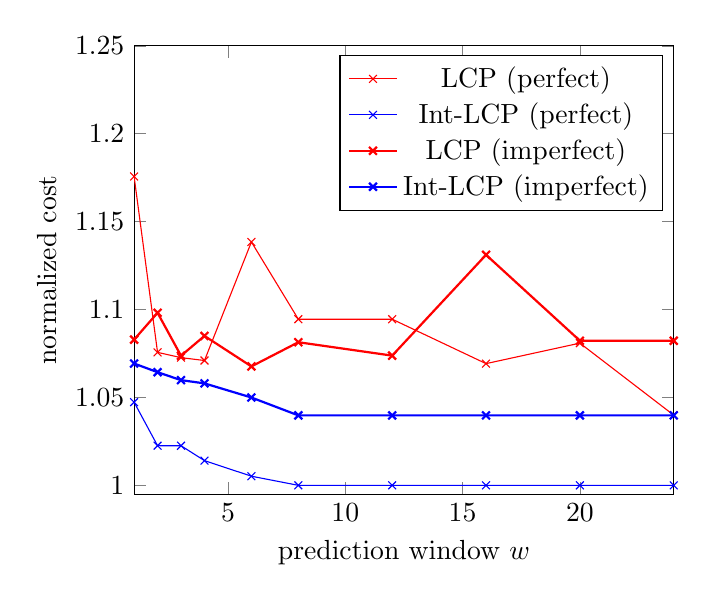
\begin{tikzpicture}

\begin{axis}[
% tick align=outside,
% tick pos=left,
% x grid style={white!69.0196078431373!black},
xlabel={prediction window $w$},
xmin=1, xmax=24,
% xtick style={color=black},
% y grid style={white!69.0196078431373!black},
ylabel={normalized cost},
ymin=0.995, ymax=1.25,
% ytick style={color=black}
]
\addplot [mark=x,red]
table {%
0 1.098736948
1 1.175687427
2 1.075631818
3 1.072634645
4 1.070999275
6 1.138422029
8 1.094499546
12 1.094499546
16 1.06923045
20 1.080885023
24 1.039921325
};
\addlegendentry{LCP (perfect)}
\addplot [mark=x,blue]
table {%
0 1.134416689
1 1.047299695
2 1.022549638
3 1.022528928
4 1.014063942
6 1.00519416
8 1
12 1
16 1
20 1
24 1
};
\addlegendentry{Int-LCP (perfect)}
\addplot [mark=x,red,thick]
table {%
0 1.098736948
1 1.082887541
2 1.098133413
3 1.073693844
4 1.08498568
6 1.067637295
8 1.081397557
12 1.073772973
16 1.13110595
20 1.08225852
24 1.08225852
};
\addlegendentry{LCP (imperfect)}
\addplot [mark=x,blue,thick]
table {%
0 1.134416689
1 1.069284948
2 1.064359748
3 1.059832012
4 1.057992166
6 1.049956689
8 1.039784723
12 1.039784723
16 1.039784723
20 1.039784723
24 1.039784723
};
\addlegendentry{Int-LCP (imperfect)}
\end{axis}

\end{tikzpicture}
}
    \caption{LCP and Int-LCP}\label{fig:case_studies:predictions:lcp}
    \end{subfigure}
    \begin{subfigure}[b]{.4825\linewidth}
    \resizebox{\textwidth}{!}{% This file was created by tikzplotlib v0.9.9.
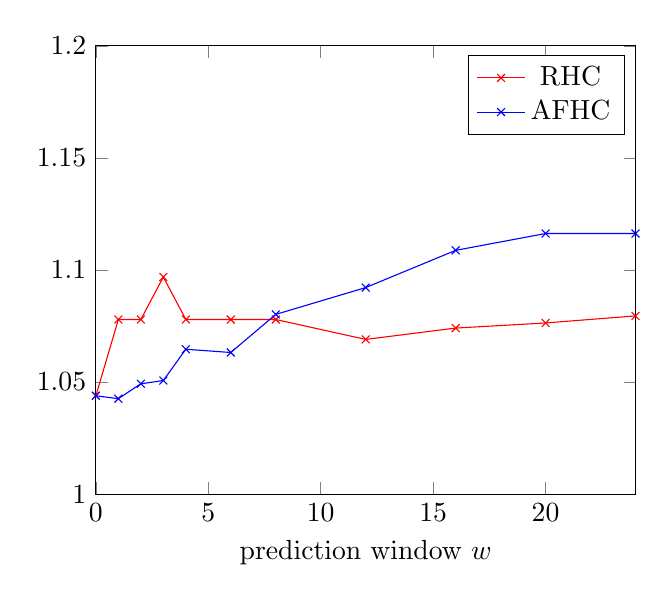
\begin{tikzpicture}

\begin{axis}[
% tick align=outside,
% tick pos=left,
% x grid style={white!69.0196078431373!black},
xlabel={prediction window $w$},
xmin=0, xmax=24,
% xtick style={color=black},
% y grid style={white!69.0196078431373!black},
% ylabel={normalized cost},
ymin=1, ymax=1.2,
% ytick style={color=black}
]
\addplot [mark=x,red]
table {%
0 1.043876404
1 1.077904071
2 1.077904071
3 1.096849433
4 1.077911928
6 1.077904071
8 1.077904071
12 1.06902603
16 1.0740756
20 1.076362197
24 1.079518259
};
\addlegendentry{RHC}
\addplot [mark=x,blue]
table {%
0 1.043876404
1 1.042590748
2 1.049217045
3 1.050676806
4 1.064636454
6 1.063182574
8 1.080176738
12 1.092145632
16 1.108752789
20 1.116262537
24 1.116262537
};
\addlegendentry{AFHC}
\end{axis}

\end{tikzpicture}
}
    \caption{RHC and AFHC}\label{fig:case_studies:predictions:mpc}
    \end{subfigure}
    \caption{Performance of online algorithms with a prediction window for the Alibaba trace. The left figure shows the performance of LCP and Int-LCP. The right figure shows the performance of RHC and AFHC. Note that LCP does not continuously approach the normalized cost $1$ as $w \to 24$ because of numerical inaccuracies solving the convex optimizations and as the obtained is compared to the integral offline optimum rather than the fractional offline optimum. For RHC and AFHC, the achieved normalized cost is independent of whether perfect predictions or the predictions from \cref{fig:case_studies:predictions:prediction} are used.}
\end{figure}
